% -*- mode: noweb; noweb-default-code-mode: R-mode; -*-
\documentclass[a4paper]{book}
%\documentclass[envcountsame,envcountchap]{svmono}


\usepackage{graphicx,url}
\usepackage{amssymb}

\def\pf{{\bf Proof. }}
\def\logimplies{\Rightarrow}
\def\convinlaw{\stackrel{{\cal L}}{\Longrightarrow }}
\def\convinp{\stackrel{P}{\longrightarrow }}
\def\convas{\stackrel{a.s.}{\longrightarrow }}
\def\convv{\stackrel{v}{\longrightarrow}}
\def\asymp{\stackrel{{\mathbb P}}{\sim}}
\def\RR{\mathbb R}
\def\ZZ{\mathbb Z}
\def\QQ{\mathbb Q}
\def\NN{\mathbb N}
\def\MM{\mathbb M}
\def\LL{\mathbb L}
\def\EE{\mathbb E}
\def\PP{\mathbb P}
\def\DD{\mathbb D}
\def\WW{\mathbb W}
\def\FF{\mathbb F}
\def\II{\mathbb I}
\def\FF{\mathbb F}
\def\XX{\mathbb X}
\def\CC{\mathbb C}
\def\sige{\sigma_{\epsilon}}
\def\ttheta{\widetilde{\theta}}
\def\tTheta{\widetilde{\Theta}}
\def\tsig{\widetilde{\sigma}^2}
\def\tc{\widetilde{c}}
\def\etheta{\widehat{\theta}}
\def\eTheta{\widehat{\Theta}}
\def\esig{\widehat{\sigma}^2}
\def\ptheta{\underline{\theta}}
\def\pTheta{\underline{\Theta}}
\def\psig{\underline{\sigma}^2}

\def\eqinlaw{\stackrel{{\cal L}}{=}}
\def\tends{\rightarrow}
\def\tendsinf{\rightarrow\infty}
\def\isodynamo{\Leftrightarrow}

\newtheorem{Theorem}{Theorem}
\newtheorem{Lemma}{Lemma}
\newtheorem{Corollary}{Corollary}
\newtheorem{Proposition}{Proposition}
\newtheorem{Definition}{Definition}
\newtheorem{Remark}{Remark}
\newtheorem{Example}{Example}
\newtheorem{Exercise}{Exercise}
\newtheorem{Illustration}{Illustration}
\newcommand{\mbf}[1]{\mbox{\boldmath $#1$}}

\setlength{\textwidth}{6.5in} \setlength{\textheight}{9in}
\setlength{\evensidemargin}{12pt} \setlength{\oddsidemargin}{0in}
\setlength{\topmargin}{1in}
\renewcommand{\baselinestretch}{1.3}
\setlength{\headheight}{0.2in} 
\setlength{\headsep}{0.2in}

%- Makes the section title start with Appendix in the appendix environment
\newcommand{\Appendix}
{%\appendix
%\def\thesection{Appendix~\Alph{section}}
\def\thesection{Appendix~\Alph{chapter}}
%\def\thesubsection{\Alph{section}.\arabic{subsection}}
%\def\thesubsection{A.\arabic{subsection}}
\def\thesubsection{A.\arabic{section}}
}


%\pagestyle{empty}
\usepackage{amssymb}
\usepackage{amsmath}
\usepackage{latexsym}
\usepackage{epsfig}
%\usepackage{html}
\usepackage{verbatim}
\usepackage{hyperref}
\usepackage{float}
\usepackage[utf8]{inputenc}
\usepackage{a4wide}

\title{Multivariate Real-Time Signal Extraction}
\author{Marc Wildi and Tucker McElroy}




\usepackage{Sweave}
\begin{document}

\maketitle

\date{}

%\SweaveOpts{prefix.string=c:/wia/tmp/bar}

\frontmatter%%%%%%%%%%%%%%%%%%%%%%%%%%%%%%%%%%%%%%%%%%%%%%%%%%%%%%

%\include{dedic}
%\newpage
%\phantom{rete}
%\newpage
%\include{preface}




\tableofcontents


\mainmatter%%%%%%%%%%%%%%%%%%%%%%%%%%%%%%%%%%%%%%%%%%%%%%%%%%%%%%%

%-----------------------------------------------

% Chapter 1
% Parallelized computation chapters customization and replication
% simanz<-100 chapters customization and replication
% Load all chapters

\chapter{Introduction}\label{intro_sec}

\section{Overview}

\subsection{Signals and Extraction}

In the applications of time series analysis to macroeconomics, finance, and quality control
 it is essential to extract useful information about trends, turning points, and anomalies
 in real time.  The practitioner does not have the luxury of sifting past data for 
 structural breaks, indicators of regime change, or changes to volatility.  Informative elections are
 contingent upon understanding the dynamics of various time series at time present.  Because
 long-term movements, as well as aberrations, are defined in terms of the long-run behavior of a 
 time series over past, present, and future, any analysis of the present state necessarily involves
 a degree of forecasting.  This  broad topic is referred to as real-time signal extraction.

A signal is any component of a time series that is deemed useful for a particular application.  
If long-term movements are of interest, the signal is a trend.  If short-term fluctuations about
 a longer-term mean are of interest, the signal is a cycle.  If shocks, due to rare
 terrorist events or natural disasters, are of interest, the signal consists of the extreme values.
 If regular patterns of an annual period, linked to cultural or meteorological patterns, are of interest,
 the signal is a seasonal component.

However, these signals are not directly observable at time present, because in each case their
 definition involves all the past and future values of a time series -- but the future is unknown,
 and only part of the past is available to us.  The statistical processes by which a signal is
 estimated from available data is referred to as extraction, and the residual from the 
 signal extraction is referred to as the noise.  Whereas signals can be estimated from historical, or past,
 sections of a time series, when effort is focused upon time present we refer to the analysis as
 real-time signal extraction.

Real-time signal extraction is considerably more challenging, and useful, than historical signal extraction.
 The difficulty lies in the uncertainty about the future, which is transmitted unto the signal 
 extraction estimates themselves.  One way to conceive of this difficulty is through the warring
 principles of timeliness and accuracy: should we procrastinate in providing our analysis of the present,
 we can increase the accuracy of signal extraction, but our answers become less relevant, even as the present
 time rapidly drifts into the past.  Conversely,   extremely timely extractions suffer from 
 greater future uncertainty, and are likely to exhibit inaccuracy.

There is a considerable body of literature addressing signal extraction, but this book focuses upon
 a particular methodology called Direct Filter Analysis (DFA).  As the original development of DFA
 was univariate, the methodology's power was limited to the information content
 within a single time series.  But because batches of time series can be closely linked, exhibiting 
 correlated trends, common dynamics, or even predictive relationships, it is natural to expect that
 a multivariate extension of DFA to vector time series will more greatly facilitate informed decision 
 making.  The topic of this book is Multivariate Direct Filter Analysis (MDFA).

 

\subsection{The Classic Model-Based Paradigm}

Many signals can be formulated as weighted linear combinations of a time series, in which case the real-time
 signal extraction problem can be approached as a Linear Prediction Problem (LPP).  In order to pose
 an LPP, a solution criterion is needed, and Mean Squared Error (MSE) is often used: one seeks a real-time 
 signal extraction that has minimal MSE discrepancy with the actual target signal.  Although an LPP
 can then be solved, the solution depends on knowing something about the dynamics in the time series process.
 The most venerable approach to understanding these dynamics is to posit a time series model, and fit
 this model to the observed data.  This approach, which goes back to the work of Yule in the 1930s, is called
 the classic paradigm, being based upon a Model-Based Analysis (MBA).

An attractive feature of MBA is that analytical formulas for the LPP solutions can often be obtained, thereby
 facilitating computation.  The philosophy underpinning the classic paradigm is that a Data Generation Process (DGP)
 exists -- as a theoretical, or Platonic construct -- to which the observed data closely adheres.  Formally,
 the DGP is some stochastic process defined upon a probability space, and the observed data is a realization, or sample path, of
 the DGP.  Statistical inference is involved with the science of identifying a model class for the DGP, narrowing down
 the class to a particular model (by eliminating contenders), and fitting that model via fixing values of the parameters.
 Successive applications of model diagnostics allow for refinements, and a process by which we can verify the validity
 of a postulated model.  Of course, all of this is done on the basis of the single realization of the DGP.

While recognizing that any such model need not be correct, i.e., exactly match the DGP itself, such models can yet
 be useful to the extent to which they reflect important features in the data.  Yet it is difficult to keep a model
 simple -- which is necessay to its utility -- and at the same time be sufficiently versatile to explain all the 
data's features.  Moreover, the appellation of importance is subjective: a feature deemed important to one user may
 be irrelevant to another.  This begs the question of customization: each user, with a distinct set of criteria and
 desired applications, could potentially stress the importance of a subset of features at the cost of de-emphasizing others.
 The classic paradigm ignores, or at least passes over, the issue of customization, and proposes a single all-purpose
 concept of utility: the minimization of one-step ahead forecast error MSE.

 Another term for this classic conception of model utility is the Wold decomposition, which breaks a wide class of
 stochastic processes down in terms of a component that is completely predictable from its own infinite past, and 
 a second component fully describable in terms of one-step ahead forecast errors.  Classical models can then
 be viewed as attempts to approximate the linear machinery in the Wold decomposition.    However, were attention to
 focus upon an alternative utility, e.g., 10-step ahead forecasting, a different class of models would be suggested,
 with different apparatus for model selection, fitting, and evaluation.

However, customizing the modeling apparatus to allow for specific applications offers only a partial solution, because
 model mis-specification is the larger challenge.  The full set of LPP solutions for a given time series is greatly
 constrained once a model is introduced, as only a particular subset of solutions can be obtained.  If the model is
 badly mis-specified, the resulting LPP solution will be inadequate, even if the criteria for model selection are customized.
 This empirical disfunctionality motivated the genesis of DFA, which essentially provides access to a much wider
 pool of LPP solutions.  Moreover, the basic DFA can be easily modified to allow for direct customization of 
real-time problems, according to whether users are concerned with timeliness, accuracy, or fidelity to the original signal (called
 smoothness).  
 

%Marc's perspective:
%\begin{itemize}
%\item Maximum Likelihood, main purpose: determine DGP. If DGP is known then optimality can be invoked, in principle. 
%\item Problem: model misspecification. Pseudo maximum likelihood: one-step ahead mean-square criterion. 
%\item Emphasizes short-term performances, only (contrast with real-time trend extraction: long-term component). 
%\item Rigid criterion: can account neither for relevant problem-structure (signal extraction=one and multi-step ahead forecasts) nor for various user-priorities (ATS-trilemma).
%\end{itemize}

\subsection{The Scope of MDFA}

Our critique of the classic paradigm has several facets.  First, there is typically model mis-specification present.  Second, the problem
 has typically not been structured properly, in the sense that the criteria used do not correspond to the relevant LPP, but rather to
   one-step ahead forecasting.  Third, there is no specific customization of the model, in order to account for timeliness and accuracy.
 These weaknesses are actually linked together.  

Model mis-specification is always present; the issue is whether it has a significant impact upon the objectives of analysis.  For instance,
 a given model's mis-specification may have grave repercussions for certain problem structures, while being adequate for other LPPs.
 The given LPP of interest determines the gravity and impact of model mis-specification.  Moreover, in the classic paradigm the one-step
 ahead forecasting LPP is solved, and it is merely hoped that timeliness and accuracy will be adequate for all users.  Model parameters
 can be tweaked, or tuned, in order to indirectly modify timeliness and accuracy -- but the relationships are indirect and often poorly
 understood.  By building the timeliness-accuracy tradeoff directly into the DFA criterion, the optimality of an LPP solution for a
 customized application is assured.

These topics have been treated in Wildi and McElroy (2016) in the case of univariate time series, which discusses at length
 the basic \href{http://blog.zhaw.ch/sef/files/2014/10/DFA.pdf}{DFA} (Sweave environment: replication).  This book presents
 the generalized treatment of the multivariate LPP in   Chapter \ref{mse_sec}. But before discussing customization in Chapter \ref{ats_sec},
 we discuss the applications of forecasting and nowcasting, as well as the impact of data vintage, in  Chapter \ref{fil_sec}).
 Then the basic LPP treatment is extended to nonstationary processes in Chapter \ref{int_sec}, followed by a discussion of filter constraints (Chapter \ref{con_sec}).
  This treatment is extended to the case of co-integration in Chapter \ref{coint_sec}.   Applications to replicating and enhancing classical model-based approaches and HP/CF-filters 
 are given in Chapter \ref{rep_sec}, while  more sophisticated gain/loss structures  are discussed in Chapter \ref{exo_sec}.
Additional topics include inference (Chapter \ref{inf_sec}), regularization (Chapter \ref{reg_sec}), data revisions (Chapter \ref{rev_sec}),
 mixed-frequency data (Chapter \ref{mix_sec}), and   adaptive filtering (Chapter \ref{ada_sec}).

\section{The Style of the Book}

This book was generated using Sweave, in accordance with the philosophy of 
 scientific replicability.  Throughout the text are portions of R code that
 can be pasted into an R script and directly run, given that the user
 has certain packages already installed.  This installation is described below.
 
\subsection{Setting the Paths}

Begin by clearing the workspace: 
\begin{Schunk}
\begin{Sinput}
> #rm(list=ls())
\end{Sinput}
\end{Schunk}
The R code in   various chapters of this book requires installation of the following R packages:
\begin{Schunk}
\begin{Sinput}
> # Load packages: time series and xts
> #library(tseries)
> library(xts)
> # State-space models (will be replicated by MDFA) 
> library(dlm)
> # Classic filter designs (be replicated by MDFA)
> library(mFilter)
> # Numerical package 
> library(numDeriv)
> # Graphical package for recession-shading (empirical examples based on US-GDP)
> library(tis)
> # Library for tables
> library(Hmisc)
> require(xtable)
> #install.packages("devtools")
> library(devtools)
> # Load MDFA package from github
> devtools::install_github("wiaidp/MDFA")
> # MDFA package
> library(MDFA)
\end{Sinput}
\end{Schunk}
US-GDP data for the empirical examples can be retrieved either directly from 
 Quandl (requiring a preliminary user registration) or from a local data folder,
  which is the default-setting:
\begin{Schunk}
\begin{Sinput}
> # Load fresh data from quandl: T/F
> #   Default-setting is False: the data will be loaded from local data folder
> load_from_quandl <- F
\end{Sinput}
\end{Schunk}
Paths to MDFA code, as well as to the US-GDP data, must be provided. 
 It is assumed that the MDFA package is saved to a main folder containing
 subfolders labeled as DFA, MDFA, model-based, and data. 
The R code in the book generates pdf graphs that are saved in a separate folder, 
whose path is specified by {\em path.out}.
\begin{Schunk}
\begin{Sinput}
> # Set main path
> path.main <- paste(getwd(),"/Sweave/",sep="")
> #path.main <- "C:\\Users\\Tucker\\Documents\\MDFAbook\\"
> # Set paths to subfolders
>   # Path to Latex-folder: all pdfs generated by the R code are filed there
> path.out <- paste(path.main,"Latex/",sep="")
>   # Path to data (US-GDP)
> path.dat <- paste(path.main,"Data/",sep="")
>   # Path to code that is part of MDFA-Legacy project but not part of MDFA package 
> path.pgm <- paste(path.main,"R/",sep="")
\end{Sinput}
\end{Schunk}
The univariate DFA code is the same as in \href{http://blog.zhaw.ch/sef/files/2014/10/DFA.pdf}{DFA}; all 
 empirical examples are and will be fully compatible. 

\subsection{DFA}\label{dfa_intro}
We here briefly review the relevant facets of \href{http://blog.zhaw.ch/sef/files/2014/10/DFA.pdf}{DFA},
 thereby providing an anchor for the MDFA discussion. 

\subsubsection{DFT and Periodogram}

The Discrete Fourier Transform (DFT) and the periodogram are defined in Sections 2.2 and 2.3 of
\href{http://blog.zhaw.ch/sef/files/2014/10/DFA.pdf}{DFA}.  
The following periodogram function -- referred to as {\em per} below --
  in the MDFA package replicates these formulae.  Note that frequency $\pi$ is treated differently, depending on
 whether the  sample size is odd or even; also, the value at frequency zero is scaled by $1/\sqrt{2}$,
  which  is explained in later text.  
\begin{Schunk}
\begin{Sinput}
> head(per,100)
\end{Sinput}
\begin{Soutput}
1  function (x, plot_T)                                                              
2  {                                                                                 
3      len <- length(x)                                                              
4      per <- 0:(len/2)                                                              
5      DFT <- per                                                                    
6      for (k in 0:(len/2)) {                                                        
7          cexp <- exp((0+1i) * (1:len) * 2 * pi * k/len)                            
8          DFT[k + 1] <- sum(cexp * x * sqrt(1/(2 * pi * len)))                      
9      }                                                                             
10     if (abs(as.integer(len/2) - len/2) < 0.1)                                     
11         DFT[k + 1] <- DFT[k + 1]/sqrt(2)                                          
12     per <- abs(DFT)^2                                                             
13     if (plot_T) {                                                                 
14         par(mfrow = c(2, 1))                                                      
15         plot(per, type = "l", axes = F, xlab = "Frequency", ylab = "Periodogram", 
16             main = "Periodogram")                                                 
17         axis(1, at = 1 + 0:6 * len/12, labels = c("0", "pi/6",                    
18             "2pi/6", "3pi/6", "4pi/6", "5pi/6", "pi"))                            
19         axis(2)                                                                   
20         box()                                                                     
21         plot(log(per), type = "l", axes = F, xlab = "Frequency",                  
22             ylab = "Log-periodogram", main = "Log-periodogram")                   
23         axis(1, at = 1 + 0:6 * len/12, labels = c("0", "pi/6",                    
24             "2pi/6", "3pi/6", "4pi/6", "5pi/6", "pi"))                            
25         axis(2)                                                                   
26         box()                                                                     
27     }                                                                             
28     return(list(DFT = DFT, per = per))                                            
29 }                                                                                 
\end{Soutput}
\end{Schunk}
This function will be generalized in the new multivariate setting.

\subsubsection{Basic DFA}

A simple   version of the DFA  based on the MSE criterion alone -- 
 as proposed in Section 4.1 of \href{http://blog.zhaw.ch/sef/files/2014/10/DFA.pdf}{DFA} --
 is included in the MDFA package:  

\begin{Schunk}
\begin{Sinput}
> # This function computes MSE DFA solutions 
> # L is the length of the MA filter,
> # periodogram is the frequency weighting function in the DFA
> # Gamma is the transfer function of the symmetric filter (target) and
> # Lag is the lag-parameter: Lag=0 implies real-time filtering, Lag=L/2
> #     implies symmetric filter
> # The function returns optimal coefficients as well as the transfer 
> #     function of the optimized real-time filter
> head(dfa_ms,100)
\end{Sinput}
\begin{Soutput}
1  function (L, periodogram, Lag, Gamma)                                    
2  {                                                                        
3      periodogram[1] <- periodogram[1]/2                                   
4      K <- length(periodogram) - 1                                         
5      X <- exp(-(0+1i) * Lag * pi * (0:(K))/(K)) * rep(1, K + 1) *         
6          sqrt(periodogram)                                                
7      X_y <- exp(-(0+1i) * Lag * pi * (0:(K))/(K)) * rep(1, K +            
8          1)                                                               
9      for (l in 2:L) {                                                     
10         X <- cbind(X, (cos((l - 1 - Lag) * pi * (0:(K))/(K)) +           
11             (0+1i) * sin((l - 1 - Lag) * pi * (0:(K))/(K))) *            
12             sqrt(periodogram))                                           
13         X_y <- cbind(X_y, (cos((l - 1 - Lag) * pi * (0:(K))/(K)) +       
14             (0+1i) * sin((l - 1 - Lag) * pi * (0:(K))/(K))))             
15     }                                                                    
16     xtx <- t(Re(X)) %*% Re(X) + t(Im(X)) %*% Im(X)                       
17     b <- as.vector(solve(xtx) %*% (t(Re(X_y)) %*% (Gamma * periodogram)))
18     trffkt <- 1:(K + 1)                                                  
19     trffkt[1] <- sum(b)                                                  
20     for (k in 1:(K)) {                                                   
21         trffkt[k + 1] <- (b %*% exp((0+1i) * k * (0:(length(b) -         
22             1)) * pi/(K)))                                               
23     }                                                                    
24     return(list(b = b, trffkt = trffkt))                                 
25 }                                                                        
\end{Soutput}
\end{Schunk}
This function is nested in the multivariate MDFA,
  in the sense that the latter can replicate the former perfectly when suitably parametrized;
 see Section \ref{ex_rep_dfa} below.



\subsubsection{Customized DFA}

A more general DFA function, called \emph{dfa\textunderscore analytic}, is proposed in Section 4.3.5 of
\href{http://blog.zhaw.ch/sef/files/2014/10/DFA.pdf}{DFA}. Customization and the generic 
 Accuracy-Timeliness-Smoothness (ATS) trilemma are presented in Sections 4.3 and 5 of
 \href{http://blog.zhaw.ch/sef/files/2014/10/DFA.pdf}{DFA}. This function is included in the MDFA package: 
\begin{Schunk}
\begin{Sinput}
> head(dfa_analytic)
\end{Sinput}
\begin{Soutput}
1 function (L, lambda, periodogram, Lag, Gamma, eta, cutoff, i1, 
2     i2)                                                        
3 {                                                              
4     periodogram[1] <- periodogram[1]/2                         
5     lambda <- abs(lambda)                                      
6     eta <- abs(eta)                                            
\end{Soutput}
\end{Schunk}
The additional control parameters {\em lambda}, {\em eta} allow for customization of the filter,  as discussed below
 in Chapter \ref{ats_sec}.  The Boolean {\em i1} and {\em i2}
  can enforce useful filter constraints; see Chapter \ref{con_sec}. This function is also encompassed by the   MDFA. 



\subsection{MDFA}\label{mdfa_intro}

The R code for MDFA is more sophisticated than that of the DFA, and is correspondingly more complex and lengthy. 
 As for the DFA package, the MDFA code can be sourced. We here briefly review the corresponding pieces.


\subsubsection{Data Matrix}

All time series are collected in a data-\emph{matrix}, say $X$, which is organized as follows: 
\begin{itemize}
\item the first column $X[,1]$ of $X$ always corresponds to the target series: the target series $X[,1]$ is the time series
 to be forecasted, nowcasted or backcasted.
\item Columns $2$, $3$, $\ldots$ of $X$ are allocated to the explanatory variables (more than one in a multivariate setting). 
If the target series is part of the set of explanatory variables (it does not have to be), then it must be assigned a specific column 
-- by convention always the second one -- in $X$, i.e., in this case the target series is entered twice, in the first column (target) and
  in the second column (explanatory data).     
\end{itemize}

\noindent {\bf Example}.  Suppose we study a  two-dimensional signal extraction problem, whereby the target series (first column) 
is part of the set of explanatory variables:
\begin{Schunk}
\begin{Sinput}
> set.seed(1)
> len <- 100
> target <- arima.sim(list(ar=0.9),n=len)
> explanatory_2 <- target+rnorm(len)
> explanatory <- cbind(target,explanatory_2)
> x <- cbind(target,explanatory)
> dimnames(x)[[2]] <- c("target","explanatory 1","explanatory 2")
> head(x)
\end{Sinput}
\begin{Soutput}
       target explanatory 1 explanatory 2
[1,] 1.703613      1.703613     0.3191863
[2,] 1.398197      1.398197     3.2674879
[3,] 3.659995      3.659995     4.0850957
[4,] 3.254756      3.254756     3.0161086
[5,] 3.619020      3.619020     4.6775026
[6,] 3.285120      3.285120     4.1715424
\end{Soutput}
\end{Schunk}
For a one-step ahead forecast LPP, we might consider lagging both the explanatory variables:
\begin{Schunk}
\begin{Sinput}
> x<-cbind(x[,1],lag(x[,2:3],-1))
> dimnames(x)[[2]]<-c("target","lagged explanatory 1","lagged explanatory 2")
> head(x)
\end{Sinput}
\begin{Soutput}
       target lagged explanatory 1 lagged explanatory 2
[1,] 1.703613                   NA                   NA
[2,] 1.398197             1.703613            0.3191863
[3,] 3.659995             1.398197            3.2674879
[4,] 3.254756             3.659995            4.0850957
[5,] 3.619020             3.254756            3.0161086
[6,] 3.285120             3.619020            4.6775026
\end{Soutput}
\end{Schunk}
 By adopting the frequency-domain methods of this book, we can generalize this construction and
    avoid the introduction of missing values (denoted by NA in R).  $\quad \Box$


\subsubsection{DFT}

In contrast to the univariate DFA, where the LPP can be expressed in terms of  the periodogram, the multivariate case 
 requires the   DFT of each time series in order to account for cross-sectional dependencies.  These DFTs are complex-valued
 quantities, and the angular portion of the cross-spectrum provides information about the relative phase-shift of each explanatory time series. 
  In the univariate case the relative phase-shift is irrelevant, because the target series and the explanatory series are identical.
 The scope of the method is extended in order to cover the mixed-frequency case, which is discussed in Chapter \ref{mix_sec}. 
 Another facet, is that we allow for the possibility of integrated processes; see Chapter \ref{int_sec}. 
 In order to illustrate some of the new features we briefly look at the main DFT function called {\em spec\textunderscore comp}:
\begin{Schunk}
\begin{Sinput}
> spec_comp
\end{Sinput}
\begin{Soutput}
function (insamp, x, d) 
{
    if (d == 1) {
        weight_func <- periodogram_bp(diff(x[1:insamp, 1]), 1, 
            insamp - 1)$fourtrans
        if (length(weight_func) > 1) {
            for (j in 2:ncol(x)) {
                per <- periodogram_bp(diff(x[1:insamp, j]), 1, 
                  insamp - 1)$fourtrans
                weight_func <- cbind(weight_func, per)
            }
        }
    }
    else {
        weight_func <- periodogram_bp(x[1:insamp, 1], 0, insamp)$fourtrans
        if (length(weight_func) > 1) {
            for (j in 2:ncol(x)) {
                per <- periodogram_bp(x[1:insamp, j], 0, insamp)$fourtrans
                weight_func <- cbind(weight_func, per)
            }
        }
    }
    colnames(weight_func) <- colnames(x)
    return(list(weight_func = weight_func))
}
<bytecode: 0x000001ea32507de8>
<environment: namespace:MDFA>
\end{Soutput}
\end{Schunk}
The inner loop   tracks the columns of the data matrix $X$ and the DFTs are stored in a matrix called \emph{weight\textunderscore func},
  which is returned by the function. The matrix \emph{weight\textunderscore func} collects all DFTs;
  the target series is always in the first column, whereas the DFTs of the explanatory series are in columns $2$, $3$, $\ldots$
 The function \emph{periodogram\textunderscore bp}, called in the above loop, is slightly more general than the DFA 
function \emph{per} proposed in the previous section. In particular, it can handle various integration orders as well as
 seasonal peculiarities. 

\subsection{Using MDFA}\label{control_dfa}

\subsubsection{A Versatile User Interface}

MDFA is a generic forecast and signal extraction paradigm. Besides its capacity to  replicate classical time series approaches, 
  MDFA possesses unique features such as customization and regularization (Chapter \ref{reg_sec}); it can
  treat data revisions (Chapter \ref{rev_sec}), mixed-frequency problems (Chapter \ref{mix_sec}),
 and non-stationarity (Chapters \ref{int_sec} and \ref{coint_sec}. Accordingly, the user interface 
is more sophisticated than the precediing DFA package.
Consider the head of the main estimation routine:    

\begin{Schunk}
\begin{Sinput}
> head(mdfa_analytic)
\end{Sinput}
\begin{Soutput}
1 function (L, lambda, weight_func, Lag, Gamma, eta, cutoff, i1,             
2     i2, weight_constraint, lambda_cross, lambda_decay, lambda_smooth,      
3     lin_eta, shift_constraint, grand_mean, b0_H0, c_eta, weight_structure, 
4     white_noise, synchronicity, lag_mat, troikaner)                        
5 {                                                                          
6     lambda <- abs(lambda)                                                  
\end{Soutput}
\end{Schunk}
 Arguments such as  \emph{weight\textunderscore func} (discussed above), the filter length ($L$), and the target specification \emph{Gamma}
 are straightforward.    But there are numerous additional control parameters: the relevance and the modus operandi of these
 will be discussed in this book. 


\subsubsection{Default Settings}

For convenience, we store a so-called default setting of the parameters in a file called \emph{control\textunderscore default}.
 First we define the data (initialize the DFT matrix) and specify the filter  length:
\begin{Schunk}
\begin{Sinput}
> weight_func <- matrix(rep(1:6,2),ncol=2)
> L <- 2
\end{Sinput}
\end{Schunk}
Given these two entries (DFT and filter length), the default-settings are as follows:
\begin{Schunk}
\begin{Sinput}
> d<-0
> lin_eta<-F
> lambda<-0
> Lag<-0
> eta<-0
> i1<-F
> i2<-F
> weight_constraint<-rep(1/(ncol(weight_func)-1),ncol(weight_func)-1)
> lambda_cross<-lambda_smooth<-0
> lambda_decay<-c(0,0)
> lin_expweight<-F
> shift_constraint<-rep(0,ncol(weight_func)-1)
> grand_mean<-F
> b0_H0<-NULL
> c_eta<-F
> weights_only<-F
> weight_structure<-c(0,0)
> white_noise<-F
> synchronicity<-F
> cutoff<-pi
> lag_mat<-matrix(rep(0:(L-1),ncol(weight_func)),nrow=L)
> troikaner<-F
\end{Sinput}
\end{Schunk}
This particular configuration will be used extensively in Chapter \ref{mse_sec}; it corresponds to the basic MSE criterion 
 (i.e., no customization) without regularization, without design constraints, and without any {\em a priori} knowledge.
  Also, this configuration presumes a   common identical sampling frequency (i.e., no mixed frequency data)
 and the absence of data revisions. The default settings can be obtained by sourcing the corresponding R file:

\begin{Schunk}
\begin{Sinput}
> source(file=paste(path.pgm,"control_default.r",sep=""))
\end{Sinput}
\end{Schunk}
For later use we   source a convenient plotting function:
\begin{Schunk}
\begin{Sinput}
> source(file=paste(path.pgm,"mplot_func.r",sep=""))
\end{Sinput}
\end{Schunk}

\subsubsection{Selected Calls: Classic MSE, Customization and Regularization}

Selected calls of the classic MSE  criterion -- as well as calls utilizing the customization or regularization features --
 are available through dedicated functions in the MDFA package: 
\begin{Schunk}
\begin{Sinput}
> head(MDFA_mse)
\end{Sinput}
\begin{Soutput}
1 function (L, weight_func, Lag, Gamma) 
2 {                                     
3     cutoff <- pi                      
4     lin_eta <- F                      
5     lambda <- 0                       
6     eta <- 0                          
\end{Soutput}
\begin{Sinput}
> head(MDFA_mse_constraint)
\end{Sinput}
\begin{Soutput}
1 function (L, weight_func, Lag, Gamma, i1, i2, weight_constraint, 
2     shift_constraint)                                            
3 {                                                                
4     cutoff <- pi                                                 
5     lin_eta <- F                                                 
6     lambda <- 0                                                  
\end{Soutput}
\begin{Sinput}
> head(MDFA_cust)
\end{Sinput}
\begin{Soutput}
1 function (L, weight_func, Lag, Gamma, cutoff, lambda, eta)                  
2 {                                                                           
3     lin_eta <- F                                                            
4     weight_constraint <- rep(1/(ncol(weight_func) - 1), ncol(weight_func) - 
5         1)                                                                  
6     lambda_cross <- lambda_smooth <- 0                                      
\end{Soutput}
\begin{Sinput}
> head(MDFA_cust_constraint)
\end{Sinput}
\begin{Soutput}
1 function (L, weight_func, Lag, Gamma, cutoff, lambda, eta, i1, 
2     i2, weight_constraint, shift_constraint)                   
3 {                                                              
4     lin_eta <- F                                               
5     lambda_cross <- lambda_smooth <- 0                         
6     lambda_decay <- c(0, 0)                                    
\end{Soutput}
\begin{Sinput}
> head(MDFA_reg)
\end{Sinput}
\begin{Soutput}
1 function (L, weight_func, Lag, Gamma, cutoff, lambda, eta, lambda_cross,    
2     lambda_decay, lambda_smooth, troikaner = F, b0_H0 = NULL)               
3 {                                                                           
4     lin_eta <- F                                                            
5     weight_constraint <- rep(1/(ncol(weight_func) - 1), ncol(weight_func) - 
6         1)                                                                  
\end{Soutput}
\begin{Sinput}
> head(MDFA_reg_constraint)
\end{Sinput}
\begin{Soutput}
1 function (L, weight_func, Lag, Gamma, cutoff, lambda, eta, lambda_cross,      
2     lambda_decay, lambda_smooth, i1, i2, weight_constraint, shift_constraint, 
3     troikaner = F, b0_H0 = NULL)                                              
4 {                                                                             
5     lin_eta <- F                                                              
6     lin_expweight <- F                                                        
\end{Soutput}
\end{Schunk}
The heads of the corresponding functions differ in the number of additional arguments available 
when going from specific (MSE) to generic (reg).  The following chapters of the book provide an understanding of
 the use of these functions.



%----------------------------------------

% Chapter 2


\chapter{Linear Prediction Problems}
\label{chap:lpp}

\section{Background on Stationary Vector Time Series}

The reader should have a basic familiarity with multivariate time
 series analysis, such as that provided by L\"utkepohl (2007).  
 Our focus is on discrete-time stochastic processes taking values in $\RR^n$,
 and such will be denoted $\{ X_t \}$, i.e., a vector time series.
   Each $X_t$ for  a particular   $t \in \ZZ$ is a random vector 
 with $n$ components, and 
 the $j$th component will be denoted $X_{t,j}$ for $1 \leq j \leq n$.
  This can also be written as $X_{t,j} = e_j^{\prime} \, X_t$, where
 $e_j$ is the $j$th unit vector in $\RR^n$.  The union of these
 unit vectors is the $n \times n$ identity matrix, denoted $1_n$.

 In this book we are focused upon square integrable random variables,
 so that the classic Hilbert space projection theory (see, for example,
 Brockwell and Davis (1991)) can be applied.   Occasionally, we consider 
  vector time series $\{ Y_t \}$ or $\{ Z_t \}$, in which case the 
 same conventions apply.When $\{ X_t \}$ is 
 weakly stationary, its autocovariance function (acf)
 is defined for $h \in \ZZ$  via 
\[
   \Gamma (h) = \mbox{Cov} [ X_{t+h}, X_t ],
\]
 which does not depend upon $t$ by the stationarity assumption.  Recall
 that $\Gamma (-h) = { \Gamma (h) }^{\prime}$, and clearly
\[
   \Gamma_{jk} (h) = \mbox{Cov} [ X_{t+h,j}, X_{t,k} ]
\]
 for $1 \leq j,k \leq n$. The spectral density is a complex matrix-valued
 function of $\omega \in [-\pi, \pi]$, defined as the 
 Fourier Transform (FT) of the acf:
\[
   F (\omega) = \sum_{h \in \ZZ} \Gamma (h) \, z^h,
\]
 where we use the shorthand $z = e^{-i \omega}$.  Clearly,
\[
    F(-\omega) = 
   \sum_{h \in \ZZ} \Gamma (h) \, z^{-h} 
   = \sum_{h \in \ZZ} \Gamma (-h) \, z^h = 
  \sum_{h \in \ZZ} { \Gamma (h) }^{\prime} \, z^h = { F (\omega) }^{\prime},
\]
 which shows that the spectral density function (sdf) is Hermitian.
  In addition, its eigenvalues (for each $\omega$) are real and non-negative.
  Given a bounded sdf (i.e., each $F_{jk} $ has bounded modulus as a function
 of $\omega$), the acf can be recovered via inverse FT:
\begin{equation}
 \label{eq:spec2acf}
  \Gamma (h) = { \langle F  \rangle }_h
  =  \frac{1}{2 \pi} \int_{-\pi}^{\pi} F(\omega) \, e^{i \omega h}
  \, d\omega,
\end{equation}
 which uses the bracket notation to define the average integral of a 
 function (of $\omega$) multiplied by $e^{i \omega h} = z^{-h}$.

 The lag operator on a time series is denoted $L$, and is defined via
 the action
\[
  L X_t = X_{t-1}.
\]
  Powers  of $L$ are defined analogously, with $L^0 = 1$ (an operator
 identity) and negative powers yielding forward time shifts, i.e., leads.
 Matrix polynomials of $L$ yield new operators that act upon a time series
 using the linearity principal.  Thus, if $A(L) = \sum_{j=0}^a A_j \, L^j$
 for $n \times n$ matrices $A_j$, then
\[
  A(L) \, X_t = \sum_{j=0}^a A_j \, X_{t-j}.
\] 
  For many applications in this book, the polynomials are actually scalar,
 and can be interpreted as having coefficients $A_j$ given by an  
 identity matrix $1_n$ multiplied by a scalar coefficient $a_j$.
 
 The spectral representation of a stationary square integrable vector 
time series is particularly useful.  Assuming that $\EE X_t = 0$ (the
 zero vector in $\RR^n$) so that no fixed effects are present, we describe
 the stochastic process via
\begin{equation}
\label{eq:specRep}
  X_t = \int_{-\pi}^{\pi} e^{i \omega t} \, \mathcal{Z} (d\omega),
\end{equation}
 which is a stochastic integral computed with a Stieltjes measure
 $\mathcal{Z} (d\omega)$.  This is an orthogonal increments process,
 which mean $\mathcal{Z}$ is a random measure defined on ${[-\pi,\pi]}^n$
 that maps disjoint sets to independent random variables.  The actual
 distribution of the random measure is not our concern, but the particular
 orthogonal increments process associated with $\{ X_t \}$ has the 
 property that
\[
  \mbox{Cov} [ \mathcal{Z} (d\omega), \mathcal{Z} (d\xi) ]
   = {(2 \pi)}^{-1} \, F (\omega) \, d\omega \, 1_{ \{   \omega = \xi \} }
\]
 where $1_A$ is the indicator for the set $A$.
  (Also recall that for complex variables, a 
covariance involves conjugation of
 the second argument.)  This validates the expression
\[
  \mbox{Cov} [ X_{t+h}, X_t ] =
 \int_{-\pi}^{\pi}  \int_{-\pi}^{\pi} e^{i \omega (t+h)} \,
  e^{-i \xi t } \, \mbox{Cov} [ \mathcal{Z} (d\omega), 
  \mathcal{Z} (d\xi) ] 
 =  \frac{1}{2 \pi} \int_{-\pi}^{\pi} F(\omega) \, e^{i \omega h}
  \, d\omega = \Gamma (h).
\]
 As an example -- that furnishes a basic building block for subsequent processes --
 we have {\em white noise}, which refers to a mean zero $\{ X_t \}$ where 
 $F$ is constant, i.e.,
 $F(\omega) = \Sigma$ for all $\omega$, where $\Sigma $ is real and symmetric and
 non-negative definite.  Clearly, $\Gamma (h) = 0$ for $h \neq 0$ and $\Gamma (0) = \Sigma$.
 We denote this type of process with the notation $\mbox{WN} (\Sigma)$.

 The advantage of the spectral representation is that it quickly facillitates
 the understanding of linear filtering in the frequency domain.
 A multivariate filter maps one vector time series to another, and for
 now we suppose that both input and output belong to $\RR^n$.
 Linear filters can be expressed as matrix Laurent series in $L$:
\[
 \Psi (L) = \sum_{\ell \in \ZZ} \psi (\ell) \, L^{\ell},
\]
 where each $\psi (\ell)$ is an $n \times n$ matrix.  
 Individual entries of the matrix are denoted $\psi_{jk} (\ell)$,
 for $1 \leq j, k \leq n$.   We also use the notation
  $ {[\Psi (L) ]}^{s}_r $ to denote $\sum_{\ell=r}^s
  \psi (\ell) \, L^{\ell}$. 
     Another quantity of interest is the derivative of a filter, 
  defined via $\partial \Psi (L) = \sum_{j \in \ZZ} j \, \psi(j) \, L^{j-1}$.

  
  In the special case that $\Psi (L)$ is a power
 series in $L$, the only nonzero coefficients are for $\ell \geq 0$, 
 so that no negative powers of $L$ are featured, i.e., the filter
 only utilizes present and past data.  Such a filter is called a 
 {\em concurrent} filter.  
  The action of   a linear  filter
 on a weakly stationary time series,
 expressed in terms of the spectral representation, is
\[
  Y_t = \Psi (L) \, X_t = \sum_{\ell \in \ZZ} \psi (\ell) \, X_{t-\ell}
   = \sum_{\ell \in \ZZ} \psi (\ell)
  \, \int_{-\pi}^{\pi} e^{i \omega (t-\ell)} \,
   \mathcal{Z} (d\omega) =
  \int_{-\pi}^{\pi} e^{i \omega t} \, \Psi (e^{-i \omega}) \,
   \mathcal{Z} (d\omega).
\]
 So the output time series $\{ Y_t \}$ has orthogonal increments process
  $\Psi (z) \, \mathcal{Z} (d\omega)$, and in particular its sdf is
\[  
   \Psi (z) \, F(\omega) \, { \Psi (z) }^{*},
\]
 where $*$ denotes the conjugate transpose.  Thus, it is very natural
 to analyze a filter in terms of the function $\Psi (e^{-i \omega})$,
 which is called the {\em frequency response function} (frf).  In 
 the scalar case, an frf can be further dissected via the polar 
 decomposition of a complex number, yielding its {\em gain function}
 (the modulus) and the {\em phase function} (its angular portion).  
  Note that the coefficients are recovered from the frf via the inverse FT:
\[
  \psi (\ell) = {\langle \Psi (e^{-i \cdot } ) \rangle }_{\ell}.
\]
  It is well-known from Fourier theory that the degree of smoothness of a
 function at $\omega = 0$ corresponds to the degree of decay in the coefficients 
 of its  inverse FT.  In particular, when the frf is smooth and flat in a
 neighborhood of the origin then the matrix norm of the 
 coefficients $\psi (\ell)$ decays rapidly as $|\ell| \tends \infty$.  Conversely,
 discontinuities in the frf indicates slowly decaying coefficients.

 Datasets are typically available as a finite set of contiguous regular
 measurements, denoted $\{ x_1, x_2, \ldots, x_T \}$, where $T$ is 
 the length of sample.  The data is viewed as a realization of the 
 corresponding random vectors $\{ X_1, X_2, \ldots, X_T \}$, or alternatively
 as a time window of the sample path $\{ x_t \}$ corresponding to times
 $1, 2, \ldots, T$.  Applying the {\em vec} operator to such a sample
 yields the full vector $\underline{X}$, which is given by
\[
 \underline{X} = \mbox{vec} [ X_1, X_2, \ldots, X_T ].
\]
 The covariance matrix of this $nT$-dimensional random vector, in the
 stationary case, is block Toeplitz,   Each block is $n \times n$, and
 the $st$th such block, for $1 \leq s,t \leq T$, is given by $\Gamma (s-t)$.
 Also, from the sample we can compute the {\em Discrete Fourier Transform} (DFT)
  via
\begin{equation}
\label{eq:dft-def}
    \widetilde{X} (\omega) = T^{-1/2} \, \sum_{t=1}^T z^t \, X_t.
\end{equation}
 This can be computed for any $\omega \in [-\pi, \pi]$, though if we restrict
 to Fourier frequencies -- of the form
 $2 \pi j/T$ for integer $j$ -- then the various real and imaginary 
components of the DFT will be asymptotically uncorrelated, and
 also asymptotically normal.   The multivariate {\em periodogram}
  is defined to   be the rank one Hermitian matrix
\begin{equation}
\label{eq:per-def}
  \widehat{F} (\omega) = \widetilde{X} (\omega) \, { \widetilde{X} (\omega) }^*.
\end{equation}
  The periodogram furnishes a basic estimate of the spectral density $F$ of the process.
  There is an empirical version of (\ref{eq:spec2acf}), where the periodogram is mapped to the sample 
 autocovariance:
\begin{equation}
 \label{eq:per2acf}
  \widehat{\Gamma} (h) = { \langle \widehat{F}  \rangle }_h
  =  \frac{1}{2 \pi} \int_{-\pi}^{\pi} \widehat{F}(\omega) \, e^{i \omega h}
  \, d\omega.
\end{equation}
   This is easily verified using the definition of sample autocovariance
\[
   \widehat{\Gamma} (h) = T^{-1} \, \sum_{t=1}^{T-h}
   X_{t+h} \, X_t^{\prime}
\]
 for $h \geq 0$, and with $\widehat{\Gamma} (h) = { \widehat{\Gamma} (-h) }^{\prime}$ for $h < 0$.
  Conversely, the periodogram is the FT of the sample autocovariances:
\begin{equation}
 \label{eq:acf2per}
   \widehat{F} (\omega) = \sum_{|h| < T} \widehat{\Gamma} (h) \, e^{-i   \omega h}.
\end{equation}

\section{MSE Optimal Prediction Problems}

\subsection{The Linear Prediction Problem} We define the class of
real-time estimation problems considered in this book.  This chapter
 focuses upon the case of weakly stationary vector time series, but
 Chapter \ref{chap:int} makes extensions to difference stationary processes.

\begin{Definition} \rm
\label{def:target}
 A {\bf target} is defined to be the output of any known linear
 filter acting on the data process, i.e.,  $\{Y_t \}$ is a target
 time series corresponding to a given filter $\Psi (L)$ acting on a 
given observed time series
 $\{ X_t \}$ if and only if we can write for all integers $t$
\[
 Y_t = \Psi (L) X_t.
\] 
 We say that $\{ Y_t \}$ is a {\bf scalar target} if $\Psi (L)$ is a
 $1 \times n$-dimensional filter.
\end{Definition}

We are only interested in scalar targets.  The reason is that if $\{ Y_t \}$
 is multivariate, we can treat each component series $\{ Y_{t,j} \}$ for
 $1 \leq j \leq n$ in turn, so that without loss of generality we
 can just give the treatment for the scalar case. 

\begin{Example} {\bf  Multi-step Ahead Forecasting.}   \rm
\label{exam:multi-step.fore}
  Suppose that our goal is to forecast one of the component series 
 $h$ steps ahead, where $h \geq 1$ is the given {\em forecast lead}.
  Here, suppose that the series of interest is the first component, so 
 that 
\[
  Y_t = X_{t+h,1}
\]
  for all $ t \in \ZZ$.  This is indeed a scalar target, setting
  $\Psi (L) = L^{-h} \, e_1^{\prime}$.  That is, each $\psi (\ell)$
 is a $1 \times n$ row vector, each of which are zero except $\psi (-h)$,
 which is given by $e_1^{\prime}$.
\end{Example}

\begin{Example} {\bf Ideal Low-Pass.} \rm
\label{exam:ideal-low}
 In order to estimate a trend from a given series, conceptually we wish
 to screen out all the higher frequency components in the data.  With reference
 to the spectral representation, if $\Psi (z)$ is zero for all $\omega$ in a 
 band of the higher frequencies, then $\{ Y_t \}$ will only be composed of 
 low frequency stochastic sinusoids.  The simplest way to achieve such an output
 is to design the frf as an indicator function, involving 
  a steep cutoff of noise frequencies; see Baxter and King (1999).  This is
 viewed by some as the best possible definition of trend, and hence the filter is
 called the ideal low-pass.  For scalar target, we have
\[
  \Psi (z) = 1_{ [ -\mu, \mu ]} (\omega) \, e_1^{\prime}
\]
 for some cutoff $\mu \in (0, \pi)$ that separates the pass-band from
the stop-band.  To understand this terminology of pass-band and stop-band, observe
 that the spectral representation of the scalar target is
\[
  Y_t = \int_{ [-\mu, \mu]} e^{i \omega t} \, e_1^{\prime} 
  \mathcal{Z} (d\omega).
\]
  Here, the stochastic integration only includes frequencies in the pass-band 
 $[-\mu, \mu]$,  and all content belonging to the stop-band has been eliminated.
 The coefficients are given by 
\[ 
  \psi (\ell) = \frac{ \sin (\ell \mu) }{ \pi \ell } \, e_1^{\prime}
\]
 for $\ell \neq 0$ and $\psi (0) = \mu/\pi \, e_1^{\prime}$.   
\end{Example}

\begin{Example} {\bf Ideal Band-Pass.} \rm
\label{exam:ideal-bp}
  To extract  the business cycle, or
  some other mid-range dynamics present in the time series,
  we can screen out all lower and higher frequencies while preserving
   the given band.  This can be accomplished by adapting the
   low-pass filter: we seek a filter $\Psi (z)$  that is zero unless 
   $|\omega| \in  [\mu, \eta]$ with $0 < \mu < \eta$,
   which can be constructed by taking the difference of two low-pass
   filters with cutoffs $\mu$ and $\eta$.  For a scalar target, we have
  \[
  \Psi (z) = \left( 1_{ [ -\eta, \eta ]} (\omega) - 
    1_{ [ -\mu, \mu ]} (\omega) \right) \, e_1^{\prime}.
\]
Then $\{ Y_t \}$ will only be composed of frequencies 
between $\mu$ and $\eta$.  This is called the ideal band-pass filter,
 and has been advocated for use in econometrics by Christiano and Fitzgerald (2003).
\end{Example}

\begin{Example} {\bf HP Low-pass.} \rm
\label{exam:hp-low}
 The Hodrick-Prescott (HP) filter (Hodrick
and Prescott, 1997) is a low-pass filter appropriate for producing trends.
 A multivariate version of the HP low-pass (or just HP), 
 associated with trend-irregular structural models,
 was proposed in McElroy and Trimbur (2015); the frf is given by
\[
   \Psi (z) = \Sigma_{\mu} \, { \left( \Sigma_{\mu} + {|1 - z|}^4 \, \Sigma_{\iota} 
	\right) }^{-1}
\]
 in the case that the matrices $\Sigma_{\mu}$ and $\Sigma_{\iota}$ have full rank.  
  When $\Sigma_{\mu}$ has reduced rank, an alternative expression is available,
 but note that the frf is a continuous matrix-valued function of $\omega$.
The matrices $\Sigma_{\mu}$ and $\Sigma_{\iota}$ have an interpretation in terms
 of the econometric concept of trend co-integration, which is further explored
 in Chapter \ref{chap:coint}.  It is always assumed that $\Sigma_{\iota}$ has full rank, 
 and hence  we can rewrite as
\[
  \Psi (z) = Q \, { \left( Q + {| 1 - z|}^4 \, 1_n \right) }^{-1}
\]
 with $Q = \Sigma_{\mu} \, \Sigma_{\iota}^{-1}$ representing a matrix
 {\em signal-to-noise ratio}, or snr.  This formula 
  generalizes the univariate HP filter, which has frf
\[
 \Psi (z) = \frac{ q}{ q + {| 1 - z|}^4 }
\]
 for snr parameter $q > 0$.  Small values of $q$ correspond to trends that are
 buried in volatile white noise, and thus require much smoothing to recover.
 The filter perfectly reflects this need, because a small $q$ indicates a steep
 drop in the frf (which takes value one at $\omega = 0$) as $\omega$ is increased
 from zero, and hence the filter coefficients decay slowly.  Conversely, higher values
 of $q$ -- corresponding to highly salient trends -- yield an frf that equals unity
 in a large neighborhood of the origin, with coefficients that decay swiftly,
 indicating that little smoothing is needed to discover the trend.  These observations
 carry over to the multivariate case, though we judge the size of the snr via a
 matrix norm (such as the maximum eigenvalue) of $Q$.  Some of these eigenvalues can be
 zero, corresponding to the case that $\Sigma_{\mu}$ has reduced rank -- this has the
 effect of generating trends that are collinear.  In the case of a scalar target,
 where we seek a trend for the first input series $\{ X_{t,1} \}$,  we have 
\begin{equation}
\label{eq:hp.mvar-def}
  \Psi (z) = e_1^{\prime} \, Q \, { \left( Q + {| 1 - z|}^4 \, 1_n \right) }^{-1}.
\end{equation}
 There are no known analytical formulas for the coefficients in the multivariate case,
 although in the univariate case they are available in McElroy (2008b).
\end{Example}

\begin{Example} {\bf HP High-pass.} \rm
\label{exam:hp-high}
 While the HP filter is used to extract
 trends, the residual is thought to measure the business cycle along with
 higher frequency oscillations in the data.  Thus, taking the identity minus the
 HP low-pass yields the HP high-pass filter:
\[
  \Psi (z) =   { \left( Q + {| 1 - z|}^4 \, 1_n \right) }^{-1} \, {|1 - z|}^4.
\]
  The presence of the term ${|1 - z|}^4$ indicates differencing by the ${(1-L)}^2$
 and ${(1 - L^{-1})}^2$; thus the HP high-pass will annihilate cubic polynomials,
 and generally reduces high order stochastic trends to stationarity.  
\end{Example}

%\vspace{.5cm}

As we see from these examples, the targets of real-time signal 
 extraction  are features of the stochastic process that are of interest to 
 a particular user.  Some scalar targets depend upon only  a single component 
 of the time series (Examples \ref{exam:multi-step.fore} and \ref{exam:ideal-low}), 
whereas others may be defined in
 terms of all the components (Examples \ref{exam:hp-low} and \ref{exam:hp-high}). 
 However, these targets
 represent an ideal feature of the time series that typically we cannot compute
 in real-time.

 Real-time refers to time present, wherein we have access to present and past 
 information, but have great uncertainty about the future.  This is an 
 essential feature of human existence.  Time series methodology provides tools
 to model and understand the flow of information from past to present to future,
 with the implicit viewpoint that whereas causality is to some degree present --
 past events have  a causative impact on future events, but not vice versa --
 there are other facets governing present and future outcomes that are not 
 traceable to a particular variable's past.  In other words, knowing the past
 values of a component time series $\{ X_{t,1} \}$ is not sufficient to flawlessly
 determine its future values.  However, having other explanatory variables in play
 can reduce the uncertainty of the future; taking $n$ higher, we may be able
 to reduce the errors in forecasts.  

 The concept of {\em Granger causality} can be used to parse these notions mathematically.
 We may consider other component series $\{ X_{t,j} \}$ for $j \geq 2$ useful
 for determining the future of $\{ X_{t,1} \}$ if the one-step ahead forecast
 mean square error (MSE) is reduced, in which case we say that Granger causality
 is present.  In such a scenario it can be proved that the one-step ahead forecast
 MSE arising from utilizing $\{ X_{t,1} \}$ alone is greater than that obtained
 using the additional series.  Hence, there is benefit to increasing $n$ with 
 additional ancillary series so long as they are helpful for forecasting.  For real-time
 estimation problems, we seek to determine the best possible estimates of a
 target given a relevant collection of ancillary series.

More formally, the real-time estimation problem is concerned with
projecting the target $Y_t$ onto the available data $X_{t:} = \{ X_t, X_{t-1},
\ldots \}$, i.e., the semi-infinite past.  This formulation presumes that
 we have access to relevant ancillary series, and that we have access to all
 present and past values.  In practice, databases only extend back a few decades,
 and the infinitely remote past represents merely an idyll useful for 
 mathematical simplicity.  The linear estimation problem seeks a linear estimate
  of the form
\[
   \widehat{Y}_t = \sum_{\ell \geq 0} \widehat{\psi} (\ell) \, X_{t-\ell}
     = \widehat{\Psi} (L) \, X_t,
\]
 which shows that we seek a linear
(time-invariant) concurrent filter $\widehat{\Psi} (L)$, applied to $\{ X_t \}$. 
 We desire that the
error in approximating the target with the available data be small with respect to MSE.
 If $\{ X_t \}$ were Gaussian, we could view our estimate as the conditional
expectation $\widehat{Y}_t = \EE [ Y_t \vert X_{t : } ]$, with the coefficients
$\{ \widehat{\psi} (\ell) \}$ selected to minimize the MSE
  of the approximation error $Y_t - \widehat{Y}_t$.  However, in our treatment in this book
 we do not presume Gaussian structure, and are not concerned with conditional expectations
 {\em per se}; rather, we seek linear solutions with minimal MSE.  
 

\begin{Definition} \rm
\label{def:lpp}
 The {\bf Linear Prediction Problem} (LPP) seeks the minimal
 MSE linear estimate that solves the real-time estimation problem
  arising from a scalar target.  That
 is, the LPP involves determining causal $\widehat{\Psi} (L)$ such that the
 prediction error
\[
 Y_t - \widehat{Y}_t = \left[ \Psi (L) - \widehat{\Psi} (L) \right] \, X_t
\]
 has mean zero and minimal MSE.
\end{Definition}

\begin{Example} {\bf Multi-step Ahead Forecasting.}   \rm
\label{exam:multi-step.fore.2}
The LPP corresponds to
  optimal $h$-step
 forecasting, and the forecast error is $[L^{-h} \,
 e_1^{\prime} - \widehat{\Psi} (L) ] \, X_t$.
  Note that although $\Psi (L)$ only involves one component series $\{ X_{t,1} \}$,
  the real-time concurrent filter $\widehat{\Psi} (L)$ can involve all $n$ component series.
\end{Example}

\begin{Example} {\bf HP Low-pass.}   \rm
\label{exam:hp-high.2}
  The LPP attempts to determine an optimal real-time trend estimate, where the target trend
 -- sometimes called the historical trend -- is defined through the HP low-pass filter.
  Here, both the target filter $\Psi (L)$ and the real-time 
   concurrent filter $\widehat{\Psi} (L)$   involve all $n$ component series.
\end{Example}




\subsection{Solution to the Linear Prediction Problem}

 When the data process is itself causal and linear, it is possible
 to give an explicit solution to the LPP in terms of the Wold
 decomposition (Brockwell and Davis, 1991).
  All purely nondeterministic weakly stationary (mean zero) processes
 have a Wold decomposition $X_t = \Theta (L) \epsilon_t$, where $\{
 \epsilon_t \}$ is $\mbox{WN} (\Sigma)$ and $\Theta (L) =
 \sum_{\ell \in \ZZ} \theta (\ell) \, L^{\ell}$.
 When $\theta (\ell) = 0 $ for all $\ell < 0 $, the process is called {\em causal}.
 First, the error in the LPP is denoted $E_t = Y_t - \widehat{Y}_t$, which is
 clearly mean zero  and covariance  stationary, in fact having spectral representation
\begin{equation}
\label{eq:dfa-error}
  E_t = \int_{-\pi}^{\pi} e^{i \omega t } \, 
   \left[ \Psi (z) - \widehat{\Psi} (z) \right] \, \mathcal{Z} (d\omega).
\end{equation}
  With these preliminaries, we can state the solution to the LPP.

\begin{Proposition}
 \label{prop:GPP}
 Suppose that $\{ X_t \}$ is mean zero and weakly stationary 
 with spectral representation (\ref{eq:specRep}), and moreover is
 causal, expressed as $X_t = \Theta (L) \, \epsilon_t$.    Then the solution
 to the LPP posed by a scalar target $Y_t = \Psi (L) \, X_t$ is given by
\begin{equation}
 \label{eq:GPPsoln}
 \widehat{\Psi} (L) = \sum_{\ell \geq 0 } \psi (\ell) \,
 L^{\ell} + \sum_{\ell < 0 } \psi (\ell)
 \,  { [ \Theta (L) ]}_{-\ell}^{ \infty  } \, L^{\ell} \, {\Theta (L) }^{-1}.
\end{equation}
 Moreover, the minimal MSE is given by
\begin{equation} 
\label{eq:minimalMSE}
 \frac{1}{ 2 \pi} \int_{-\pi}^{\pi}   \sum_{\ell > 0 } \psi (-\ell) \,
 z^{-\ell} {[ \Theta  (z) ]}_0^{\ell-1}   \,  \Sigma \,
  { {[ \Theta  (z) ]}_0^{ \ell-1} }^*  \,
   \sum_{\ell > 0 } \psi (-\ell) \,  z^{\ell}  \, d\omega.
\end{equation}
 \end{Proposition}

\paragraph{Proof of Proposition \ref{prop:GPP}.}
 In order for a linear solution to be MSE optimal, it is sufficient that the
 resulting error process be uncorrelated with the data $X_{t:}$.
   If we can show that the real-time signal extraction error process $\{ E_t \}$
  depends only on future innovations, then by the causality of $\{ X_t \}$ the error process 
  must be uncorrelated   with $X_{t:}$, establishing optimality.  
 The filter error of the putative solution is  
  given by
\begin{align*}
 \Psi (L) - \widehat{\Psi} (L) & = \sum_{\ell < 0 } \psi (\ell) \, L^{\ell} \,
   \left( 1 -   {[ \Theta (L) ]}_{-\ell}^{\infty} \, { \Theta (L) }^{-1} \right) \\
  & =  \sum_{\ell < 0 } \psi (\ell) \, L^{\ell} \, 
  {[ \Theta (L) ]}_{0}^{ -(\ell + 1)} \, { \Theta (L) }^{-1}.
\end{align*}
 Applying this to $\{ X_t \}$ yields
\[
  E_t = \sum_{\ell =1 }^{\infty} \psi (-\ell) \, {[ \Theta (L) ]}_0^{\ell - 1} \, 
   \epsilon_{t + \ell }.
\]
  Noting that ${[ \Theta (L) ]}_0^{\ell - 1}$ is an order $\ell-1$ polynomial in $L$,
 and is applied to $\epsilon_{t+ \ell}$, it is apparent that $E_t$ is a linear function
 of future innovations $\{ \epsilon_{t+1}, \epsilon_{t+2}, \ldots \}$.  Computing
 the variance of $E_t$ yields the expression for the minimal MSE.  $\quad \Box$


\begin{Remark} \rm  
\label{rem:GPPsoln}
 The formula (\ref{eq:minimalMSE}) gives us a lower
 bound  on the MSE when we use sub-optimal proxies for $\widehat{\Psi} (L)$.
\end{Remark}

 As indicated by Remark \ref{rem:GPPsoln}, the result of Proposition \ref{prop:GPP}
 is chiefly useful when we know $\Theta (L)$.  However, this is rarely the case in 
 practice: a classical parametric approach involves formulating a time series model, fitted 
 using the Gaussian likelihood, and finally computing the LPP solution in terms of
 the fitted model.  Alternatively, one might consider fitting a specified model such that
 the LPP MSE is minimized.  A more broad nonparametric approach involves 
 considering classes of concurrent filters and directly minimizing the LPP MSE over
 this class -- this is the methodology of Direct Filter Analysis (DFA).

\begin{Illustration} {\bf  VAR(1).} \rm
\label{ill:var1}
 Consider an LPP where the true process $\{ X_t \}$
 is a Vector Autoregression (VAR) of order 1.  This process can be described via
\begin{equation}
\label{eq:var1-def}
  X_t = \Phi \, X_{t-1} + \epsilon_t
\end{equation}
 for a matrix $\Phi$ that is stable, i.e., has 
 all eigenvalues bounded by one in modulus (L\"utkepohl, 2007). 
It is known that the VAR(1) has the causal representation  
 $\Theta (L) = {(1 - \Phi \, L )}^{-1}$.  Because
 for $\ell < 0$ 
\[
   { [ \Theta (L) ]}_{-\ell}^{ \infty  } = \sum_{j = -\ell}^{\infty} \Phi^j \, L^j 
  = \Phi^{-\ell} \, L^{-\ell} \, {( 1 - \Phi \, L )}^{-1},
\]
 we find that (\ref{eq:GPPsoln}) reduces to
\[
  \widehat{\Psi} (L) =   \sum_{\ell \geq 0 } \psi (\ell) \, L^{\ell} +
	\sum_{\ell < 0} \psi (\ell) \, \Phi^{-\ell}.
\]
  The second term in this expression we denote by $A_{\Psi} (\Phi)$.  Hence, the optimal
 concurrent filter is determined by applying the filter to past data and modifying the
 present weight $\psi (0)$ by adding the quantity $A_{\Psi} (\Phi)$.  In the case of
 $h$-step ahead forecasting of the first time series (Example 1), $\widehat{\Psi} (L)
 = A_{\Psi} (\Phi) = e_1^{\prime} \, \Phi^h$. 
 
 This formula demonstrates that it is 
 essential that $\Phi$ be stable, and if fitting a VAR(1) we must parametrize $\Phi$
 such that stability is guaranteed.  We describe a parameterization based upon
 Ansley and Newbold (1979) and Ansley and Kohn (1986), as summarized by Heaps (2020),
  which  provides a bijection from $\RR^{n^2} $
 to the space of stable $n \times n $ matrices.
 For any positive definite symmetric matrix $\Sigma$, the Generalized Cholesky Decomposition
  (GCD) takes the form $\Sigma = L \, D \, L^{\prime}$, where
    $L$ is  unit lower triangular and $D$ is diagonal with positive entries --
    see Golub and Van Loan (1996).
    In such as case, we let $\Sigma^{1/2}$ denote $L \, D^{1/2}$, which is lower triangular
    with non-unit positive entries on the diagonal.
  Then the forward mapping takes a matrix $A$ with arbitary real entries to
  a matrix $\Phi$ with eigenvalues of magnitude less than one:
\begin{align*}
  A & \tends \Phi \\
  P & = { \left( { \left[  1_n + A \, A^{\prime} \right] }^{1/2} \right)}^{-1} \, A \\
  S & = { \left( { \left[ 1_n - P \, P^{\prime} \right] }^{1/2} \right) }^{-1} \\
  \Phi & = S \, P \, S^{-1}.
\end{align*}
    The inverse transformation is  given by
\begin{align*}
   \Phi & \tends A \\
  \mbox{vec} \Gamma & = { \left( 1_{n^2} - \Phi \otimes \Phi \right) }^{-1} \, 
  \mbox{vec} 1_n \\
  S & = \Gamma^{1/2} \\
  P & = S^{-1} \, \Phi \, S \\
  A & = { \left( { \left[ 1_n - P \, P^{\prime} \right] }^{1/2} \right) }^{-1} \, P.
\end{align*}
\end{Illustration}




\section{Model Fitting via LPP MSE Minimization}
%\label{gppmf}

 Here we study the mechanics of fitting a parametric model such that the LPP MSE
 is minimized.  In the case of the one-step ahead forecasting MSE, this is related
 to Whittle estimation of vector time series models (c.f.,  Taniguchi and Kakizawa (2000)).
  We will focus on the class of separable causal linear models, wherein the innovation variance
 $\Sigma$ is governed by a separate set of parameters from those describing the power
 series $\Theta (L)$.  The model is essentially described through a particular class of
 power series   $\Theta_{\vartheta} (L)$, parameterized by a vector $\vartheta $
  belonging to some model  parameter manifold.    Hence the model sdf is
\[
  F_{\vartheta} (\omega) = \Theta_{\vartheta} (z) \, \Sigma \,  { \Theta_{\vartheta} (z) }^*.
\]
 However, the model may be misspecified: the process' sdf is denoted $\widetilde{F}$, 
  and may not
 belong to the model class.  The goal of model fitting is to determine $\vartheta$ 
  such that
 $F_{\vartheta}$ is a good approximation to $\widetilde{F}$.  
 Clearly, knowing $\vartheta$ does not
 fully determine $F_{\vartheta}$ because $\Sigma$ remains unknown; however, the methods
 described below provide for estimates of $\Sigma$ in terms of $\vartheta$ and the process.
 From the proof of Proposition \ref{prop:GPP} we know that the filter error satisfies
\[
  E_t = \sum_{\ell =1 }^{\infty} \psi (-\ell) \, L^{-\ell} \,  {[ \Theta (L) ]}_0^{\ell - 1} \, 
   { \Theta_{\vartheta} (L) }^{-1} \, X_t.
\] 
 In other words, we have an error filter $ \Xi_{\vartheta} (L) \,  
  { \Theta_{\vartheta} (L) }^{-1}  $,
 where
\[
  \Xi_{\vartheta} (L)  = \sum_{\ell =1 }^{\infty} \psi (-\ell) \,  L^{-\ell} \,
   {[ \Theta (L) ]}_0^{\ell - 1},
\]
  such that for any choice of $\vartheta $ we can compute filter errors $\{ E_t \}$.
 Note that these are not in general to be interpreted as residuals, and they need not be white noise.
  But we can seek to minimize their variance.  In practice,
 the calculation of such filter errors  may require a truncation of the error filter, because the finite
 sample $X_1, X_2, \ldots, X_T$ is available, not the entire infinite past.  The error filter is
 $1 \times n$, and for any $\vartheta $ and any Hermitian function $G$ we can compute
\begin{align*}
  J_{\Psi} (\vartheta, G) & 	= \frac{1}{2 \pi} \, \int_{-\pi}^{\pi} \Xi (z) \,
  { \Theta_{\vartheta} (z) }^{-1} \, G(\omega)
  \,  {{ \Theta_{\vartheta} (z) }^{-1} }^* \, { \Xi (z) }^* \, d\omega  = \mbox{tr} \{ 
 { \langle G \, K_{\vartheta} \rangle }_0 \} \\
   K_{\vartheta} (z) & =  {{ \Theta_{\vartheta} (z) }^{-1} }^* \, { \Xi (z) }^* \,  \Xi (z) \, 
 { \Theta_{\vartheta} (z) }^{-1}.
\end{align*}
 Then $\mbox{Var} [ E_t ] = J_{\Psi} (\vartheta, \widetilde{F})$.  As we seek to
 minimize the variability in the filter errors,
 we can take $J_{\Psi} (\vartheta, \widetilde{F})$ as our criterion function. 
 However, this will only determine the proximity of the model to the true sdf,
 which is unavailable to us -- in order to compute actual
 parameter estimates, we must utilize the data to approximate the true sdf. 
 There are basic results giving asymptotic normality for simple functionals 
 of the periodogram, and therefore this crude  estimator of the true sdf is sufficient 
 for our purposes.  We propose 
$J_{\Psi} (\vartheta, \widehat{F})$ as
 an estimator of $J_{\Psi} (\vartheta, \widetilde{F})$, and intend that the respective minimizers have the same relationship.
 Namely, if $\vartheta (\widetilde{F}) $ is the unique minimizer of 
 $J_{\Psi} (\vartheta, \widetilde{F}) $ and
  $\vartheta (\widehat{F}) $ is the unique minimizer of $J_{\Psi} (\vartheta, \widehat{F}) $, then
 $\vartheta (\widehat{F})$ is an estimator of $\vartheta (\widetilde{F})$, which is called the {\em pseudo-true value} (PTV).
  From the PTV and estimator, we can also compute the innovation covariance matrix by the formulas
\begin{align*}
  \Sigma (\widetilde{F}) & = { \langle { \Theta_{\vartheta (\widetilde{F} ) } (z) }^{-1} \,
   \widetilde{F} \, 
 { { \Theta_{\vartheta(\widetilde{F}) } (z) }^{-1} }^*
	\rangle }_0 \\
    \Sigma (\widehat{F}) & = { \langle { \Theta_{\vartheta (\widehat{F} ) } (z) }^{-1} \, \widehat{F} \, 
{ { \Theta_{\vartheta(\widehat{F}) } (z) }^{-1} }^*
	\rangle }_0.
\end{align*}
 In the special case that the model is correctly specified, there exists some 
$\widetilde{\vartheta}$ and $\widetilde{\Sigma}$ such that
 $\widetilde{F} (\omega) = \Theta_{\widetilde{\vartheta}} (z) \, \widetilde{\Sigma} \, 
{\Theta_{\widetilde{\vartheta}} (z)  }^*$; it is shown below
  that the PTV matches the truth.
 
\begin{Proposition}
 \label{prop:PTV-truth}
 Given an LPP $\Psi$ and the criterion function $J_{\Psi} (\vartheta, \widetilde{F})$,
 if the model is correctly specified and the 
 minimizer $\vartheta (\widetilde{F})$ is unique then it equals the true parameter 
$\widetilde{\vartheta}$, and $\Sigma (\widetilde{F}) = \widetilde{\Sigma}$.
\end{Proposition}

\paragraph{Proof of Proposition \ref{prop:PTV-truth}.}
 Because the model is correct, the criterion function becomes
\[
  J_{\Psi} (\vartheta, \widetilde{F}) = { \langle \Xi (z) \, { \Theta_{\vartheta   } (z) }^{-1} \, 
   \Theta_{\widetilde{\vartheta}} (z) \, \widetilde{\Sigma} \, 
  {\Theta_{\widetilde{\vartheta}} (z)  }^* \, { { \Theta_{\vartheta  } (z) }^{-1} }^*
 \, { \Xi (z) }^* \rangle }_0,
\]
 which for $\vartheta = \widetilde{\vartheta}$ achieves the minimal value:
\[
  J_{\Psi} (\widetilde{\vartheta}, \widetilde{F})  ={ \langle \Xi (z) \, 
  \widetilde{\Sigma} \,    { \Xi (z) }^* \rangle }_0.
\]
  Because the minimizer is unique by assumption, 
  $\vartheta (\widetilde{F}) = \widetilde{\vartheta} $. 
  Plugging this into the formula
 for $\Sigma (\widetilde{F})$, we see that it equals $\widetilde{\Sigma}$.  $\quad \Box$

\vspace{.5cm}


\begin{Remark} \rm  
\label{rem:PTVunique}
 One of the conditions of Proposition \ref{prop:PTV-truth} is that the PTV is unique.  
 Non-uniqueness can arise in practice, but any PTV that minimizes the LPP criterion 
 is suitable for generating an optimal solution.  Hence, even though in this situation
 a particular PTV does not equal the true parameter, yet it generates the same minimal
 value of $J_{\Psi}$ as the true parameter, and is ``just as good" as the true parameter
 for purposes of the particular LPP.  We do not care about correct model fitting {\it per se}.
\end{Remark}


\begin{Example} {\bf Multi-step Ahead Forecasting.}  \rm
\label{exam:multi-step.fore.3}
 For $h$-step ahead forecasting, only $\psi (-h)$
  is nonzero, so that
 $\Xi (L) =  L^{-h} \,  e_1^{\prime} \, {[ \Theta (L) ]}_0^{ h - 1}$. 
  Hence, the criterion function $J_{\Psi} $ fits models so as to minimize
 (in the frequency domain)  $h$-step ahead forecast error of the first series. 
 In the special case that $h=1$, the criterion function is
\[
 J_{\Psi} (\vartheta, G) =  e_1^{\prime} \, { \langle   { \Theta_{\vartheta   } (z) }^{-1}  \,
  G \, { { \Theta_{\vartheta  } (z) }^{-1} }^*  \rangle }_0 \, e_1.
\]
   If we were to compute such a measure for all $n$ series, and sum over the $n$ criteria, we would obtain the concentrated Whittle 
 likelihood, namely
\[
  \mbox{tr} \, \{  { \langle   { \Theta_{\vartheta   } (z) }^{-1}  \, G \,
  { { \Theta_{\vartheta  } (z) }^{-1} }^*  \rangle }_0 \}.
\]
  See the discussion in McElroy and Findley (2015).  This connection justifies viewing $J_{\Psi}$ as a generalization of the Whittle
 likelihood from one-step ahead forecasting to more general real-time LPPs.
\end{Example}


%\vspace{.5cm}

It is possible to conduct inference from the PTVs on the basis of the estimates 
$\vartheta (\widehat{F})$, and thereby assess model fit.  
 In order to formulate our result, we assume that the PTVs are not on the
 boundary of the parameter set (otherwise the limit theory
 is non-standard; cf. Self and Liang (1987)), and  that they are unique. 
We also assume that the  Hessian  $H(\vartheta) = \nabla \nabla^{\prime}
  J_{\Psi} (\vartheta, \widetilde{F}) $  of $J_{\Psi} $ is positive definite at the PTV.
  The so-called Hosoya-Taniguchi (HT) conditions of Hosoya and Taniguchi (1982) 
impose sufficient regularity   on the process
 $\{ X_t \}$ for our purposes; these conditions require that $\{ X_t \}$ is a 
causal filter of a higher-order martingale difference.  
 A simpler limiting variance expression is available if the fourth order cumulant
 function of $\{ X_t \}$ is zero.  

\begin{Theorem}
\label{thm:LPP-Clt}
 Suppose that $\vartheta (\widetilde{F}) $ exists uniquely in the interior of the model 
 parameter space,   and that $H(\vartheta (\widetilde{F}))$ is 
 positive definite.  Suppose that $\{ X_t \}$ has finite fourth moments, conditions (HT1)-(HT6) of Taniguchi and Kakizawa (2000, pp.55-56)
 hold, and that the fourth order cumulant function of $\{ X_t \}$ is zero.  Then the estimator is consistent for the PTV, and
\[
 \sqrt{T} \, \left( \vartheta( \widehat{F} ) - \vartheta (\widetilde{F}) \right) 
 \convinlaw \mathcal{N} \left( 0, { H(\vartheta (\widetilde{F})) }^{-1} \, V (\vartheta (\widetilde{F})) \, { H(\vartheta (\widetilde{F})) }^{-1} \right)
\]
 as $T \tends \infty$, where 
\[
  V_{jk} (\vartheta) =  \mbox{tr} \{ { \langle  \partial_j K_{\vartheta} (z) \, \widetilde{F} \, \partial_k K_{\vartheta} (z) \, \widetilde{F} \rangle }_0 \}.
\]
\end{Theorem}

\paragraph{Proof of Theorem \ref{thm:LPP-Clt}.}
 A Taylor series exapansion of the gradient of $J_{\Psi} (\vartheta, \widehat{F})$ and $J_{\Psi} (\vartheta, \widetilde{F})$ yields the 
 asymptotic expression
\[
  \sqrt{T} \, \left( \vartheta( \widehat{F} ) - \vartheta (\widetilde{F}) \right)  = o_P (1) 
   - { H (\vartheta( \widetilde{F} )) }^{-1} \,  \mbox{tr} \, \{  {  \langle (\widehat{F} - \widetilde{F}) \, \nabla K_{\vartheta} \rangle }_0 \},
\]
 where the trace operator acts upon the spectral matrices, for each component 
 of the gradient operator.  Our assumptions allow us to apply Lemma 3.1.1 of Taniguchi
 and Kakizawa (2012) to the right hand expression, yielding the stated central limit theorem.
 $\quad \Box$

\vspace{.5cm}

\begin{Illustration} {\bf  VAR(1).}  \rm
\label{ill:var1.2}
When the model is a VAR(1), the parameter vector $\vartheta$
 describes the entries of $\Phi$ in such a way that the matrix is stable,
 as described previously.  The error filter can be 
 expressed
\begin{align*}
    \Xi (L) & =   \sum_{\ell =1 }^{\infty} \psi (-\ell) \,  L^{-\ell} \,
   \sum_{k=0}^{\ell-1} \Phi^k \, L^k \\
  & =  \sum_{\ell =1 }^{\infty} \psi (-\ell) \,  L^{-\ell} \,
   \left( 1 - \Phi^{\ell} \, L^{\ell} \right) \, {( 1 - \Phi \, L )}^{-1} \\
 & =  \left( \sum_{\ell =1 }^{\infty} \psi (-\ell) \,  L^{-\ell} -
    A_{\Psi} (\Phi) \right)  
    \, {( 1 - \Phi \, L )}^{-1}.
\end{align*}
  It follows that 
\begin{align*}
 J_{\Psi} (\vartheta, G) & = \sum_{\ell,k > 0} \psi (-\ell) \, {\langle G \rangle}_{\ell-k} \, 
	{\psi (-k)}^{\prime} - A_{\Psi} (\Phi) \, \sum_{k > 0} {\langle G \rangle}_{-k} 
	\, {\psi (-k)}^{\prime}  \\
  & - \sum_{\ell > 0} \psi (-\ell) \, { \langle G \rangle }_{\ell} \, 
	{ A_{\Psi} (\Phi) }^{\prime} + { A_{\Psi} (\Phi) }^{} \, { \langle G \rangle }_0 \,
 { A_{\Psi} (\Phi) }^{\prime},
\end{align*}
 which is easily computed.  Optimization with respect to $\vartheta$ is straightforward.
 In the special case of $h$-step ahead forecasting, the criterion further simplifies to
\begin{align*}
  J_{ L^{-h}} (\vartheta, G) & = 
  e_1^{\prime} \, { \langle G \rangle }_0 \, e_1 - e_1^{\prime} \, \Phi^h \, { \langle G \rangle}_{-h} 
	\, e_1 \\
 & - e_1^{\prime} \, {\langle G \rangle }_h \, {\Phi}^{h \prime} \, e_1
	+ e_1^{\prime} \, \Phi^h \, { \langle G \rangle }_0 \, {\Phi}^{h \prime} \, e_1,
\end{align*}
 and any $\vartheta$ such that
\[
  e_1^{\prime} \, \Phi^h = e_1^{\prime} \, { \langle G \rangle }_h \, { \langle G \rangle }_0^{-1}
\]
 is a critical point.  If the model is correctly specified, then setting $G$ equal to the spectral
 density of the VAR(1) yields a minimal possible MSE of
\[
   e_1^{\prime} \, \left( \Gamma (0) - \Phi^h \, \Gamma (0) \, {\Phi}^{h \prime} \right) \, e_1.
\]
 It is known that Whittle estimation corresponds to the $h=1$ case, 
 with a criterion function given
 by the determinant of the forecast MSE matrix (McElroy and Findley, 2015), and in essence
 incorporates forecast error from all $n$ series.  In the above, 
 the criterion only depends on the
 performance of the first series, which allows a practitioner to focus on parameter values
 that sacrifice performance on the other $n-1$ series in order to achieve superior results for
 the first series.
\end{Illustration}



\begin{Exercise} {\bf Correct VAR(1) LPP.} \rm
\label{exer:var1lpp-correct}
 Simulate a sample of size $T=100$ from a
  bivariate VAR(1) process with 
\[
  \Phi = \left[ \begin{array}{cc} 1 & 1/2 \\ -1/5 & 3/10 \end{array} \right]
\]
 and $\Sigma$ equal to the identity.  The eigenvalues are $4/5$ and $1/2$.
 Then utilize the LPP criterion $J_{\Psi} (\vartheta, G)$ to fit a VAR(1) model (use
  the stable parametrization of $\Phi$, using two choices of $\delta$) with both 
 the $2$-step ahead forecasting LPP (Example \ref{exam:multi-step.fore}) and the 
 ideal low-pass  LPP (Example \ref{exam:ideal-low}) with 
  $\mu = \pi/24$, where $G$ is given by the periodogram of the sample.
 (As usual, the first of the two series is the target.)
 Do you obtain a unique minimizer?    Do the parameter estimates appear to be consistent? 
  How do the estimates compare to the Yule-Walker estimates?
 Repeat for $T=200$ and $T=500$.
\end{Exercise}

\begin{Schunk}
\begin{Sinput}
> # Simulate a Gaussian VAR(1) of sample size 100:
> set.seed(1234)
> T <- 100
> phi.matrix <- rbind(c(1,.5),c(-.2,.3))
> innovar.matrix <- diag(2)
> true.psi <- var.par2pre(array(phi.matrix,c(2,2,1)))
> gamma <- VARMAauto(array(phi.matrix,c(2,2,1)),NULL,innovar.matrix,10)
> gamma.0 <- gamma[,,1]
> x.init <- t(chol(gamma.0)) %*% rnorm(2)
> x.next <- x.init
> x.sim <- NULL
> for(t in 1:T)
+ {
+ 	x.next <- phi.matrix %*% x.next + rnorm(2)
+ 	x.sim <- cbind(x.sim,x.next)
+ }
> x.sim <- ts(t(x.sim))
> x.acf <- acf(x.sim,type="covariance",plot=FALSE,lag.max=T)[[1]]
> x.acf <- aperm(aperm(x.acf,c(3,2,1)),c(2,1,3))
> # Yule-Walker fit
> phi.yw <- x.acf[,,2] %*% solve(x.acf[,,1])	# phi coefficient from YW
> yw.psi <- var.par2pre(array(phi.yw,c(2,2,1)))
> # 1-step ahead forecasting
> psi.array <- array(0,c(1,2,1))
> psi.array[,,1] <- c(1,0)
> acf.array <- x.acf[,,1:3]
> theta <- rnorm(4)
> var1.fit.1step <- optim(theta,lpp.var1,psi.array=psi.array,
+ 	acf.array=acf.array,method="BFGS")
> # fit output
> print(var1.fit.1step$value)		
\end{Sinput}
\begin{Soutput}
[1] 1.023043
\end{Soutput}
\begin{Sinput}
> print(lpp.var1(yw.psi,psi.array,acf.array))
\end{Sinput}
\begin{Soutput}
         [,1]
[1,] 1.023043
\end{Soutput}
\begin{Sinput}
> # phi coefficient from 1-step LPP 
> print(var.pre2par(var1.fit.1step$par,1,2))	
\end{Sinput}
\begin{Soutput}
, , 1

           [,1]      [,2]
[1,]  1.0297320 0.6310257
[2,] -0.1752084 0.7950063
\end{Soutput}
\begin{Sinput}
> # phi coefficient from Yule-Walker
> print(phi.yw)
\end{Sinput}
\begin{Soutput}
           [,1]      [,2]
[1,]  1.0297332 0.6310298
[2,] -0.1719921 0.2678559
\end{Soutput}
\begin{Sinput}
> # 2-step ahead forecasting
> psi.array <- array(0,c(1,2,2))
> psi.array[,,1] <- c(0,0)
> psi.array[,,2] <- c(1,0)
> acf.array <- x.acf[,,1:3]
> theta <- rnorm(4)
> var1.fit.2step <- optim(theta,lpp.var1,psi.array=psi.array,
+ 	acf.array=acf.array,method="BFGS")
> # fit output
> print(var1.fit.2step$value)		
\end{Sinput}
\begin{Soutput}
[1] 2.674102
\end{Soutput}
\begin{Sinput}
> print(lpp.var1(yw.psi,psi.array,acf.array))
\end{Sinput}
\begin{Soutput}
         [,1]
[1,] 2.680453
\end{Soutput}
\begin{Sinput}
> # phi coefficient from 2-step LPP 
> print(var.pre2par(var1.fit.2step$par,1,2))	
\end{Sinput}
\begin{Soutput}
, , 1

            [,1]       [,2]
[1,]  1.00935074  1.0897652
[2,] -0.06643582 -0.3207922
\end{Soutput}
\begin{Sinput}
> # phi coefficient from Yule-Walker
> print(phi.yw)
\end{Sinput}
\begin{Soutput}
           [,1]      [,2]
[1,]  1.0297332 0.6310298
[2,] -0.1719921 0.2678559
\end{Soutput}
\begin{Sinput}
> # low-pass LPP
> mu <- pi/24
> psi.array <- array(c(1,0) %x% sin(seq(1,T-1)*mu)/(pi*seq(1,T-1)),c(1,T-1,2))
> psi.array <- aperm(psi.array,c(1,3,2))
> acf.array <- x.acf
> theta <- rnorm(4)
> var1.fit.bk <- optim(theta,lpp.var1,psi.array=psi.array,
+ 	acf.array=acf.array,method="BFGS")
> # fit output
> print(var1.fit.bk$value)		
\end{Sinput}
\begin{Soutput}
[1] 1.237577
\end{Soutput}
\begin{Sinput}
> print(lpp.var1(yw.psi,psi.array,acf.array))
\end{Sinput}
\begin{Soutput}
         [,1]
[1,] 1.247483
\end{Soutput}
\begin{Sinput}
> # phi coefficient from low-pass LPP 
> print(var.pre2par(var1.fit.bk$par,1,2))	
\end{Sinput}
\begin{Soutput}
, , 1

           [,1]       [,2]
[1,]  1.0307633  1.6213611
[2,] -0.1411693 -0.9133959
\end{Soutput}
\begin{Sinput}
> # phi coefficient from Yule-Walker
> print(phi.yw)
\end{Sinput}
\begin{Soutput}
           [,1]      [,2]
[1,]  1.0297332 0.6310298
[2,] -0.1719921 0.2678559
\end{Soutput}
\end{Schunk}

\begin{Exercise} {\bf Incorrect VAR(1) LPP.} \rm
\label{exer:var1lpp-incorrect}
 Simulate a sample of size $T=100$ from
 a bivariate Vector Moving Avergage process of order one, or VMA(1), given by
\[
  X_t = \epsilon_t + \Theta \, \epsilon_{t-1},
\]
  where
\[
 \Theta = \left[ \begin{array}{cc} 1 & 0 \\ 2/5 & 2 \end{array} \right]
\]
  and $\Sigma$ equals the identity.  Use the VAR(1) LPP criterion of 
 Exercise \ref{exer:var1lpp-correct} to 
 fit the mis-specified VAR(1) to this process, for both the $2$-step ahead forecasting
 LPP and the ideal low-pass LPP. 
(As usual, the first of the two series is the target.)
 Why do the parameter estimates not match those
 of $\Theta$?   How do the estimates compare to the Yule-Walker estimates?
 Repeat for $T=200$ and $T=500$, and explain your results.
\end{Exercise}

\begin{Schunk}
\begin{Sinput}
> # Simulate a Gaussian VMA(1) of sample size 100:
> set.seed(1234)
> T <- 100
> theta.matrix <- rbind(c(1,0),c(.4,2))
> innovar.matrix <- diag(2)
> eps.old <- rnorm(2)
> x.sim <- NULL
> for(t in 1:T)
+ {
+ 	eps.next <- rnorm(2)
+ 	x.next <- eps.next + theta.matrix %*% eps.old
+ 	eps.old <- eps.next
+ 	x.sim <- cbind(x.sim,x.next)
+ }
> x.sim <- ts(t(x.sim))
> x.acf <- acf(x.sim,type="covariance",plot=FALSE,lag.max=T)[[1]]
> x.acf <- aperm(aperm(x.acf,c(3,2,1)),c(2,1,3))
> # Yule-Walker
> phi.yw <- x.acf[,,2] %*% solve(x.acf[,,1])	# phi coefficient from YW
> yw.psi <- var.par2pre(array(phi.yw,c(2,2,1)))
> # 1-step ahead forecasting
> psi.array <- array(0,c(1,2,1))
> psi.array[,,1] <- c(1,0)
> acf.array <- x.acf[,,1:3]
> theta <- rnorm(4)
> var1.fit.1step <- optim(theta,lpp.var1,psi.array=psi.array,
+ 	acf.array=acf.array,method="BFGS")
> # fit output
> print(var1.fit.1step$value)		
\end{Sinput}
\begin{Soutput}
[1] 1.582355
\end{Soutput}
\begin{Sinput}
> print(lpp.var1(yw.psi,psi.array,acf.array))
\end{Sinput}
\begin{Soutput}
         [,1]
[1,] 1.582355
\end{Soutput}
\begin{Sinput}
> # phi coefficient from 1-step LPP 
> print(var.pre2par(var1.fit.1step$par,1,2))	
\end{Sinput}
\begin{Soutput}
, , 1

          [,1]        [,2]
[1,] 0.5277372 -0.02835277
[2,] 0.4551157  0.54786138
\end{Soutput}
\begin{Sinput}
> # phi coefficient from Yule-Walker
> print(phi.yw)
\end{Sinput}
\begin{Soutput}
          [,1]        [,2]
[1,] 0.5277361 -0.02835303
[2,] 0.1656822  0.37065003
\end{Soutput}
\begin{Sinput}
> # 2-step ahead forecasting
> psi.array <- array(0,c(1,2,2))
> psi.array[,,1] <- c(0,0)
> psi.array[,,2] <- c(1,0)
> acf.array <- x.acf[,,1:3]
> theta <- rnorm(4)
> var1.fit.2step <- optim(theta,lpp.var1,psi.array=psi.array,
+ 	acf.array=acf.array,method="BFGS")
> # fit output
> print(var1.fit.2step$value)		
\end{Sinput}
\begin{Soutput}
[1] 2.152178
\end{Soutput}
\begin{Sinput}
> print(lpp.var1(yw.psi,psi.array,acf.array))
\end{Sinput}
\begin{Soutput}
         [,1]
[1,] 2.333771
\end{Soutput}
\begin{Sinput}
> # phi coefficient from 2-step LPP 
> print(var.pre2par(var1.fit.2step$par,1,2))	
\end{Sinput}
\begin{Soutput}
, , 1

          [,1]        [,2]
[1,] 0.2712374 -0.06877529
[2,] 1.5027544 -0.43234968
\end{Soutput}
\begin{Sinput}
> # phi coefficient from Yule-Walker
> print(phi.yw)
\end{Sinput}
\begin{Soutput}
          [,1]        [,2]
[1,] 0.5277361 -0.02835303
[2,] 0.1656822  0.37065003
\end{Soutput}
\begin{Sinput}
> # low-pass LPP
> mu <- pi/24
> psi.array <- array(c(1,0) %x% sin(seq(1,T-1)*mu)/(pi*seq(1,T-1)),c(1,T-1,2))
> psi.array <- aperm(psi.array,c(1,3,2))
> acf.array <- x.acf
> theta <- rnorm(4)
> var1.fit.bk <- optim(theta,lpp.var1,psi.array=psi.array,
+ 	acf.array=acf.array,method="BFGS")
> # fit output
> print(var1.fit.bk$value)		
\end{Sinput}
\begin{Soutput}
[1] 0.06285465
\end{Soutput}
\begin{Sinput}
> print(lpp.var1(yw.psi,psi.array,acf.array))
\end{Sinput}
\begin{Soutput}
           [,1]
[1,] 0.06687517
\end{Soutput}
\begin{Sinput}
> # phi coefficient from low-pass LPP 
> print(var.pre2par(var1.fit.bk$par,1,2))	
\end{Sinput}
\begin{Soutput}
, , 1

           [,1]       [,2]
[1,]  0.5542183  0.7716562
[2,] -1.1922801 -1.0272790
\end{Soutput}
\begin{Sinput}
> # phi coefficient from Yule-Walker
> print(phi.yw)
\end{Sinput}
\begin{Soutput}
          [,1]        [,2]
[1,] 0.5277361 -0.02835303
[2,] 0.1656822  0.37065003
\end{Soutput}
\end{Schunk}


\begin{Exercise} {\bf Incorrect VAR(1) Forecasting.} \rm
\label{exer:var1lpp-incorrect.fore}
 Simulate a sample of size $T=1000$ from
 a bivariate Vector Moving Average process of order two, or VMA(2), given by
\[
  X_t = \epsilon_t + \Theta_1 \, \epsilon_{t-1} + \Theta_2 \, \epsilon_{t-2},
\]
  where
\begin{align*}
 \Theta_1 & = \left[ \begin{array}{cc} 9/10 & 2 \\ 0 & 4/5 \end{array} \right] \\
 \Theta_2 & = \left[ \begin{array}{cc} 4/5 & 7/2 \\ 1/5 & 3/5 \end{array} \right] 
\end{align*}
  and $\Sigma$ equals the identity.  Use the VAR(1) LPP criterion of   
 Exercise \ref{exer:var1lpp-correct}  to 
 fit the mis-specified VAR(1) to this process, for   the $2$-step ahead forecasting
 LPP.  (As usual, the first of the two series is the target.)
 Then generate $2$-step ahead forecasts for the entire sample.  Compare the in-sample 
 performance  (for the first series) using the LPP result and the Yule-Walker result.
\end{Exercise}



\begin{Schunk}
\begin{Sinput}
> # Simulate a Gaussian VMA(2) of sample size 1000:
> set.seed(1234)
> T <- 1000
> theta1.matrix <- rbind(c(.9,2),c(0,.8))
> theta2.matrix <- rbind(c(.8,3.5),c(0.2,.6))
> innovar.matrix <- diag(2)
> eps.old <- rnorm(2)
> eps.oldd <- rnorm(2)
> x.sim <- NULL
> for(t in 1:T)
+ {
+ 	eps.next <- rnorm(2)
+ 	x.next <- eps.next + theta1.matrix %*% eps.old + 
+ 		theta2.matrix %*% eps.oldd
+ 	eps.oldd <- eps.old
+ 	eps.old <- eps.next
+ 	x.sim <- cbind(x.sim,x.next)
+ }
> x.sim <- ts(t(x.sim))
> x.acf <- acf(x.sim,type="covariance",plot=FALSE,lag.max=T)[[1]]
> x.acf <- aperm(aperm(x.acf,c(3,2,1)),c(2,1,3))
> # Yule-Walker
> phi.yw <- x.acf[,,2] %*% solve(x.acf[,,1])	# phi coefficient from YW
> yw.psi <- var.par2pre(array(phi.yw,c(2,2,1)))
> # 1-step ahead forecasting
> psi.array <- array(0,c(1,2,1))
> psi.array[,,1] <- c(1,0)
> acf.array <- x.acf[,,1:3]
> theta <- rnorm(4)
> var1.fit.1step <- optim(theta,lpp.var1,psi.array=psi.array,
+ 	acf.array=acf.array,method="BFGS")
> # fit output
> print(var1.fit.1step$value)		
\end{Sinput}
\begin{Soutput}
[1] 7.365224
\end{Soutput}
\begin{Sinput}
> print(lpp.var1(yw.psi,psi.array,acf.array))
\end{Sinput}
\begin{Soutput}
         [,1]
[1,] 7.365224
\end{Soutput}
\begin{Sinput}
> # phi coefficient from 1-step LPP 
> print(var.pre2par(var1.fit.1step$par,1,2))	
\end{Sinput}
\begin{Soutput}
, , 1

            [,1]        [,2]
[1,] -0.03870737  2.47447161
[2,] -0.40279868 -0.03484045
\end{Soutput}
\begin{Sinput}
> # phi coefficient from Yule-Walker
> print(phi.yw)
\end{Sinput}
\begin{Soutput}
            [,1]      [,2]
[1,] -0.03871539 2.4744961
[2,] -0.09029793 0.7870244
\end{Soutput}
\begin{Sinput}
> # 2-step ahead forecasting
> psi.array <- array(0,c(1,2,2))
> psi.array[,,1] <- c(0,0)
> psi.array[,,2] <- c(1,0)
> acf.array <- x.acf[,,1:3]
> theta <- rnorm(4)
> var1.fit.2step <- optim(theta,lpp.var1,psi.array=psi.array,
+ 	acf.array=acf.array,method="BFGS")
> # fit output
> print(var1.fit.2step$value)		
\end{Sinput}
\begin{Soutput}
[1] 9.647333
\end{Soutput}
\begin{Sinput}
> print(lpp.var1(yw.psi,psi.array,acf.array))
\end{Sinput}
\begin{Soutput}
         [,1]
[1,] 10.67907
\end{Soutput}
\begin{Sinput}
> # phi coefficient from 2-step LPP 
> print(var.pre2par(var1.fit.2step$par,1,2))	
\end{Sinput}
\begin{Soutput}
, , 1

           [,1]      [,2]
[1,] -0.2693490 -1.863847
[2,]  0.3088747 -1.183593
\end{Soutput}
\begin{Sinput}
> # phi coefficient from Yule-Walker
> print(phi.yw)
\end{Sinput}
\begin{Soutput}
            [,1]      [,2]
[1,] -0.03871539 2.4744961
[2,] -0.09029793 0.7870244
\end{Soutput}
\begin{Sinput}
> phi.lpp <- var.pre2par(var1.fit.2step$par,1,2)[,,1]
> # LPP case
> fore.lpp <- phi.lpp %^% 2
> fore.lpp <- fore.lpp[1,]
> fore.casts <- fore.lpp %*% t(x.sim[1:(T-2),])
> #plot(ts(as.vector(x.sim[3:T,1])))
> #lines(ts(as.vector(fore.casts)),col=2)
> sum((x.sim[3:T,1] - fore.casts)^2)/(T-2)
\end{Sinput}
\begin{Soutput}
[1] 9.598346
\end{Soutput}
\begin{Sinput}
> # YW case
> fore.yw <- phi.yw %^% 2
> fore.yw <- fore.yw[1,]
> fore.casts <- fore.yw %*% t(x.sim[1:(T-2),])
> #plot(ts(as.vector(x.sim[3:T,1])))
> #lines(ts(as.vector(fore.casts)),col=2)
> sum((x.sim[3:T,1] - fore.casts)^2)/(T-2)
\end{Sinput}
\begin{Soutput}
[1] 10.64258
\end{Soutput}
\end{Schunk}

%----------------------------------------

% Chapter 3

\chapter{Introduction to the Multivariate Direct Filter Analysis}
\label{chap:basic}

Chapter \ref{chap:lpp} introduced the LPP and its ideal solution.  This chapter
 extends the discussion, by determining optimal solutions without restricting
 to parametric models.

\section{Background on Multivariate Filtering}

 Recall the spectral representation of $\{ X_t \}$ via (\ref{eq:specRep}).  Because 
 there are $n$ series in the orthogonal increments process $\mathcal{Z}$, we have
\[
  X_{t,j} = \int_{-\pi}^{\pi} e^{i \omega t} \, \mathcal{Z}_j (d\omega )
\] 
 for each $1 \leq j \leq n$, and hence for a scalar target $\{ Y_t \}$ we have
\begin{equation}
 \label{eq:spec-rep.partial}
  Y_t = \sum_{j=1}^n  \int_{-\pi}^{\pi} e^{i \omega  t} \, \Psi_{1 j} (e^{-i \omega }) \,
   \mathcal{Z}_j (d\omega ).
\end{equation}
  Each of the functions $\Psi_{1j} (e^{-i \omega })$ is complex scalar-valued, and
 can be decomposed in terms of its gain and phase functions.   We here provide some
 background on these functions, because they provide an interpretation of the action
 of the linear filter on the input time series.

Any complex number $\zeta$ is decomposed in terms of its real $\Re \zeta$ and imaginary
 $\Im \zeta$ parts:
\[
 \zeta = \Re \zeta + i \, \Im \zeta.
\]
 The {\em magnitude} of $\zeta$ is defined via 
\[
  | \zeta | = \sqrt{ { \Re \zeta }^2 + { \Im \zeta }^2 }.
\]
 If this is positive, then $\zeta / |\zeta|$ is a complex number with unit modulus,
 and hence can be represented as $\exp \{ -i \, \mbox{Arg} \zeta \}$ for some angle
  in $[0, 2 \pi]$ known as $\mbox{Arg} \zeta$, or the {\em angular portion} or $\zeta$.
  It follows that
\[
  \zeta = | \zeta | \, \exp \{ -i \, \mbox{Arg} \zeta \},
\]
 which is known as the Polar decomposition of $\zeta$.  Sometimes it is of interest
 to use a negative Polar decomposition based upon the negative magnitude, which can
 still be written in terms of $\mbox{Arg} \zeta$ via
\[
  \zeta = - | \zeta| \, \exp \{ -i \, [ \pi +  \mbox{Arg} \zeta ] \},
\]
 using $e^{-i \pi} = -1$.  The angular portion of $\zeta$ can be directly computed
 from the real and imaginary parts of $\zeta$ via
\[
 \mbox{Arg} \zeta = \arctan \left( \frac{ -\Im \zeta }{ \Re \zeta} \right).
\]
 Now when $\zeta$ is a function of $\omega  \in [-\pi, \pi]$, then the magnitude and
 angular portions also become functions of $\omega $.   In particular, a scalar frequency 
 response function has a magnitude function (called the gain function) and 
 angular function (called the phase function).  In the case of some scalar filter 
 $\Psi (B)$ (e.g., the component filter $\Psi_{1j} (B)$) we obtain
\[
  \Psi  (e^{-i \omega }) = | \Psi  (e^{-i \omega })| \, 
   \exp \{ - i \, \mbox{Arg} \Psi (e^{-i \omega }) \}.
\]
  At $\omega  = 0$, we know the frequency response function is $\Psi (1) =
 \sum_{\ell \in \ZZ} \psi (\ell)$, which is real; hence the phase function at 
 $\omega  = 0$ must be an integer multiple of $\pi$.  It is advantageous to ensure
 the phase function takes the value zero, as this will facilitate the definition of
 the phase delay function discussed below.  We can ensure this condition by allowing
 the gain function to be signed.  Denoting these by $A(\omega )$ (for amplitude, or 
 signed gain) and $\Phi (\omega )$ (for continuous phase), we have
\begin{equation}
 \label{eq:frf-gain.and.phase}
  \Psi (e^{-i \omega }) = A(\omega ) \, \exp \{ - i \, \Phi (\omega ) \}.
\end{equation}
  There may be frequencies $\omega $ for which the frf equals zero; because the real
 and imaginary parts of zero are both zero, there is an indeterminancy to the
 angular portion.  However, because the frf is continuous in $\omega $ (which follows
 from summability of the coefficients) we should define the phase function at 
 the zeroes such that it is continuous.  By adjusting the angular portion by
 an integer multiple of $\pi$, we can ensure that it will be a continuous function of
 $\omega $; this adjustment can be compensated by inserting a sign change in the gain 
 function.  In this way, the signed gain and continuous phase functions can be
 computed: both $A$ and $\Phi$ will be continuous functions of $\omega $, and $\Phi (0) = 0$
 as well.    Substituting (\ref{eq:frf-gain.and.phase})
  into the spectral representation (\ref{eq:spec-rep.partial})
 of the target, where $A_j$ and $\Phi_j$ are the gain and phase functions of $\Psi_{1j} 
  (e^{-i \omega })$,  yields
\[
  Y_t = \sum_{j=1}^n  \int_{-\pi}^{\pi} e^{i \omega  \, [ t - \omega^{-1} \,
   \Phi_j (\omega )   ] } \,
  A_j ( \omega ) \,    \mathcal{Z}_j (d\omega ).
\]
 This representation is interpreted as follows: the target is the sum of $n$ filtered
 series, where each orthogonal increments process $\mathcal{Z}_j$ has been dilated
 by the signed gain function $A_j$, and the timing of the sinusoidal component 
 $e^{i \omega  t }$ has been delayed by $\omega ^{-1} \, \Phi_j (\omega )$.  
  This quantity, called the {\em phase delay function},
  is well-defined in a neighborhood of zero, as seen in the following
 result.

\begin{Proposition}
 \label{prop:phase-delay}
  If the scalar filter $\Psi (B)$ satisfies $\sum_{\ell \in \ZZ} \ell \, \psi (\ell) < \infty$
 and the phase function is continuously defined, then the phase delay function
\[
  \phi (\omega ) = \frac{\Phi (\omega ) }{ \omega }
\]
 is well-defined for $\omega  \in [-\pi, \pi]$, and 
\[
 \phi (0) = \dot{\Phi} (0) = \frac{ \sum_{\ell \in \ZZ} \ell \, \psi (\ell) }{ 
  \sum_{\ell \in \ZZ}   \psi (\ell) }.
\]
\end{Proposition}

\paragraph{Proof of Proposition \ref{prop:phase-delay}.}
 First note that the signed gain function is even, and hence $\dot{A} (0) = 0$.
 Differentiating (\ref{eq:frf-gain.and.phase}) and evaluating at zero yields
\[
  -i \, \sum_{\ell \in \ZZ} \ell \, \psi (\ell) = \frac{\partial}{\partial \omega }
  \Psi (e^{-i \omega }) \vert_{\omega = 0}
  = \dot{A} (0) \, e^{-i \, \Phi (0) } + A(0) \, e^{-i \, \Phi (0) } \,
  (-i \, \dot{\Phi} (0)).
\]
  Using $\dot{A} (0) = 0$, $\Phi (0) = 0$, and $A(0) = \Psi (1)$ yields
\[
 \dot{\Phi} (0) = \frac{ \sum_{\ell \in \ZZ} \ell \, \psi (\ell) }{ 
  \sum_{\ell \in \ZZ}   \psi (\ell) }.  \quad \Box
\]

\vspace{.5cm}

The amplitude effects can be understood as dilations of the input spectral densities.  
 If the spectral density matrix of the input process is denoted $F$, then $F_{jj}$
 is the spectral density of the $j$th component input series; its contribution to
 the target output involves the increment
\[
 A_j ( \omega ) \,    \mathcal{Z}_j (d\omega),
\]
 and the associated spectral density is
\[
  {| A_j (\omega) |}^2 \, F_{jj} (\omega).
\]
 There are approximate empirical versions of these relations, which can be described in  
 terms of the DFT.  Applying the definition (\ref{eq:dft-def}) to the 
 scalar output $\{ Y_t \}$,
  and utilizing (\ref{eq:spec-rep.partial}), we obtain
\[
  \widetilde{Y} (\xi) = \int_{-\pi}^{\pi} T^{-1/2} \, \sum_{t=1}^T e^{i (\omega - \xi) t}
 \, \Psi (e^{-i \omega}) \, \mathcal{Z} (d\omega).
\]
  Note that the summation is bounded as $T \tends \infty$ unless $\omega = \xi$; it can be shown
 that the variance of the difference between $\widetilde{Y} (\xi)$ and 
 $\Psi(e^{-i \xi}) \, \widetilde{X} (\xi)$ tends to zero, so that we have the approximate result
\begin{equation}
\label{convolution-dft}
  \widetilde{Y} (\omega) \approx \Psi(e^{-i \omega}) \, \widetilde{X} (\omega).
\end{equation}
  Utilizing (\ref{eq:per-def}), we obtain an approximate relation of periodograms:
\begin{equation}
 \label{convolution-per}
  \widehat{F}_Y (\omega) \approx  \Psi(e^{-i \omega}) \, \widehat{F}_X (\omega) \, 
  {   \Psi(e^{i \omega})  }^{\prime}.
\end{equation}
  
  



\section{Multivariate Direct Filter Analysis of the LPP}

 We can now discuss a more general solution to the LPP.
 One perspective on  Proposition \ref{prop:GPP} is that it provides a
 particular class of concurrent filters that arise from  specified models.  
  However, so long as these models are mis-specified, the resulting
 concurrent filters will be sub-optimal.  Therefore, it may be possible
  to improve performance by  utilizing broader classes of concurrent filters
 that are not derived from a particular model.    
 The Direct Filter Analysis (DFA) seeks a concurrent filter 
 $\widehat{\Psi} (B)$ that optimizes the MSE in a given LPP.
  While   DFA was originated to handle univariate time series, its
 multivariate generalization -- Multivariate Direct Filter Analysis (MDFA) --
 is designed for the broader context of LPPs discussed in Chapter 
  \ref{chap:lpp}.
   
 The entire class of concurrent filters corresponds to 
  the collection of power series in $L$.  Here we are interested in 
 scalar targets given $n$ input series, so the coefficient matrices of the
 concurrent filters are $1 \times n$.  We may be interested in some subcollection
 $\mathcal{G}$ of all concurrent filters.  For instance, $\mathcal{G}$ could
 be the optimal solutions to an LPP for a particular process, i.e., consist of
 all $\widehat{\Psi} (L)$ given in (\ref{eq:GPPsoln}) for a particular $\Psi (L)$ and
 $\Theta (L)$.  Or we might consider much broader classes of filters, that are 
 described in terms of the rate of decay of the filter coefficients, e.g.,
\[
  \mathcal{G} = \{ \Upsilon (L) : \Upsilon (e^{-i \omega}) \;
  \mbox{is twice continuously differentiable at } \; \omega = 0 \}.
\]
  Alternatively, $\mathcal{G}$ might consist of all VARMA filters of a
 particular AR and MA order, or might consist of all Zero-Pole
 Combination (ZPC) filters of a given specification (Wildi, 2008).
 The original univariate DFA of Wildi (2008) approached the LPP with
 $\mathcal{G}$ consisting of appropriately restricted ZPC filters.

  For now, we shall suppose that the concurrent filters of $\mathcal{G}$ belong
 to some parametric family described by a parameter $\vartheta$ belonging to a 
 parameter manifold.  Because we seek elements of $\mathcal{G}$ that will solve
 an LPP, i.e., be a good concurrent approximation to $\Psi (L)$, we use the notation
\begin{equation}
 \label{eq:filter-set}
 \mathcal{G} = \{
 \widehat{\Psi}_{\vartheta}  (L) : \vartheta \; \mbox{belongs to a
  parameter space} \}.
\end{equation}
  Whereas the model-based 
 approach to the LPP  discussed in Chapter \ref{chap:lpp} 
involves minimizing a particular parametric form of the filter error MSE -- namely
 the function $J_{\Psi} (\vartheta, G)$ for $G$ corresponding either to the
 periodogram or true spectrum -- a more direct approach is
 to  minimize a general expression for the filter error MSE over a given set
 $\mathcal{G}$.    The real-time estimation error is given in 
(\ref{eq:dfa-error}),  which has mean zero and variance
\begin{equation}
 \label{eq:dfa-mvar}
 \EE [ E_t^2 ]  = { \langle  \left[ \Psi (z) -  \widehat{\Psi}_{\vartheta} (z) \right] \, 
  \widetilde{F} \,
  {  \left[ \Psi (z) -  \widehat{\Psi}_{\vartheta} (z) \right] }^{*} \rangle }_0.
\end{equation}
  This suggests the criterion function  $D_{\Psi} (\vartheta, G)$ for
 any Hermitian function $G$, defined as
\begin{equation}
\label{eq:mdfa-criterion}
 D_{\Psi} (\vartheta, G) = { \langle  \left[ \Psi (z) - 
 \widehat{\Psi}_{\vartheta} (z) \right] \,   G \,
  {  \left[ \Psi (z) -  \widehat{\Psi}_{\vartheta} (z) \right] }^{*} \rangle }_0.
\end{equation}
 This is the MDFA criterion function.  
 An equivalent formula to (\ref{eq:mdfa-criterion}) that can be useful for calculations is
\begin{equation}
 \label{eq:mdfa-alternate}
   D_{\Psi} (\vartheta, G) = \mbox{tr} \{ 
 { \langle G \, M_{\vartheta} \rangle }_0 \} \qquad M_{\vartheta} (z) = 
 {  \left[ \Psi (z) -  \widehat{\Psi}_{\vartheta} (z) \right] }^{*} \,
   {  \left[ \Psi (z) -  \widehat{\Psi}_{\vartheta} (z) \right] }.
\end{equation}
 Given a filter class $\mathcal{G}$, the
 best possible concurrent filter is  given by
 $\widehat{\Psi}_{\vartheta (\widetilde{F})}$,
  where $\vartheta (\widetilde{F})$ is a minimizer of
  $D_{\Psi} (\vartheta, \widetilde{F})$.  This
 $\vartheta (\widetilde{F})$ is the
 PTV for the filter parameter, in analogy with the
 terminology for model parameters.  Clearly, if the set $\mathcal{G}$ is rendered
 sufficiently large to include the optimal concurrent filter for that particular
 LPP and process -- as given in Proposition \ref{prop:GPP} -- then there exists
 some $\widetilde{\vartheta}$ such that $\widehat{\Psi}_{\widetilde{\vartheta}}$ 
 is identical with the optimal filter.  However, if $\mathcal{G}$ is smaller,
 then the PTV $\vartheta (\widetilde{F})$ is as close as possible according
 to $D_{\Psi} $ discrepancy to the optimal filter.  

A   case of interest arises from taking a very broad class $\mathcal{G}$:
  let $\mathcal{G}$ consist of all length $q$ concurrent filters, with 
\begin{equation}
\label{eq:conc.filter}
\vartheta^{\prime}  =  \left[ {\widehat{\psi} (0) }, 
  {\widehat{\psi} (1) }^{}, \ldots,   {\widehat{\psi} (q-1) }^{} \right].
\end{equation}
 So $\vartheta$ is a column vector of length $q n$.  Then the 
criterion (\ref{eq:mdfa-criterion})
 can be rewritten as
\begin{equation}
\label{eq:mdfa-crit.linear}
 D_{\Psi} (\vartheta, G)  = \vartheta^{\prime} \, B \, \vartheta -
   \vartheta^{\prime} \, b - 
   b^{\prime} \, \vartheta + { \langle \Psi (z) \, G \, { \Psi (z) }^* \rangle }_0,
\end{equation}
 where 
\begin{equation}
 \label{eq:bstar-expression}
  b^{\prime}  = \left[ { \langle \Psi (z) \, G \rangle }_{0}, { \langle \Psi (z) \, G \rangle }_{1},
  \ldots, { \langle \Psi (z) \, G \rangle }_{q-1} \right],
\end{equation}
  and $B$ is a block matrix, where the $jk$th $n \times n$ block of  is 
  ${ \langle G \rangle }_{k-j}$ for $1 \leq j,k \leq q$.

\begin{Proposition}
\label{prop:mdfa.quadsoln}
 The minimizer of the MDFA criterion (\ref{eq:mdfa-criterion}),
  given that $\mathcal{G}$ consists of all length $q$ concurrent filters,
  is
\[
 \vartheta = B^{-1} \, b,
\]
 where the $jk$th  block of $B$   is    ${ \langle G \rangle }_{k-j}$,
 and $b$ is given by (\ref{eq:bstar-expression}).
 The minimal value is 
\begin{equation}
\label{eq:opt.val.mdfa}
{ \langle \Psi (z) \, G \, { \Psi (z) }^* \rangle }_0 - b^{\prime} \, B^{-1} \, b.
\end{equation}
\end{Proposition}

\paragraph{Proof of Proposition \ref{prop:mdfa.quadsoln}.}
 First note that the typical component of $b$ has the form
\begin{equation}
 \label{eq:psi.g.comp}
   { \langle \Psi (z) \, G \rangle }_{\ell} = \sum_{k \in \ZZ} \psi (k) \,
	 { \langle G \rangle }_{\ell-k}
\end{equation}
 for $0 \leq \ell < q$,  which shows that $b$ is real-valued. 
 The objective function is a quadratic in $\vartheta$, and therefore
  the minimizer is obtained 
 by computing the gradient and Hessian, which are 
  $-2 b + 2 B \, \vartheta$ and   $2 B$ respectively,
  yielding the solution.  Plugging back into $D_{\Psi}$ yields (\ref{eq:opt.val.mdfa}).
$\quad \Box$

\vspace{.5cm}


\begin{Remark} \rm
\label{rem:matrix.mdfa.soln}
 To implement Proposition \ref{prop:mdfa.quadsoln} in practice, $G$ is given by the
 periodogram so that ${ \langle G \rangle }_h = \widehat{\Gamma} (h)$.  
  It is necessary to compute $b$, given by (\ref{eq:bstar-expression}), 
  and we can proceed by approximating the integrals over a Riemann mesh corresponding
 to Fourier frequencies; this is discussed further below.
\end{Remark}

   This broad class $\mathcal{G}$ of filters
  will furnish concurrent filters that closely approximate those of
 Proposition \ref{prop:GPP} as $ q \tends \infty$.

\begin{Example} {\bf Multi-step Ahead Forecasting.}  \rm
\label{exam:multi-step.fore.4}
  Suppose we consider the   one-step ahead forecasting of stationary time series and
 $\mathcal{G} $ corresponds to   all VMA filters of   order $q$
  (i.e., the filter corresponds to a VMA($q-1$) polynomial), where  
\[
 \vartheta  = \mbox{vec} [{\widehat{\psi} (0) }^{\prime},
 {\widehat{\psi} (1) }^{\prime},   \ldots,
  {\widehat{\psi} (q-1) }^{\prime} ].
\]
 With $\Psi (L) = L^{-1}$ from (\ref{eq:mdfa-criterion}) we
 have 
\begin{align*}
 D_{\Psi} (\vartheta, G) & = 
 { \langle  \left[ z^{-1} e_1^{\prime} -  \widehat{\Psi}_{\vartheta} (z) \right] \,   G \,
  {  \left[ z^{-1} e_1^{\prime} -  \widehat{\Psi}_{\vartheta} (z) \right] }^{*} \rangle }_0 \\
 & = { \langle  \left[ e_1^{\prime} -  \sum_{\ell = 0}^{q-1} \widehat{\psi} (\ell)
    \, z^{\ell+1} \right] \, 
  G \,   {  \left[ e_1^{\prime} -  
 \sum_{\ell = 0}^{q-1} \widehat{\psi} (\ell) \, z^{\ell+1} \right]
  }^{*} \rangle }_0 \\
 & = { \langle G \rangle }_0 - 2 \, \vartheta^{\prime} \, { \langle G \rangle }_{1:q} 
 \, e_1    + \vartheta^{\prime} \, { \langle G \rangle }_{0:(q-1),0:(q-1)} \, \vartheta.
\end{align*}
 Hence the  optimizer is 
\[
 \vartheta (G) = { \langle G \rangle }_{0:(q-1),0:(q-1)}^{-1} \, 
   { \langle G \rangle }_{1:q} \, e_1,
\]
 which is the first component of the solution to the Yule-Walker system of order 
  $q$ determined by $G$.
  Therefore the MDFA solution is the same as the fit of a VAR($q$) using 
 Proposition \ref{prop:GPP}.
\end{Example}
 

  The empirical problem is solved by minimizing $D_{\Psi} (\vartheta, \widehat{F})$,
 yielding the estimator $\vartheta (\widehat{F})$.  The empirical criterion can be simply 
 computed using (\ref{eq:mdfa-alternate}) and (\ref{eq:acf2per}), namely
\[
   D_{\Psi} (\vartheta, \widehat{F}) = \sum_{|h| < T } \mbox{tr} \{ 
   \widehat{\Gamma} (h) \,  { \langle  M_{\vartheta} \rangle }_{-h} \}.
\] 
Filtering with  $\widehat{\Psi}_{\vartheta (\widehat{F})}$ instead
 of $\widehat{\Psi}_{\vartheta (\widetilde{F})}$
 involves some statistical error, which vanishes as $T \tends \infty$ because
  $\vartheta (  \widehat{F})$ is consistent for the PTV.  We can quantify this additional 
 error if we know the statistical properties of the estimate; under fairly broad conditions,
 it follows a central limit theorem.  As in Chapter \ref{chap:lpp}, we assume 
  the HT conditions and that   the  Hessian  $H(\vartheta) = \nabla \nabla^{\prime}
  D_{\Psi} (\vartheta, \widetilde{F}) $  of $D_{\Psi} $ is positive definite at the PTV.
  The function $M$ is defined in (\ref{eq:mdfa-alternate}).

\begin{Theorem} 
\label{thm:MDFAasymp}
 Suppose that $\vartheta (\widetilde{f})$ exists uniquely in the
 interior of the filter parameter space, and that
 $H(\vartheta (\widetilde{F}))$ is 
 positive definite.  Suppose that $\{ X_t \}$ has finite fourth moments, 
conditions (HT1)-(HT6) of Taniguchi and Kakizawa (2012)
 hold, and that the fourth order cumulant function of $\{ X_t \}$ is zero.  
 Then the estimator is consistent for the PTV, and
\[
 \sqrt{T} \, \left( \vartheta( \widehat{F} ) - \vartheta (\widetilde{F}) \right) 
 \convinlaw \mathcal{N} \left( 0, { H(\vartheta (\widetilde{F})) }^{-1} \, 
 V (\vartheta (\widetilde{F})) \, { H(\vartheta (\widetilde{F})) }^{-1} \right)
\]
 as $T \tends \infty$, where 
\[
  V_{jk} (\vartheta) =  \mbox{tr} \{ { \langle  \partial_j M_{\vartheta} (z) \, \widetilde{F} \,
 \partial_k M_{\vartheta} (z) \, \widetilde{F} \rangle }_0 \}.
\]
\end{Theorem}

\paragraph{Proof of Theorem \ref{thm:MDFAasymp}.}
  This is proved in the same way as Theorem \ref{thm:LPP-Clt}.

\vspace{.5cm}

  We designate the resulting   prediction function
$\widehat{\Psi}_{\widehat{\vartheta}}$  as  a {\em Linear
Prediction Filter} (LPF). 

\begin{Illustration} {\bf VAR(1).}  \rm
\label{ill:var1.3}
 Again consider a VAR(1) process,
 and suppose we wish to use MDFA to approximate the optimal LPP
 solution -- even though we don't know the true dynamics.
   Let $\mathcal{G}$ denote the set of moving average filters of
 length $q$, and $G$ is the spectral density of the VAR(1);
  the solution given by Proposition \ref{prop:mdfa.quadsoln}
 can be compared to that of the LPP, which has the first $q$ components
 given by
\[
 \varphi^{\prime} = [ \psi (0) + A_{\Psi} (\Phi), \psi (1),
 \ldots, \psi (q-1)].
\]
 This is an approximate solution to the system $\vartheta^{\prime} \, B
 =  b^{\prime}$, because
 $  \varphi^{\prime} \, B $ has $j+1$th component, for $0 \leq j \leq q-1$,
 equal to
\[
   \sum_{\ell=0}^{q-1} \psi (\ell) \, {\langle G \rangle }_{j-\ell}
 + A_{\Psi} (\Phi) \, \Gamma (j).
\]
  Noting that
\[
 A_{\Psi} (\Phi) \, \Gamma (j)
 = \sum_{\ell < 0 } \psi (-\ell) \, \Phi^{-\ell} \, \Gamma (j)
 = \sum_{\ell < 0} \psi (-\ell) \, \Gamma (j- \ell),
\]
 because for a VAR(1) process $\Gamma (h) = \Phi^h \, \Gamma (0)$ when
 $h \geq 0$, we see that component $j+1$ of $\varphi^{\prime} \, B$ is
\[
  \sum_{\ell \leq q-1} \psi (\ell) \, \Gamma (j-\ell)
  =  {[ \Re b^{\prime} ]}_{j+1} - \sum_{\ell \geq q} \psi (\ell) \, \Gamma (j-\ell).
\]
 As $q \tends \infty$ the error term vanishes (for each $j$), indicating
 that $\varphi^{\prime} \, B \approx  b^{\prime}$, or
 $\vartheta \approx \varphi$.
\end{Illustration}
 

\section{Computation of the Linear Prediction Filter}

 Here we discuss the calculation of the quantities $B$ and $b$ appearing in 
 Proposition \ref{prop:mdfa.quadsoln}.  In the case that $G$ corresponds to
 the periodogram  only a finite number of sample
 autocovariances are non-zero,  and (\ref{eq:psi.g.comp}) simplifies.
More generally, suppose that for some $r > 0$
 we have ${ \langle G \rangle }_h = 0$ for all $|h| \geq r$.  Then 
(\ref{eq:psi.g.comp}) can be written in matrix form as
%\begin{align*}
% b^{\prime}  = & [ \psi (1-r), \ldots, \psi(0), \ldots, \psi (r-1), \ldots, \psi (r+q-2) ] \\
%	& \cdot \left[ \begin{array}{ccc} { \langle G \rangle }_{r-1} & \ddots & 0 \\
%		\vdots & \ddots & \vdots \\ { \langle G \rangle }_{0} & \vdots & 
%	{ \langle G \rangle }_{q-1} \\ \vdots & \ddots & \vdots \\
%	{ \langle G \rangle }_{1-r} & \vdots & { \langle G \rangle }_{q-r} \\
%	0 & \ddots & \vdots \\ 0 & \ddots & { \langle G \rangle }_{1-q} \end{array} \right].
%\end{align*}
\[
 b  =  \left[ \begin{array}{cccccccc} { \langle G \rangle }_{1-r} & \ldots &
    { \langle G \rangle }_0 & \ldots & { \langle G \rangle }_{r-1} &  0 & \ldots & 0 \\
    		\ddots & \ddots & \ddots & \ddots & \ddots & \ddots & \ddots & \ddots \\
    		0  &  \ldots & 0 & {\langle G \rangle}_{1-q} & \ldots & { \langle G \rangle }_{r-q} &
    		\ldots &  { \langle G \rangle }_{q-1}  \end{array} \right] \,
    \left[ \begin{array}{c} {\psi (1-r) }^{\prime} \\   \vdots \\ {\psi (r+q-2) }^{\prime}
     \end{array} \right].
\]
 The matrix in this product has $2r+q-2$ block columns, and $q$ block rows.
 The dimension of $B$ is similarly $rn \times rn$.  This formulation requires
 a time-domain specification of the target filter, whereas in applications it is
 often more convenient to utilize the frequency-domain.  To that end, we discuss the 
 computation of $b$ and $B$ via discretization of the appropriate integrals over
 a Riemann mesh corresponding to Fourier frequencies.  We let square brackets
 denote the floor of a real number.


\begin{Definition} \rm
\label{def:fourier.freq}
 Given integer $T$, the Fourier frequencies are a set of $T$ numbers in $[-\pi,\pi]$
 of the form $\omega_{j} = 2 \pi j/ T $ for $-[T/2] \leq j \leq [T/2]$
 (when $T$ is odd) and $-[T/2] \leq j \leq [T/2]-1$ (when $T$ is even).
\end{Definition}

\begin{Remark} \rm
\label{rem:fourier.freq}
 In the case that $T$ is odd, there exists $m$ such that $T = 2 m + 1$, and in this
 case $-m \leq j \leq m$.  In the case that $T$ is even, then $T = 2m$ for some
 $m$, and $-m \leq j \leq m-1$.  Clearly, $m = [T/2]$ in either case.
\end{Remark}

The Fourier frequencies form the basis for a transformation of the time-domain
 sample $\underline{X}$ to the frequency-domain, known as the DFT, c.f., 
 (\ref{eq:dft-def}).  By restricting the DFT to Fourier frequencies, we obtain
 a linear transformation from the $T \times n$ matrix of the sample
 to a $T \times n$ matrix of DFTs.  To show this result, let 
\[
  \mathcal{X} = [ X_1, X_2, \ldots, X_T],
\]
 so that $\mbox{vec} [\mathcal{X}] = \underline{X}$.  Similarly, denote the matrix
 of DFTs by $\widetilde{\mathcal{X}}$, with $j$th column ($1 \leq j \leq T$) 
 given by $\widetilde{X} (\omega_{j - [T/2]-1})$.  In this way, the matrix of 
 DFTs begins with $\widetilde{X} (\omega_{-[T/2]})$ in the first column, and 
 proceeds to $\widetilde{X} (\omega_{T-[T/2]-1})$, with frequency corresponding
 to either $[T/2]$ or $[T/2] -1$ depending on whether $T$ is odd or even.
 Letting $C$ denote the $T \times T$ linear transformation such that
 $\widetilde{\mathcal{X}}^{\prime} = C \, \mathcal{X}^{\prime}$, we see that
\[
  C_{jt} = T^{-1/2} \, \exp \{ - i \, 2 \pi t \, (j- [T/2]-1)/T \},
\]
 for $1 \leq j,t \leq T$.  This follows directly from (\ref{eq:dft-def}).
 Moreover, the original sample can be recovered from the DFT matrix by applying
 $C^{-1}$, which equals the conjugate transpose.

\begin{Proposition}
 \label{prop:dft-unitary}
  The DFT matrix $C$ is unitary, i.e., $C^{-1} = \overline{C}^{\prime}$.
\end{Proposition}

\paragraph{Proof of Proposition \ref{prop:dft-unitary}.}
\begin{align*}
  {\left[ \overline{C}^{\prime} \, C \right] }_{jk} & =
 T^{-1} \, \sum_{t=1}^T \exp \{ i  \, 2 \pi j \, (t-[T/2]-1)/T \} \,
	\exp  \{ - i \, 2 \pi k \, (t - [T/2]-1)/T \} \\
	& = \left( T^{-1} \, \sum_{t=1}^T \exp \{ i \, 2 \pi (t [j-k]) /T \} \right) \,
	\exp \{ i \, 2 \pi (k-j) \, ([T/2]+1)/T \},
\end{align*}
 and the expression in parentheses equals zero unless $k=j$, in which case it equals
 one (this is easily verified by using the formula for the partial summation of a
 geometric series).  Hence  the $jk$th element of $\overline{C}^{\prime} \, C$ 
 corresponds to the $jk$the element of the identity matrix.  $\quad \Box$

\vspace{.5cm}

To compute the quantities given in Proposition \ref{prop:mdfa.quadsoln}, and more
 generally to compute the MDFA criterion (\ref{eq:mdfa-criterion}), we propose 
 to approximate each integral by an average over Fourier frequencies.  
 Although finer meshes could clearly be implemented, the Fourier frequency mesh
 is sufficient for statistical purposes -- this is because when considering
 the asymptotic properties of linear functionals of the periodogram (i.e.,
 weighted linear combinations of periodogram ordinates), there is no difference
 between averaging over Fourier frequencies or integrating over every frequency.
 Moreover, using the Fourier frequencies produces an empirical criterion function
 that is a closer approximation to the sample mean squared error, which is shown
 by the following heuristic arguments.  Recalling that the real-time filter error
 $E_t = Y_t - \widehat{Y}_t$ has variance given by (\ref{eq:dfa-mvar}), the sample 
 variance is
\[
  T^{-1} \, \sum_{t=1}^T E_t^2 = T^{-1} \sum_{j=1}^T \widehat{F}_E (\omega_{j-[T/2]-1}),
\]
 where $\widehat{F}_E$ is the periodogram of the filter errors.  This equality
 is a discrete version of the Plancherel identity; the right hand side is approximated
 by 
\[
 T^{-1} \sum_{j=1}^T \left[ \Psi - \widehat{\Psi} \right](\omega_{j-[T/2]-1}) \,
   \widehat{F}_X (\omega_{j-[T/2]-1}) \,
 {\left[ \Psi - \widehat{\Psi} \right]}^{\prime} (-\omega_{j-[T/2]-1}),
\]
  using (\ref{convolution-dft}).  This is exactly the MDFA criterion
 (\ref{eq:mdfa-criterion}) with the integrals replaced by Riemann
 sums over the Fourier frequencies, and $G$ replaced by the periodogram.

With this justification, we see that the entries of the matrix $B$ in 
 Proposition \ref{prop:mdfa.quadsoln} are approximately computed via
\[
  B_{j,k} \approx T^{-1} \sum_{\ell=1}^T G (\omega_{\ell-[T/2]-1}) \,
   \exp \{ i \, (k-j) (\omega_{\ell-[T/2]-1}) \}
\]
 for $1 \leq j,k \leq T$.  Moreover, for $0 \leq k \leq T-1$
\[
  b_k^{\prime} \approx T^{-1}  \sum_{\ell=1}^T \Psi 
	( \exp\{ -i \,\omega_{\ell-[T/2]-1} \}) \,
     G (\omega_{\ell-[T/2]-1}) \,
   \exp \{ i \, k (\omega_{\ell-[T/2]-1}) \},
\]
 where $b^{\prime} = [ b_0^{\prime}, \ldots, b_{T-1}^{\prime} ]$.  Finally,
\[
  { \langle \Psi (z) \, G \, { \Psi (z) }^* \rangle }_0 \approx
  T^{-1}  \sum_{\ell=1}^T \Psi 
	( \exp\{ -i \,\omega_{\ell-[T/2]-1} \}) \,
     G (\omega_{\ell-[T/2]-1}) \,  \Psi^{\prime} 
	( \exp\{ i \,\omega_{\ell-[T/2]-1} \}).
\]
 Several exercises illustrate the implementation of these formulas,
 and their applications to filtering problems.  Our implementation
 in {\tt mdfa.filter} is written with a multivariate target in view;
 by focusing upon the first row, the applications of this chapter 
 can be obtained. 



\begin{Exercise} {\bf Correct VAR(1) LPP.} \rm
\label{exer:var1lpp-correct.2}
 This exercise compares LPP and MDFA when the model is correct.
 Simulate a sample of size $T=100$ from a
  bivariate VAR(1) process with 
\[
  \Phi = \left[ \begin{array}{cc} 1 & 1/2 \\ -1/5 & 3/10 \end{array} \right]
\]
 and $\Sigma$ equal to the identity.  The eigenvalues are $4/5$ and $1/2$.
  Implement MDFA for this sample, using the moving average filters
 (Proposition \ref{prop:mdfa.quadsoln}) of length $q = 20$ to approximate the optimal
 LPP filter (Exercise \ref{exer:var1lpp-correct}), for the $2$-step
 ahead forecasting LPP (Example \ref{exam:multi-step.fore}). 
  Does the MDFA concurrent filter closely
 match the optimal LPP filter?  Repeat for $T=200$ and $T=500$.
\end{Exercise}


\begin{Schunk}
\begin{Sinput}
> # Simulate a Gaussian VAR(1) of sample size 100:
> set.seed(1234)
> T <- 100
> N <- 2
> phi.matrix <- rbind(c(1,.5),c(-.2,.3))
> innovar.matrix <- diag(N)
> true.psi <- var.par2pre(array(phi.matrix,c(2,2,1)))
> gamma <- VARMAauto(array(phi.matrix,c(2,2,1)),NULL,innovar.matrix,10)
> gamma.0 <- gamma[,,1]
> x.init <- t(chol(gamma.0)) %*% rnorm(2)
> x.next <- x.init
> x.sim <- NULL
> for(t in 1:T)
+ {
+ 	x.next <- phi.matrix %*% x.next + t(chol(innovar.matrix)) %*% rnorm(N)
+ 	x.sim <- cbind(x.sim,x.next)
+ }
> x.sim <- ts(t(x.sim))
> x.acf <- acf(x.sim,type="covariance",plot=FALSE,lag.max=T)[[1]]
> x.acf <- aperm(aperm(x.acf,c(3,2,1)),c(2,1,3))
> # 2-step ahead forecasting
> psi.array <- array(0,c(1,2,2))
> psi.array[,,1] <- c(0,0)
> psi.array[,,2] <- c(1,0)
> acf.array <- x.acf[,,1:3]
> theta <- rnorm(4)
> var1.fit.2step <- optim(theta,lpp.var1,psi.array=psi.array,
+ 	acf.array=acf.array,method="BFGS")
> # fit output
> print(var1.fit.2step$value)		
\end{Sinput}
\begin{Soutput}
[1] 2.674102
\end{Soutput}
\begin{Sinput}
> phi.lpp <- var.pre2par(var1.fit.2step$par,1,2)[,,1]
> # LPP case
> fore.lpp <- phi.lpp %^% 2
> fore.lpp <- fore.lpp[1,]
> # MDFA
> q <- 20
> grid <- T
> m <- floor(grid/2)
> # The Fourier frequencies
> lambda.ft <- exp(-1i*2*pi*grid^{-1}*(seq(1,grid) - (m+1)))
> # frf for 2-step ahead forecasting
> frf.psi <- matrix(lambda.ft^{-2},nrow=1) %x% diag(N) 	  
> frf.psi <- array(frf.psi,c(N,N,grid))
> spec.hat <- mdfa.pergram(x.sim,1)	
> fore.mdfa <- mdfa.unconstrained(frf.psi,spec.hat,q)
> # compare LPP and MDFA first coefficients
> print(fore.lpp)
\end{Sinput}
\begin{Soutput}
[1] 0.9463902 0.7503591
\end{Soutput}
\begin{Sinput}
> print(fore.mdfa[[1]][1,,1])
\end{Sinput}
\begin{Soutput}
[1] 0.9064968 0.7911447
\end{Soutput}
\end{Schunk}



\begin{Exercise} {\bf Incorrect VAR(1) LPP.} \rm
\label{exer:var1lpp-incorrect.2}
 This exercies compares LPP and MDFA when the model is wrong.
  Simulate a sample of size
  $T=100$ from  a bivariate  VMA(1) with
\[
 \Theta = \left[ \begin{array}{cc} 1 & 0 \\ 2/5 & 2 \end{array} \right]
\]
  and $\Sigma$ equal to the identity.  Use the moving average filter
 MDFA  (Proposition \ref{prop:mdfa.quadsoln}) with $q=20$ to find the best
 concurrent filter, for the $2$-step
 ahead forecasting LPP (Example \ref{exam:multi-step.fore}). 
 Compare these results to the 
  VAR(1) LPP filter previously obtained 
 (Exercise \ref{exer:var1lpp-incorrect}), based on the mis-specified
 VAR(1) model.  Which filter, LPP or MDFA, more closely approximates
 the ideal filter?   Repeat for $T=200$ and $T=500$, and explain your results.
\end{Exercise}

\begin{Schunk}
\begin{Sinput}
> # Simulate a Gaussian VMA(1) of sample size 100:
> set.seed(1234)
> T <- 100
> N <- 2
> theta.matrix <- rbind(c(1,0),c(.4,2))
> innovar.matrix <- diag(N)
> eps.old <- rnorm(N)
> x.sim <- NULL
> for(t in 1:T)
+ {
+ 	eps.next <- t(chol(innovar.matrix)) %*% rnorm(N)
+ 	x.next <- eps.next + theta.matrix %*% eps.old
+ 	eps.old <- eps.next
+ 	x.sim <- cbind(x.sim,x.next)
+ }
> x.sim <- ts(t(x.sim))
> x.acf <- acf(x.sim,type="covariance",plot=FALSE,lag.max=T)[[1]]
> x.acf <- aperm(aperm(x.acf,c(3,2,1)),c(2,1,3))
> # 2-step ahead forecasting
> psi.array <- array(0,c(1,2,2))
> psi.array[,,1] <- c(0,0)
> psi.array[,,2] <- c(1,0)
> acf.array <- x.acf[,,1:3]
> theta <- rnorm(4)
> var1.fit.2step <- optim(theta,lpp.var1,psi.array=psi.array,
+ 	acf.array=acf.array,method="BFGS")
> # fit output
> print(var1.fit.2step$value)		
\end{Sinput}
\begin{Soutput}
[1] 2.152178
\end{Soutput}
\begin{Sinput}
> phi.lpp <- var.pre2par(var1.fit.2step$par,1,2)[,,1]
> # LPP case
> fore.lpp <- phi.lpp %^% 2
> fore.lpp <- fore.lpp[1,]
> # MDFA
> q <- 20
> grid <- T
> m <- floor(grid/2)
> # The Fourier frequencies
> lambda.ft <- exp(-1i*2*pi*grid^{-1}*(seq(1,grid) - (m+1)))
> # frf for 2-step ahead forecasting
> frf.psi <- matrix(lambda.ft^{-2},nrow=1) %x% diag(N) 	  
> frf.psi <- array(frf.psi,c(N,N,grid))
> spec.hat <- mdfa.pergram(x.sim,1)	
> fore.mdfa <- mdfa.unconstrained(frf.psi,spec.hat,q)
> # compare LPP and MDFA first coefficients
> print(fore.lpp)
\end{Sinput}
\begin{Soutput}
[1] -0.02977640  0.01096917
\end{Soutput}
\begin{Sinput}
> print(fore.mdfa[[1]][1,,1])
\end{Sinput}
\begin{Soutput}
[1]  0.04362898 -0.03635081
\end{Soutput}
\end{Schunk}



\begin{Exercise} {\bf MDFA VAR(1) Filtering.} \rm
\label{exer:var1mdfa.filter}
 This exercise examines MDFA applied to the trend of a  VAR(1) process.
Simulate a sample of size $T=5000$ from a
 bivariate VAR(1) process with 
\[
  \Phi = \left[ \begin{array}{cc} 1 & 1/2 \\ -1/5 & 3/10 \end{array} \right]
\]
 and $\Sigma$ equal to the identity.  The eigenvalues are $.8$ and $.5$.
  Apply the   ideal low-pass filter (cf. Example \ref{exam:ideal-low}) with 
  $\mu = \pi/6$ to the sample (truncate the filter to $1000$ coefficients on each side).  
 Use the moving average filter
 MDFA  (Proposition \ref{prop:mdfa.quadsoln}) to find the best
 concurrent filter, setting $q= 12$. 
 Apply this concurrent filter 
 to the simulation, and compare the relevant portions to the ideal trend.
 Also determine the in-sample performance, in comparison to the criterion value
 (\ref{eq:opt.val.mdfa}).
  Target the trends for both time series.
\end{Exercise}

\begin{Schunk}
\begin{Sinput}
> # Simulate a Gaussian VAR(1) of sample size 2500:
> set.seed(1234)
> T <- 5000
> N <- 2
> phi.matrix <- rbind(c(1,.5),c(-.2,.3))
> innovar.matrix <- diag(N)
> true.psi <- var.par2pre(array(phi.matrix,c(2,2,1)))
> gamma <- VARMAauto(array(phi.matrix,c(2,2,1)),NULL,innovar.matrix,10)
> gamma.0 <- gamma[,,1]
> x.init <- t(chol(gamma.0)) %*% rnorm(N)
> x.next <- x.init
> x.sim <- NULL
> for(t in 1:T)
+ {
+ 	x.next <- phi.matrix %*% x.next + t(chol(innovar.matrix)) %*% rnorm(N)
+ 	x.sim <- cbind(x.sim,x.next)
+ }
> x.sim <- ts(t(x.sim))
> x.acf <- acf(x.sim,type="covariance",plot=FALSE,lag.max=T)[[1]]
> x.acf <- aperm(aperm(x.acf,c(3,2,1)),c(2,1,3))
> # construct and apply low pass filter
> mu <- pi/6
> len <- 1000
> lp.filter <- c(mu/pi,sin(seq(1,len)*mu)/(pi*seq(1,len)))
> lp.filter <- c(rev(lp.filter),lp.filter[-1])
> x.trend.ideal <- mvar.filter(x.sim,array(t(lp.filter) %x% diag(N),c(N,N,(2*len+1))))
> # get MDFA concurrent filter
> q <- 20
> grid <- T
> m <- floor(grid/2)
> # The Fourier frequencies
> freq.ft <- 2*pi*grid^{-1}*(seq(1,grid) - (m+1))
> # frf for ideal low-pass
> frf.psi <- rep(0,grid)
> frf.psi[abs(freq.ft) <= mu] <- 1
> frf.psi <- matrix(frf.psi,nrow=1) %x% diag(N) 	  
> frf.psi <- array(frf.psi,c(N,N,grid))
> spec.hat <- mdfa.pergram(x.sim,1)	
> lp.mdfa <- mdfa.unconstrained(frf.psi,spec.hat,q)
> # apply the MDFA concurrent filter
> x.trend.mdfa <- mvar.filter(x.sim,lp.mdfa[[1]])[(len-q+2):(T-q+1-len),]
> # compare in-sample performance
> print(c(mean((x.trend.ideal[,1] - x.trend.mdfa[,1])^2),
+ 	mean((x.trend.ideal[,2] - x.trend.mdfa[,2])^2)))
\end{Sinput}
\begin{Soutput}
[1] 0.4305693 0.1461517
\end{Soutput}
\begin{Sinput}
> # compare to criterion value
> diag(lp.mdfa[[2]])
\end{Sinput}
\begin{Soutput}
[1] 0.4297711 0.1376914
\end{Soutput}
\end{Schunk}



\begin{figure}[htb!]
\begin{center}
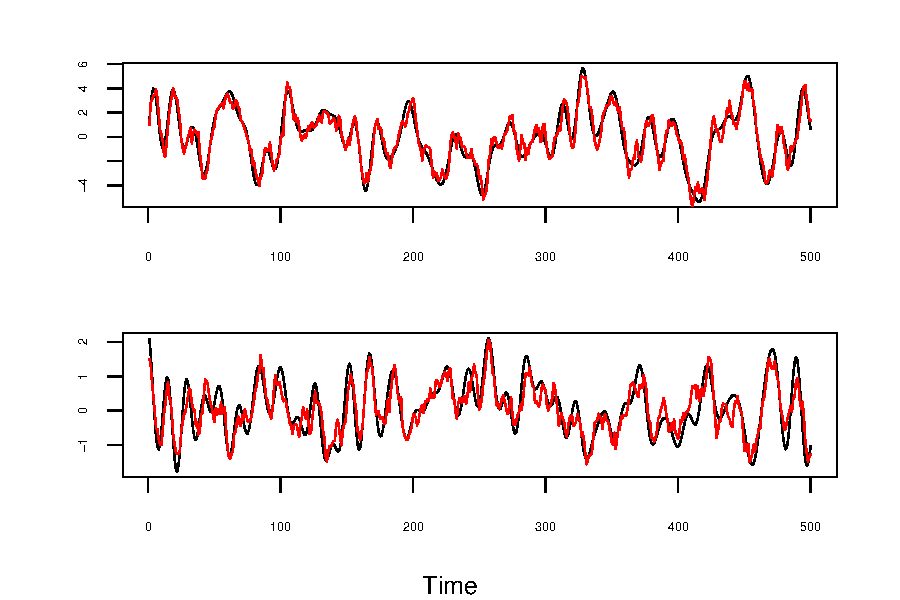
\includegraphics[]{mdfa_var1_filtering.pdf}
\caption{Ideal trends (black) for the bivariate VAR(1)
	with real-time MDFA trends (grey) overlaid, for series one (upper panel)
	and series two (bottom panel).}
\label{fig:var1.trends}
\end{center}
\end{figure}

 Figure \ref{fig:var1.trends} shows the tracking of the ideal trends
 by the MDFA real-time trends.
The MDFA criterion  attempts to find a real-time filter $\widehat{\Psi}$
 that is close to the target $\Psi$ at frequencies that are emphasized
 by spectral content in the time series, which is assessed
 through the periodogram.   This particular 
optimization concept can be understood 
  by analyzing real-time filter outputs and filter 
  characteristics, i.e., amplitude and phase delay functions.


\begin{Exercise} {\bf MDFA VAR(1) Filtering Characteristics.} \rm
\label{exer:var1mdfa2.filter}
 This exercise examines MDFA applied to the trend of a trivariate VAR(1) process,
 which is essentially three univariate AR(1) processes.
Simulate a sample of size $T=5000$ from a
 trivariate VAR(1) process with 
\[
  \Phi = \left[ \begin{array}{ccc} 9/10 & 0 & 0 \\  0 & 1/10 & 0  \\ 0 & 0 & -9/10
   \end{array} \right]
\]
 and $\Sigma$ equal to the identity.   
  Apply the   ideal low-pass filter  with 
  $\mu = \pi/6$ to the sample (truncate the filter to $1000$ coefficients on each side).  
 Use the moving average filter
 MDFA  (Proposition \ref{prop:mdfa.quadsoln}) to find the best
 concurrent filter, setting $q= 12$.  Apply this concurrent filter 
 to the simulation, and compare the relevant portions to the ideal trend.
Also determine the in-sample performance, in comparison to the criterion value
 (\ref{eq:opt.val.mdfa}).
  Target the trends for both time series, and compare the results graphically.
 Finally, compute and graphically compare  the amplitude and phase delay
   functions for each of the three trend targets.
\end{Exercise}


\begin{Schunk}
\begin{Sinput}
> # Simulate a Gaussian VAR(1) of sample size 2500:
> set.seed(1234)
> T <- 5000
> N <- 3
> phi.matrix <- rbind(c(.9,0,0),c(0,.1,0),c(0,0,-.9))
> innovar.matrix <- diag(N)
> true.psi <- var.par2pre(array(phi.matrix,c(N,N,1)))
> gamma <- VARMAauto(array(phi.matrix,c(N,N,1)),NULL,innovar.matrix,10)
> gamma.0 <- gamma[,,1]
> x.init <- t(chol(gamma.0)) %*% rnorm(N)
> x.next <- x.init
> x.sim <- NULL
> for(t in 1:T)
+ {
+ 	x.next <- phi.matrix %*% x.next + t(chol(innovar.matrix)) %*% rnorm(N)
+ 	x.sim <- cbind(x.sim,x.next)
+ }
> x.sim <- ts(t(x.sim))
> x.acf <- acf(x.sim,type="covariance",plot=FALSE,lag.max=T)[[1]]
> x.acf <- aperm(aperm(x.acf,c(3,2,1)),c(2,1,3))
> # construct and apply low pass filter
> mu <- pi/6
> len <- 1000
> lp.filter <- c(mu/pi,sin(seq(1,len)*mu)/(pi*seq(1,len)))
> lp.filter <- c(rev(lp.filter),lp.filter[-1])
> x.trend.ideal <- filter(x.sim,lp.filter,method="convolution",sides=2)[(len+1):(T-len),]
> # get MDFA concurrent filter
> q <- 20
> grid <- T
> m <- floor(grid/2)
> # The Fourier frequencies
> freq.ft <- 2*pi*grid^{-1}*(seq(1,grid) - (m+1))
> # frf for ideal low-pass
> frf.psi <- rep(0,grid)
> frf.psi[abs(freq.ft) <= mu] <- 1
> frf.psi <- matrix(frf.psi,nrow=1) %x% diag(N) 	  
> frf.psi <- array(frf.psi,c(N,N,grid))
> spec.hat <- mdfa.pergram(x.sim,1)	
> lp.mdfa <- mdfa.unconstrained(frf.psi,spec.hat,q)
> # apply the MDFA concurrent filter
> x.trend.mdfa <- mvar.filter(x.sim,lp.mdfa[[1]])[(len-q+2):(T-q+1-len),]
> # compare in-sample performance
> print(c(mean((x.trend.ideal[,1] - x.trend.mdfa[,1])^2),
+ 	mean((x.trend.ideal[,2] - x.trend.mdfa[,2])^2),
+ 	mean((x.trend.ideal[,3] - x.trend.mdfa[,3])^2)))
\end{Sinput}
\begin{Soutput}
[1] 0.29370453 0.08167332 0.02267826
\end{Soutput}
\begin{Sinput}
> # compare to criterion value
> diag(lp.mdfa[[2]])
\end{Sinput}
\begin{Soutput}
[1] 0.30165107 0.08364418 0.02316804
\end{Soutput}
\begin{Sinput}
> # compute gain and phase delay functions
> frf.psi <- frf.psi[1,1,]
> gain.psi <- abs(frf.psi)
> phased.psi <- Arg(frf.psi)/freq.ft
> lp.frf <- mdfa.frf(lp.mdfa[[1]],0,T)
> lp.gain1 <- abs(lp.frf[1,1,])
> lp.gain2 <- abs(lp.frf[2,2,])
> lp.gain3 <- abs(lp.frf[3,3,])
> lp.phased1 <- -Arg(lp.frf[1,1,])/freq.ft
> lp.phased2 <- -Arg(lp.frf[2,2,])/freq.ft
> lp.phased3 <- -Arg(lp.frf[3,3,])/freq.ft
\end{Sinput}
\end{Schunk}


\begin{figure}[htb!]
\begin{center}
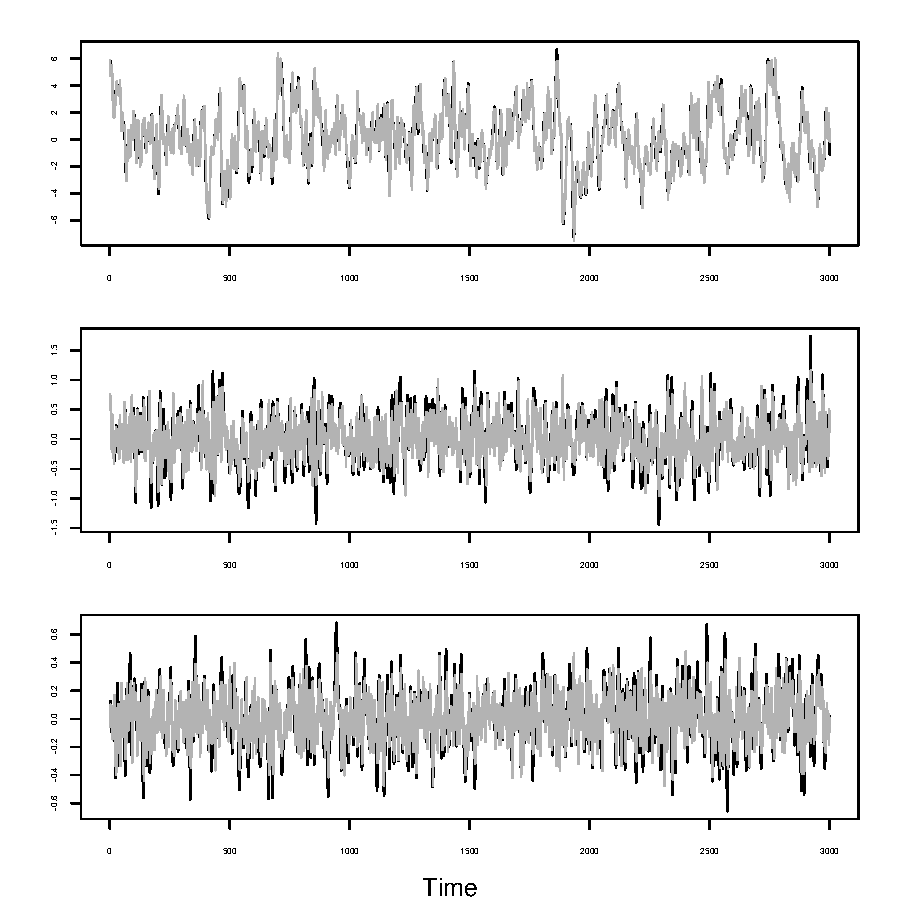
\includegraphics[]{mdfa_trivar1_filtering.pdf}
\caption{Ideal trends (black) for the trivariate VAR(1)
	with real-time MDFA trends (grey) overlaid, for series one (upper panel),
	series two (center panel), and series three (bottom panel).}
\label{fig:trivar1.trends} 
\end{center}
\end{figure}


\begin{figure}[htb!]
\begin{center}
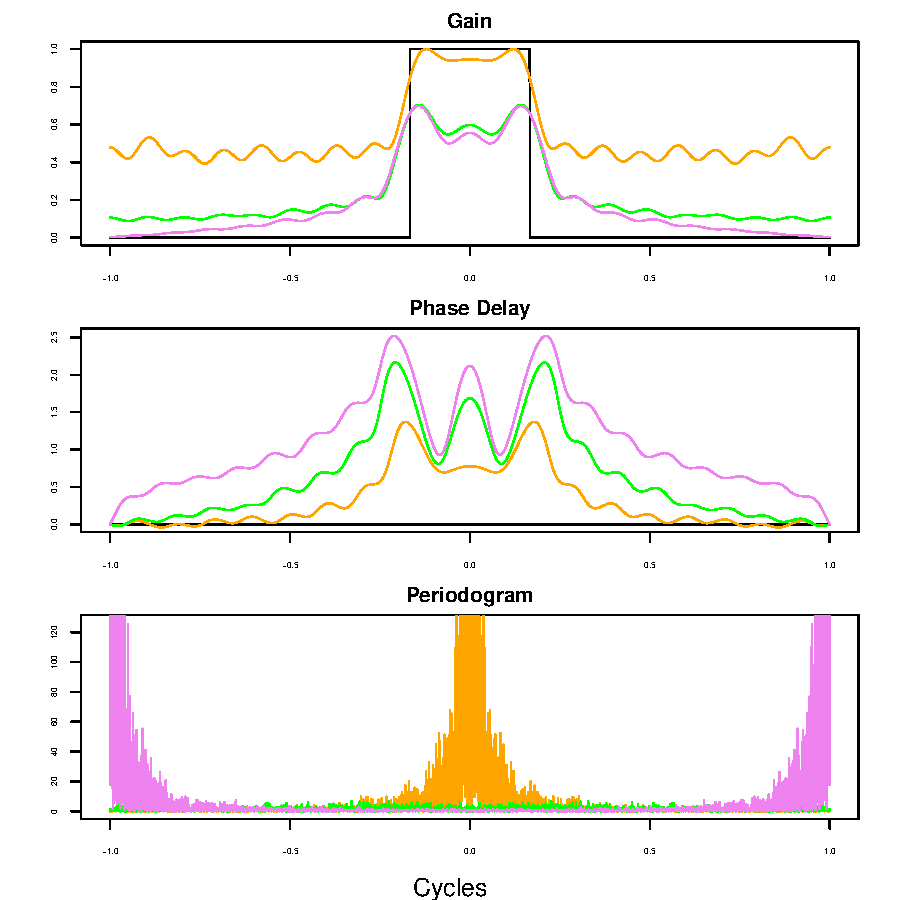
\includegraphics[]{mdfa_trivar1_freqdomain.pdf}
\caption{Gain functions (upper panel), 
	Phase Delay Functions (center panel), and Periodograms (bottom panel)
	 for series one (orange), two (green), and three (violet).}
\label{fig:trivar1.freqdomain}
\end{center}
\end{figure}

 
A visual inspection of Figure \ref{fig:trivar1.trends}, regarding
the trends and trend estimates in Exercise 
 \ref{exer:var1mdfa2.filter}, indicates an apparent conflict with the 
 criterion values: although the first series has the largest MSE,
 the fit of the concurrent estimator to the target trend appears best.
 This is because the task of the filter for the first series is
 easiest, because a higher degree of smoothness must be captured --
 whereas, in contrast, a noisy target is harder to replicate in a
 mean square error sense. Another feature is that the real-time
 estimates appear  to be systematically 
shifted to the right (they are delayed); the first series seems to be least
 affected.   These observations indicate that the difficulty of the estimation 
  task  depends on the DGP (as specified by the entries of $\Phi$):
 larger eigenvalues correspond to greater persistence of the process, 
  and an easier estimation problem.  In contrast, small eigenvalues 
 correspond to a noisier process, and a harder estimation problem.
 
 These properties are further confirmed by the gain and phase delay
 functions displayed   in Figure \ref{fig:trivar1.freqdomain}.   
 The noise  in real-time estimates $\widehat{Y}_t$  
 is due to the incomplete matching of the estimated gain (orange, green, or
 violet lines in the upper panel) to the ideal gain function (black); 
  note that the concurrent
 filters allow some   content at frequencies greater than $\mu = \pi/6$
 to penetrate.  On the other hand, the observed delay in the real-time
 estimates can be explained through the fact that the phase delay functions
 of the concurrent filters (orange, green, or
 violet lines in the center panel) do not vanish, unlike the ideal
 filter's phase delay (black).    Chapter \ref{chap:ats} 
proposes a more general optimization paradigm that will address these issues 
explicitly.

 Also observe that the phase delay function of the first series
 (orange line, center panel), which has the strongest autocorrelation,
  remains comparatively small. Its gain function (orange line, upper panel) 
 is the farthest away from the target in the stop-band $|\omega| >\pi/6$,
   but most closely resembles the target in the pass-band 
	$|\omega| \leq\pi/6$.
  Apparently,  the optimization criterion concedes
 poorer high-frequency damping to obtain improved pass-band properties. 
 In summary, $\widehat{\Psi}$ tracks $\Psi$ towards the pivotal
 frequencies, i.e., those that are important to the process'
 dynamics, as quantified by the periodogram (bottom panel) in 
 Figure \ref{fig:trivar1.freqdomain}.  
Similar findings apply to the other two series.




\section{Qualitative Easing by Leading Indicators: an Empirical Study}
   \label{sec:leading.ind}

In this section we quantify performance gains 
  obtained by inclusion of a leading indicator into a univariate design.
 In particular, consider the process
\begin{align}
 X_{t,1} & = \phi \, X_{t-1,1} + \epsilon_{t,1} \notag \\
 X_{t,2} & = X_{t+\delta,1} + \sigma \, \epsilon_{t,2}, \label{def_led_i}
\end{align} 
  where $\{ \epsilon_t \}$ is i.i.d. with mean zero and identity covariance matrix.
  Clearly, $\{ X_{t,2} \}$ is a leading indicator of $\{ X_{t,1} \}$ when
 the time-shift  $\delta > 0$.   The scaling factor $\sigma$ determines  
 the extent to which the indicator is effective, with 
 larger values of  $\sigma$ implying that the indicator is less 
informative about the target $X_{t,1}$.

\subsection{Bivariate MDFA versus Univariate DFA}
 \label{bimdfaudfa}

Here   we select $\sigma=1$, corresponding to a weak
 idiosyncratic component, and set $\delta=1$ so that the indicator
 leads by one time unit.
 

\begin{Exercise} {\bf Strong Leading Indicator.} \rm
\label{exer:bimdfa-udfa}
 Simulate a sample of size $T=200$ from the process (\ref{def_led_i}) with
 $\phi = .9$, $\delta = 1$, and $\sigma = 1$.  The target is one-step
 ahead forecasting of $\{ X_{t,1} \}$, i.e., $Y_t = X_{t+1,1}$.
  Apply univariate DFA by specializing the MDFA methodology, and compare
 to results obtained from MDFA  (Proposition \ref{prop:mdfa.quadsoln}),
 in each case setting $q=20$.  
  Apply both concurrent filters 
 to the simulation, and compare the relevant portions to the actual
 target.  Also determine the in-sample performance, in comparison to the
   criterion value  (\ref{eq:opt.val.mdfa}), for both the DFA and MDFA methods.
 Compare the results graphically.
\end{Exercise}

\begin{Schunk}
\begin{Sinput}
> # Simulate a Gaussian bivariate process of sample size 200:
> set.seed(1234)
> T <- 200
> N <- 2
> phi <- .9
> sigma <- 1
> gamma.0 <- 1/(1-phi^2)
> x.init <- sqrt(gamma.0)*rnorm(1)
> x.next <- x.init
> x.sim <- x.init
> for(t in 1:T)
+ {
+ 	x.next <- phi * x.next + rnorm(1)
+ 	x.sim <- c(x.sim,x.next)
+ }
> w.sim <- x.sim[-1] + sigma*rnorm(T)
> x.sim <- cbind(x.sim[-(T+1)],w.sim)
> # MDFA
> q <- 20
> grid <- T
> m <- floor(grid/2)
> # The Fourier frequencies
> lambda.ft <- exp(-1i*2*pi*grid^{-1}*(seq(1,grid) - (m+1)))
> # frf for 1-step ahead forecasting
> frf.psi <- matrix(lambda.ft^{-1},nrow=1) %x% diag(N) 	  
> frf.psi <- array(frf.psi,c(N,N,grid))
> spec.hat <- mdfa.pergram(x.sim,1)	
> fore.mdfa <- mdfa.unconstrained(frf.psi,spec.hat,q)
> fore.udfa <- mdfa.unconstrained(frf.psi[1,1,,drop=FALSE],spec.hat[1,1,,drop=FALSE],q)
> # apply the MDFA concurrent filter
> x.fore.mdfa11 <- filter(x.sim[,1],fore.mdfa[[1]][1,1,],method="convolution",sides=1)
> x.fore.mdfa12 <- filter(x.sim[,2],fore.mdfa[[1]][1,2,],method="convolution",sides=1)
> x.fore.mdfa <- x.fore.mdfa11 + x.fore.mdfa12 
> # apply the univariate DFA concurrent filter
> x.fore.udfa <- filter(x.sim[,1],fore.udfa[[1]][1,1,],method="convolution",sides=1)
> # compare in-sample performance
> print(c(mean((x.sim[(q+1):T,1] - x.fore.mdfa[q:(T-1)])^2),
+ 	mean((x.sim[(q+1):T,1] - x.fore.udfa[q:(T-1)])^2)))
\end{Sinput}
\begin{Soutput}
[1] 0.345303 0.934042
\end{Soutput}
\begin{Sinput}
> # compare to criterion value
> print(c(fore.mdfa[[2]][1,1],fore.udfa[[2]][1,1]))
\end{Sinput}
\begin{Soutput}
[1] 0.3437316 0.9552386
\end{Soutput}
\end{Schunk}

 

\begin{figure}[htb!]
\begin{center}
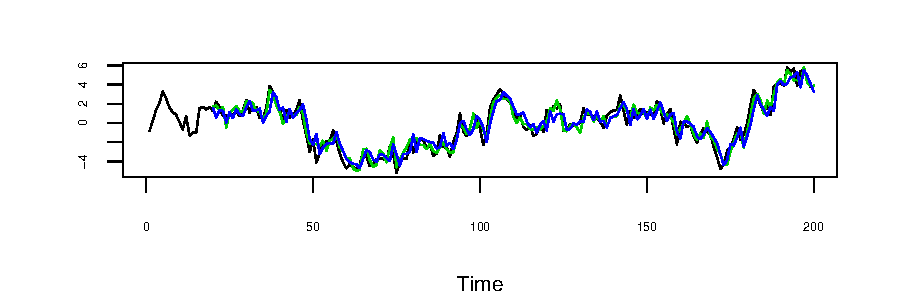
\includegraphics[]{mdfa_bimdfa-udfa.pdf}
\caption{One-step ahead forecasts
 based upon MDFA (black solid) and univariate DFA (dashed dark grey), 
 with target in solid light grey.}
\label{fig:easing1}
\end{center}
\end{figure} 
  

We see that there is a substantial improvement to performance of the MDFA over
 the univariate DFA; this can be visualized by the tracking of the target
 shown in Figure \ref{fig:easing1}.  This is possible because the MDFA filter
 assigns more weight to the second series (the leading indicator), which is
 not available to the univariate DFA.
 

\subsection{Measuring Lead and Signal-to-Noise Effects of a Leading Indicator}
 \label{sec:lead.snr}

Intuitively, increasing $\delta$ or $\sigma$ should result in a harder forecasting
 problem: $1/ \sigma$ measures signal-to-noise ratio (snr), and low values indicate
 that real-time signal extraction becomes more difficult.  On the other hand,
 a high lead time $\delta$ requires one to do long-term forecasting, which is
 known to be hard.
 Through the fabricated  process (\ref{def_led_i}) we can disentangle the conflict
 between increasing $\delta$ and decreasing $\sigma$.
  By allowing for  non-integer shifts $\delta_j=j/4$, $j=0,1,2,3,4$
 we can quantify real-time forecasting performance.  Note
 that if the time units are annual, then the $\delta_j$ correspond to quarterly
 forecasts; more generally, taking $\delta < 1$ corresponds to now-casting
 of a time series, and has many practical applications.
  The target filter has frequency response function of the form
\[
 \Psi (e^{-i \omega}) = \exp \{ i \, \omega \delta \},
\]
 which can be immediately   implemented in the frequency domain
 (whereas in time domain, the filter is difficult to express
 when $\delta$ is non-integer).
 

\begin{Exercise} {\bf Now-casting with a Leading Indicator.} \rm
\label{exer:nowmdfa-udfa}
 Simulate a sample of size $T=2500$ from the process (\ref{def_led_i}) with
 $\phi = .9$, $\delta_j=j/4$, $j=0,1,2,3,4$ and 
$\sigma = 0,0.1,0.5,1,2$.  The target is $\delta$-step
 ahead nowcasting of $\{ X_{t,1} \}$, i.e., $Y_t = X_{t+\delta,1}$.
 Filter to obtain the now-cast target, so as to retain a target series
 of length $500$.  Combine with the leading indicator, and 
  apply univariate DFA and MDFA methodology (Proposition \ref{prop:mdfa.quadsoln}),
 in each case setting $q=20$.  
  Apply both concurrent filters 
 to the simulation, and compare the relevant portions to the actual
 target.  Record the criterion values  (\ref{eq:opt.val.mdfa})
 for both the DFA and MDFA methods.
\end{Exercise}

\begin{Schunk}
\begin{Sinput}
> # Set up loops over delta and sigma
> delta.vals <- c(0,1,2,3,4)/4
> sigma.vals <- c(0,.1,.5,1,2)
> critmdfa.mat <- matrix(0,5,5,dimnames=list(c(0,1,2,3,4)/4,sigma.vals))
> critudfa.mat <- matrix(0,5,5,dimnames=list(c(0,1,2,3,4)/4,sigma.vals))
> for(delta in delta.vals) {
+ for(j in 1:5) {
+ 
+ sigma <- sigma.vals[j]
+ # Simulate a Gaussian bivariate process of sample size 2500:
+ set.seed(1234)
+ T <- 2500
+ N <- 2
+ phi <- .9
+ gamma.0 <- 1/(1-phi^2)
+ x.init <- sqrt(gamma.0)*rnorm(1)
+ x.next <- x.init
+ x.sim <- x.init
+ for(t in 1:T)
+ {
+ 	x.next <- phi * x.next + rnorm(1)
+ 	x.sim <- c(x.sim,x.next)
+ }
+ 
+ grid <- T
+ m <- floor(grid/2)
+ # define complex exponential at Fourier frequencies
+ lambda.ft <- exp(-1i*2*pi*grid^{-1}*(seq(1,grid) - (m+1)))
+ # frf for delta-step ahead forecasting
+ frf.psi <- matrix(lambda.ft^{-delta},nrow=1) 
+ frf.psi <- array(frf.psi,c(1,1,grid))
+ nowcast.filter <- mdfa.coeff(frf.psi,-len,len)
+ x.target <- filter(x.sim,nowcast.filter[1,1,],method="convolution",sides=2)[(len+1):(T-len)]
+ w.sim <- x.target + sigma*rnorm(T-2*len)
+ x.sim <- cbind(x.sim[(len+1):(T-len)],w.sim)
+ 
+ # MDFA
+ q <- 20
+ grid <- T - 2*len
+ m <- floor(grid/2)
+ # The Fourier frequencies (recompute with smaller sample size)
+ lambda.ft <- exp(-1i*2*pi*grid^{-1}*(seq(1,grid) - (m+1)))
+ # frf for delta-step ahead forecasting
+ frf.psi <- matrix(lambda.ft^{-delta},nrow=1) %x% diag(N)
+ frf.psi <- array(frf.psi,c(N,N,grid))
+ spec.hat <- mdfa.pergram(x.sim,1)	
+ fore.udfa <- mdfa.unconstrained(frf.psi[1,1,,drop=FALSE],spec.hat[1,1,,drop=FALSE],q)
+ if(j > 1) { 
+ 	fore.mdfa <- mdfa.unconstrained(frf.psi,spec.hat,q) 
+ } else { fore.mdfa <- fore.udfa }
+   
+ # apply the MDFA concurrent filter
+ x.fore.mdfa11 <- filter(x.sim[,1],fore.mdfa[[1]][1,1,],method="convolution",sides=1)
+ if(j > 1) { 
+ 	x.fore.mdfa12 <- filter(x.sim[,2],fore.mdfa[[1]][1,2,],method="convolution",sides=1) 
+ } else { x.fore.mdfa12 <- 0*x.fore.mdfa11 }
+ x.fore.mdfa <- x.fore.mdfa11 + x.fore.mdfa12 
+ 
+ # apply the univariate DFA concurrent filter
+ x.fore.udfa <- filter(x.sim[,1],fore.udfa[[1]][1,1,],method="convolution",sides=1)
+ 
+ # compare in-sample performance
+ #print(c(mean((x.target[-seq(1,q-1)] - x.fore.mdfa[-seq(1,q-1)])^2),
+ #	mean((x.target[-seq(1,q-1)] - x.fore.udfa[-seq(1,q-1)])^2)))
+ 
+ # store criterion value
+ i <- delta*4 + 1
+ critmdfa.mat[i,j] <- fore.mdfa[[2]][1,1]
+ critudfa.mat[i,j] <- fore.udfa[[2]][1,1]
+ }}
\end{Sinput}
\end{Schunk}

% OLD way of generating table
%xtb <- xtable(critmdfa.mat, dec = 1,digits=rep(3,dim(critmdfa.mat)[2]+1),
%  paste("Effect of lead and  inverse signal-to-noise ratio on MDFA filter MSE",sep=""),
%  label=paste("tab:critmdfa.mat",sep=""),
%  center = "centering", file = "", floating = FALSE)
%addtorow <- list()
%addtorow$pos <- list(-1)
%addtorow$command <- paste0(paste0('$','\\','delta$','& \\multicolumn{5}{c}{Sigma values}', %collapse=''), '\\\\')
%print(xtb, add.to.row=addtorow, include.colnames=T)
%
%xtb <-  xtable(critudfa.mat, dec = 1,digits=rep(3,dim(critudfa.mat)[2]+1),
%  paste("Effect of lead and  inverse signal-to-noise ratio on DFA filter MSE",sep=""),
%  label=paste("tab:critudfa.mat",sep=""),
%  center = "centering", file = "", floating = FALSE)
%addtorow <- list()
%addtorow$pos <- list(-1)
%addtorow$command <- paste0(paste0('$','\\','delta$','& \\multicolumn{5}{c}{Sigma values}', %collapse=''), '\\\\')
%print(xtb, add.to.row=addtorow, include.colnames=T)

\begin{table}[]
\centering
\caption{Effect of lead and  inverse signal-to-noise ratio on MDFA filter MSE.}
\label{tab:critmdfa.mat}
\begin{tabular}{llllll}
  & 0    & 0.25   & 0.5  
   & 0.75  & 1  \\ \hline
0        & -3.5527136788005e-15  & 2.22044604925031e-13 
    & -1.77635683940025e-15 & -8.88178419700125e-16 & 3.5527136788005e-15  \\
0.1        & 0.0515333063544694  & 0.00927538700613129 
    & 0.0347401278748989 & 0.0435319652609754 & 0.047145822050028  \\
0.5        & 0.24160844893295  & 0.0240008079865022 
    & 0.100443415264753 & 0.164859934734334 & 0.204834451331773  \\
1        & 0.54284235518345  & 0.0398437844476653 
    & 0.157774326108716 & 0.305402560379077 & 0.427518962824753  \\
2        & 0.857285264133202  & 0.0505989535031648 
    & 0.19502275802409 & 0.414781672651307 & 0.635241666441922  \\
\hline      
\end{tabular}
\end{table}
 
 
 \begin{table}[]
\centering
\caption{Effect of lead and  inverse signal-to-noise ratio on DFA filter MSE.}
\label{tab:critudfa.mat}
\begin{tabular}{llllll}
  & 0    & 0.25   & 0.5  
   & 0.75  & 1  \\ \hline
0        & -3.5527136788005e-15  & -3.5527136788005e-15 
    & -3.5527136788005e-15 & -3.5527136788005e-15 & -3.5527136788005e-15  \\
0.1        & 0.0515333063544694  & 0.0515333063544694 
    & 0.0515333063544694 & 0.0515333063544694 & 0.0515333063544694  \\
0.5        & 0.24160844893295  & 0.24160844893295 
    & 0.24160844893295 & 0.24160844893295 & 0.24160844893295  \\
1        & 0.54284235518345  & 0.54284235518345 
    & 0.54284235518345 & 0.54284235518345 & 0.54284235518345  \\
2        & 0.857285264133202  & 0.857285264133202 
    & 0.857285264133202 & 0.857285264133202 & 0.857285264133202  \\
\hline      
\end{tabular}
\end{table}

 The results for MDFA and univariate DFA, respectively, are given in 
Tables \ref{tab:critmdfa.mat} and \ref{tab:critudfa.mat}.
Regarding the design of Exercise \ref{exer:nowmdfa-udfa}, we make the following 
comments.  When $\sigma = 0$ the leading indicator exactly matches the target;
 if $\delta = 0$ as well, then $X_{t,1} = X_{t,2}$ and there is redundancy in
 the data -- this will lead to a singularity in the periodogram.  When 
 $\delta > 0$ (but $\sigma = 0$) then $\{ X_{t,1} \}$ and $\{ X_{t,2} \}$
 are perfectly coherent, as the relation $X_{t,2} = B^{-\delta} \, X_{t,1}$ holds.
 This full coherency indicates a type of redundancy is still present,
 and the MDFA method is singular.  Therefore, in these cases we restrict
 the MDFA to univariate DFA.  Therefore, the first columns of 
 Tables \ref{tab:critmdfa.mat} and \ref{tab:critudfa.mat} are identical.

 The first rows of Tables \ref{tab:critmdfa.mat} and \ref{tab:critudfa.mat}
 are trivially zero, because when $\delta = 0$ the target is observable,
 and hence both MDFA and DFA select the identity filter.  
 Broadly, the patterns are what we would expect: increasing $\delta$ and/or
 $\sigma$ generates worse performance (higher MSE), although the MDFA is
 superior to DFA.  The performance of MDFA relative to DFA worsens as 
 $\sigma$ increases, irrespective of $\delta$, which makes sense: there
 is less benefit to the leading indicator when the snr is low, in which
 case DFA should generate a competitive real-time filter.
  In particular, reading across the rows of Table \ref{tab:critudfa.mat}
 we see the MSE is fairly constant -- DFA does not utilize the leading indicator,
 so the variability here is due to the simulation seeds.
  As for the MDFA, decreased performance due to lower snr could be 
 compensated by decreasing the lead-time $\delta$.  
  Again, when $\sigma$ is low (second column of Table \ref{tab:critmdfa.mat})
  the leading indicator is very useful, and the MSE does not depend 
 greatly on $\delta$.  This pattern is opposite when $\sigma$ is high 
 (fifth column), as increased $\delta$ deleteriously affects performance.

   
These results suggest the pertinence of a mixed-frequency approach,
 whereby information at differing sampling frequencies (such as monthly
 and quarterly data) is combined.  The higher-frequency data stream
 could be used to update the filter for the lower-frequency time series;
 this is further discussed in Chapter \ref{chap:mix}. 
 


\section{Multivariate DFA with Multiple Targets}
 
  
 We now consider a slight generalization of the LPP, where the target is also multivariate.
 
\subsection{LPP with Multiple Targets} 
 
\begin{Definition} \rm
\label{def:target2}
 A {\bf target} is defined to be the output of any known linear
 filter acting on the data process, i.e.,  $\{Y_t \}$ is a target
 time series corresponding to a given filter $\Psi (L)$ acting on a 
given observed time series
 $\{ X_t \}$ if and only if we can write $ Y_t = \Psi (L) \, X_t$
 for all integers $t$.
\end{Definition}

 We revisit the examples considered in Chapter \ref{lpp_chap}, but
 now incorporated with multiple targets.

\begin{Example} {\bf  Multi-step Ahead Forecasting.}   \rm
\label{exam:multi-step.fore2}
  Suppose that our goal is to forecast all of the component series 
 $h$ steps ahead, where $h \geq 1$ is the given {\em forecast lead}.
  Hence the target is expressed as  $  Y_t = X_{t+h}$
  for all $ t \in \ZZ$.  This target corresponds to
  $\Psi (L) = L^{-h} \, 1_n$.   Thus,   $\psi (\ell)$  is a $n \times n$
  matrix, each of which are zero except $\psi (-h)$,
 which is given by $1_n$.
\end{Example}

\begin{Example} {\bf Ideal Low-Pass.} \rm
\label{exam:ideal-low2}
  The ideal low-pass target is the same for each series, and hence
\[
  \Psi (z) = \chi_{ [ -\mu, \mu ]} (\omega) \,1_n
\]
 for some cutoff $\mu \in (0, \pi)$ that separates the pass-band from
the stop-band.   The coefficients are given by 
\[ 
  \psi (\ell) = \frac{ \sin (\ell \mu) }{ \pi \ell } \, 1_n
\]
 for $\ell \neq 0$ and $\psi (0) = \mu/\pi \, 1_n$.   
\end{Example}

\begin{Example} {\bf The Future VAR(1) Shock.}\rm
\label{exam:var1-shock}
  Consider the VAR(1) process (\ref{eq:var1-def}), and suppose our target is the future shock
  (or innovation), so that
\[
  Y_t = X_{t+1} - \Phi \, X_{t}.
\]
  Hence $\Psi (L) = L^{-1} 1_n - \Phi$.  Note that this target is model-based;
  one must know the process to compute the target.   Also, each component of
  the multivariate target depends on all the series:
\[
  Y_{t,j} = X_{t+1,j} -  \sum_{k=1}^n \Phi_{jk} X_{t,k}
\]
 for $1 \leq j \leq n$.
\end{Example}

As we see from these examples, the targets of real-time signal 
 extraction  are features of the stochastic process that are of interest to 
 a particular user.   Targets can be {\em ad hoc} 
 (cf. Example \ref{exam:ideal-low}2) or {\em model-based} (cf. Example \ref{exam:var1-shock}),
   and may   depend upon  all the components   of $X_t$.    
 

\begin{Definition} \rm
\label{def:lpp2}
 The {\bf Linear Prediction Problem} (LPP) seeks a linear estimate
    such that the filter error (\ref{eq:dfa-error})
 has mean zero, and  such that the determinant of the filter 
    error variance $\mbox{Var} [ E_t ]$ is minimized.
\end{Definition}

The filter error variance matrix is referred to as the filter MSE;
 the diagonal entries correspond to the scalar LPPs considered
 earlier in this book.   We now state the   solution to the general LPP
 with multiple targets.

\begin{Proposition}
 \label{prop:GPP2}
 Suppose that $\{ X_t \}$ is mean zero and weakly stationary 
 with  causal Wold decomposition expressed as $X_t = \Theta (L) \, \epsilon_t$,
 where $\Theta (L)$ is invertible.    Then the solution
 to the LPP posed by a   target $Y_t = \Psi (L) \, X_t$ is given by
\begin{equation}
 \label{eq:GPPsoln}
 \widehat{\Psi} (L) = \sum_{\ell \geq 0 } \psi (\ell) \, L^{\ell} + 
 \sum_{\ell < 0 } \psi (\ell)
 \,  { [ \Theta (L) ]}_{-\ell}^{ \infty  } \, L^{\ell} \, {\Theta (L) }^{-1}.
\end{equation}
 Moreover, the   MSE  corresponding to this solution is given by
\begin{equation} 
\label{eq:minimalMSE}
 \frac{1}{ 2 \pi} \int_{-\pi}^{\pi}   \sum_{\ell, k > 0 } \psi (-\ell) \,
  {[ \Theta  (e^{-i \omega}) ]}_0^{\ell-1}   \,  \Sigma \,
  { {[ \Theta  (e^{i \omega}) ]}_0^{ k-1} }^{\prime}  \,
   {\psi (-k) }^{\prime} \,  e^{i \omega (\ell - k) }   \, d\omega.
\end{equation}
 \end{Proposition}

  

\paragraph{Proof of Proposition \ref{prop:GPP2}.}
 In order for a linear solution to be MSE optimal, it is sufficient that the
 resulting error process be uncorrelated with the present and past data, denoted $X_{t:}$.
   If we can show that the real-time signal extraction error process $\{ E_t \}$
  depends only on future innovations, then by the causality of $\{ X_t \}$ the error process 
  must be uncorrelated   with $X_{t:}$, establishing optimality.  
 The filter error of the putative solution is  
  given by
\begin{align*}
 \Psi (L) - \widehat{\Psi} (L) & = \sum_{\ell < 0 } \psi (\ell) \, L^{\ell} \,
   \left( 1 -   {[ \Theta (L) ]}_{-\ell}^{\infty} \, { \Theta (L) }^{-1} \right) \\
  & =  \sum_{\ell < 0 } \psi (\ell) \, L^{\ell} \, 
  {[ \Theta (L) ]}_{0}^{ -(\ell + 1)} \, { \Theta (L) }^{-1}.
\end{align*}
 Applying this to $\{ X_t \}$ yields
\[
  E_t = \sum_{\ell =1 }^{\infty} \psi (-\ell) \, {[ \Theta (L) ]}_0^{\ell - 1} \, 
   \epsilon_{t + \ell }.
\]
  Noting that ${[ \Theta (L) ]}_0^{\ell - 1}$ is an order $\ell-1$ polynomial in $L$,
 and is applied to $\epsilon_{t+ \ell}$, it is apparent that $E_t$ is a linear function
 of future innovations $\{ \epsilon_{t+1}, \epsilon_{t+2}, \ldots \}$.  Computing
 the variance of $E_t$ yields the expression for the minimal MSE.  $\quad \Box$

 
\subsection{MDFA for Multiple Targets}

Suppose that the causal filters of interest belong to a class
  $\mathcal{G}$  described by a vector parameter $\vartheta$ belonging to a 
 parameter manifold.  We now generalize the definition of $\mathcal{G}$ given
  by (\ref{eq:filter-set}),  where now the filters are $n \times n$.
  Likewise, we generalize the real-time estimation error   given in (\ref{eq:dfa-error})
 by noting that now $E_t$ is an $n$-dimensional vector.  
  Hence (\ref{eq:dfa-mvar}) becomes
\begin{equation}
 \label{eq:dfa-mvar2}
   \EE [ \varepsilon_t \, \varepsilon_t^{\prime} ]  = 
   { \langle  \left[ \Psi ( e^{-i \omega} ) -  
   \widehat{\Psi}_{\vartheta} (e^{-i \omega}) \right] \,   F (\omega) \,
  {  \left[ \Psi (e^{i \omega}) -  \widehat{\Psi}_{\vartheta} (e^{i \omega}) \right] }^{\prime} \rangle }_0.
\end{equation}
   This suggests as a generalization of (\ref{eq:mdfa-criterion})
   the criterion function  $\det D_{\Psi} (\vartheta, G)$ for
 any Hermitian function $G$, defined via
\begin{equation}
\label{eq:mdfa-criterion2}
 D_{\Psi} (\vartheta, G) = { \langle  \left[ \Psi (e^{-i \omega}) - 
  \widehat{\Psi}_{\vartheta} (e^{-i \omega}) \right] \,   G (\omega) \,
  {  \left[ \Psi (e^{i \omega}) -  \widehat{\Psi}_{\vartheta} (e^{i \omega}) \right] }^{\prime} \rangle }_0.
\end{equation}
  In the following development, setting $G = F$ yields an ideal criterion based on the process,
 whereas setting $G =  \widehat{F}$ (the periodogram) yields an empirical criterion,
 providing estimates  that we can compute from data.  
 Taking the determinant of (\ref{eq:mdfa-criterion2}) yields
 the MDFA criterion function.   In the case $n=1$ we recover the univariate DFA; 
 Proposition A.3 of McElroy and Wildi (2020)  shows
that by including additional time series the MDFA will  improve over DFA for any filter class $\mathcal{G}$.

The  best possible concurrent filter is  given by
 $\widehat{\Psi}_{\vartheta (F)}$,
  where $\vartheta (F)$ is a minimizer of
  $\det D_{\Psi} (\vartheta, F)$.  This $\vartheta (F)$ is the
 Pseudo-True Value  for the filter parameter.
A   case of interest arises from taking a very broad class $\mathcal{G}$, namely
  let $\mathcal{G}$ consist of all length $q$ concurrent filters, with 
$\vartheta =  \mbox{vec} [\Xi^{\prime}]$ and 
\begin{equation}
\label{eq:conc.filter}
  \Xi^{}  =  {\left[  \widehat{\psi} (0), \widehat{\psi} (1), \ldots, 
  \widehat{\psi} (q-1) \right] }^{\prime}.
\end{equation}
 So $\Xi$ is  a   $ q n \times n$ dimensional matrix.
 Then the criterion (\ref{eq:mdfa-criterion2}) can be rewritten as
\begin{equation}
\label{eq:mdfa-crit.linear}
 D_{\Psi} (\vartheta, G)  = \Xi^{\prime} \, B \, \Xi -
   \Xi^{\prime} \, A - 
   A^{\prime} \, \Xi + { \langle \Psi (e^{-i \omega}) \, G (\omega) \, { \Psi (e^{i \omega}) }^{\prime} \rangle }_0,
\end{equation}
 where 
\begin{equation}
 \label{eq:bstar-expression}
  A^{\prime}  = \left[ { \langle \Psi (e^{-i \omega}) \, G (\omega) 
  \rangle }_{0}, { \langle \Psi (e^{-i \omega}) \, G (\omega) \rangle }_{1},
  \ldots, { \langle \Psi (e^{-i \omega}) \, G (\omega) \rangle }_{q-1} \right],
\end{equation}
  and $B$ is a block matrix such that  the $jk$th $n \times n$ block of $B$  is 
  ${ \langle G \rangle }_{k-j}$ for $1 \leq j,k \leq q$.  (Because $G$ is Hermitian,
 ${ \langle G \rangle }_{k-j}$ is real, and it follows that $A$ is real as well.)



\begin{Proposition}
\label{prop:mdfa.quadsoln2}
 The minimizer of the   MDFA criterion given by the determinant of (\ref{eq:mdfa-criterion2}),
  with respect to $\mathcal{G}$ consisting of all length $q$ concurrent filters,  is
  $ \Xi (G) = B^{-1} \, A$,
 where the $jk$th  block of $B$   is    ${ \langle G \rangle }_{k-j}$,
 and $A$ is given by (\ref{eq:bstar-expression}).
 The minimal value is the determinant of
\begin{equation}
\label{eq:opt.val.mdfa2}
{ \langle \Psi (e^{-i \omega}) \, G (\omega) \, { \Psi (e^{i \omega}) }^{\prime} \rangle }_0 - A^{\prime} \, B^{-1} \, A.
\end{equation}
\end{Proposition}

\paragraph{Proof of Proposition \ref{prop:mdfa.quadsoln2}.}
 First note that the typical component of $A$ has the form
\begin{equation}
 \label{eq:psi.g.comp2}
   { \langle \Psi (z) \, G \rangle }_{\ell} = \sum_{k = - \infty}^{\infty} \psi (k) \,
	 { \langle G \rangle }_{\ell-k}
\end{equation}
 for $0 \leq \ell < q$,  which shows that $A$ is real-valued. 
 The argument follows the same method as in McElroy and Findley (2015);
 each entry of the matrix objective function is a quadratic in $\Xi$, and therefore
  the minimizer is obtained 
 by computing the gradient and Hessian, which are 
  $-2 A + 2 B \, \Xi$ and   $2 B$ respectively,
  yielding the solution.  Plugging back into $D_{\Psi}$ yields (\ref{eq:opt.val.mdfa2}).
$\quad \Box$


 
\begin{Example} {\bf One-step Ahead Forecasting.}  \rm
\label{exam:multi-step.fore.4-alt}
 We now generalize the result of Example \ref{exam:multi-step.fore.4} by considering
  multiple series at once.   Consider the   one-step ahead forecasting of 
  stationary time series, where 
 $\mathcal{G} $ corresponds to   all VMA filters of   order $q$
  (i.e., the filter corresponds to a VMA($q-1$) polynomial), where  
 $ \vartheta  = \mbox{vec} [{\widehat{\psi} (0) }^{\prime},
 {\widehat{\psi} (1) }^{\prime},   \ldots,
  {\widehat{\psi} (q-1) }^{\prime} ]$.
 With $\Psi (z) = z^{-1} 1_n$, from (\ref{eq:mdfa-criterion2}) we have 
\begin{align*}
 D_{\Psi} (\vartheta, G) & = 
 { \langle  \left[  e^{i \omega} 1_n -  \widehat{\Psi}_{\vartheta} (e^{-i \omega}) \right] \,   G (\omega) \,
  {  \left[ e^{-i \omega}  1_n  -  \widehat{\Psi}_{\vartheta} (e^{i \omega}) \right] }^{\prime} \rangle }_0 \\
 & = { \langle  \left[ 1_n -  \sum_{\ell = 0}^{q-1} \widehat{\psi} (\ell)
    \, e^{-i \omega  (\ell+1) } \right] \, 
  G \,   {  \left[ 1_n  -   \sum_{\ell = 0}^{q-1} \widehat{\psi} (\ell) 
  \, e^{i \omega (\ell+1 ) } \right]
  }^{\prime} \rangle }_0 \\
 & = { \langle G \rangle }_0 - 2 \, \Xi^{\prime} \, { \langle G \rangle }_{1:q} 
    + \Xi^{\prime} \, B \, \Xi.
\end{align*}
 Hence the  optimizer is   $ \Xi (G) = B^{-1} \,    { \langle G \rangle }_{1:q}$,
 which is the first component of the solution to the Yule-Walker system of order 
  $q$ determined by $G$.
  Therefore the MDFA solution is the same as the fit of a VAR($q$) using 
 Proposition \ref{prop:GPP2}.
\end{Example}
 

 
  We designate the resulting   prediction function
$\widehat{\Psi}_{ {\vartheta} (G)}$  as  a {\em Linear
Prediction Filter} (LPF).   Again, when $G=F$ this LPF is a theoretical
 object, but when $G = \widehat{F}$ the LPF can be constructed directly from the sample.
  When $\mathcal{G}$ is large enough to include the optimal MB filter
 $\widehat{\Psi}  $ of Proposition  \ref{prop:GPP2},  then
 $\widehat{\Psi}_{ {\vartheta} (F)} $ corresponds to  this 
 $\widehat{\Psi}$ (assuming  the model 
 is correctly specified).
 
  

\begin{Illustration} {\bf VAR($1$).}  \rm
\label{ill:var1.3-alt}
  We revisit the VAR(1) Illustration \ref{ill:var1.3}.
  Now  the solution given by Proposition \ref{prop:mdfa.quadsoln2}
 can be compared to that of the LPP, which has the first $q$ components
 given by $  \Upsilon^{\prime} = [ \psi (0) + A_{\Psi} (\Phi), \psi (1),
 \ldots, \psi (q-1)  ]$.
 This is an approximate solution to the system $\Xi^{\prime} \, B
 =  A^{\prime}$, because
 $  \Upsilon^{\prime} \, B $ has $j+1$th component, for $0 \leq j \leq q-1$,
 equal to  $   \sum_{\ell=0}^{q-1} \psi (\ell) \, {\langle G \rangle }_{j-\ell}
 + A_{\Psi} (\Phi) \, \Gamma_j$.  Noting that
\[
 A_{\Psi} (\Phi) \, \Gamma_j
 = \sum_{\ell = -1 }^{-\infty} \psi (-\ell) \, \Phi^{-\ell} \, \Gamma_j
 = \sum_{\ell = -1}^{\infty} \psi (-\ell) \, \Gamma_{j- \ell},
\]
 because for a VAR($1$) process $\Gamma_h = \Phi^h \, \Gamma_0$ when
 $h \geq 0$, we see that component $j+1$ of $\Upsilon^{\prime} \, B$ is
\[
  \sum_{\ell =0 }^{ q-1} \psi (\ell) \, \Gamma_{j-\ell}
  =  {[   A^{\prime} ]}_{j+1} - \sum_{\ell = q}^{\infty} \psi (\ell) \, \Gamma_{j-\ell}.
\]
 As $q \tends \infty$ the error term vanishes (for each $j$), indicating
 that $\Upsilon^{\prime} \, B \approx  A^{\prime}$, or
 $\Xi \approx \Upsilon$.
\end{Illustration}
 
 For computation, we update the treatment given earlier to now discuss the 
 case of a multivariate filter output.
To compute the quantities given in Proposition \ref{prop:mdfa.quadsoln2} and  
the MDFA criterion (\ref{eq:mdfa-criterion2}), we 
approximate each integral by an average over Fourier frequencies: 
\[
  T^{-1} \, \sum_{t=1}^T E_t \, E_t^{\prime} =
  T^{-1} \sum_{j=-[T/2]}^{T-[T/2]-1}   \widehat{F}_{E} (\omega_{j}),
\]
 where $  \widehat{F}_{E}$ is the periodogram of the 
 filter errors and $\omega_j = 2 \pi \, j/T $ is
 a Fourier frequency.   The right hand side
 (with $ \widehat{F}_X$ the periodogram of the process)  is approximated  by 
\[
 T^{-1} \sum_{j=-[T/2]}^{T-[T/2]-1}  \left[ \Psi (e^{-i \omega_{j} }) - \widehat{\Psi} (e^{-i \omega_{j} }) \right] \,
     \widehat{F}_X (\omega_{j}) \,
 {\left[ \Psi (e^{i \omega_{j} }) - \widehat{\Psi}( e^{i \omega_{j} }) \right]}^{\prime}.
\]
   This is exactly the   criterion $D_{\Psi} (\vartheta,  \widehat{F}_X)$ of
 (\ref{eq:mdfa-criterion2}) with the integrals replaced by Riemann
 sums over the Fourier frequencies.

With this justification, we see that the entries of the matrix $B$ in 
 Proposition \ref{prop:mdfa.quadsoln2} are approximately computed via
\[
  B_{j,k} \approx T^{-1} \sum_{\ell=-[T/2]}^{T-[T/2]-1} G (\omega_{\ell}) \,
   \exp \{ i \, (k-j) (\omega_{\ell}) \}
\]
 for $1 \leq j,k \leq T$.  Moreover, for $0 \leq k \leq T-1$
\[
  A_k^{\prime} \approx T^{-1}  \sum_{\ell=-[T/2]}^{T-[T/2]-1} \Psi 
	( e^{ -i \omega_{\ell} }) \,     G (\omega_{\ell}) \,
   e^{ i  k \omega_{\ell} },
\]
 where $A^{\prime} = [ A_0^{\prime}, \ldots, A_{T-1}^{\prime} ]$.  Finally,
\[
  { \langle \Psi (e^{-i \omega}) \, G (\omega)  \, { \Psi (e^{i \omega}) }^{\prime} \rangle }_0 \approx
  T^{-1}  \sum_{\ell=-[T/2]}^{T-[T/2]-1}  \Psi 
	( e^{ -i  \omega_{\ell} } ) \,
     G (\omega_{\ell}) \,  {\Psi  ( e^{ i \omega_{\ell} } ) }^{\prime}.
\]
 
 
%  note: MDFA_basic replaces Mean_square

%----------------------------------------

% Chapter 4

\chapter{Multivariate Direct Filter Analysis for Non-stationary Processes}
\label{chap:int}

 We now extend the basic MDFA of Chapter \ref{chap:basic}  by considering
 the method's application to  non-stationary processes.  
 Section \ref{sec:constraint} introduces the idea of filter constraints
arising from time-varying means, a form of non-stationarity.
 This treatment is generalized in Section \ref{sec:non-stat}
  by the definition of non-stationary processes, and theory for the corresponding
   model-based filters is developed.  Finally, the MDFA criterion for
    non-stationary processes is discussed in Section \ref{sec:mdfa-nonstat}.
 

\section{Constrained MDFA}
\label{sec:constraint}

 Various constraints upon the concurrent filter can be envisioned, 
   and imposing such strictures results in  a constrained MDFA. 
   A chief case of interest arises when the 
    data process has a time-varying mean (which is a form of  non-stationarity);
  then it is necessary to impose additional filter constraints -- otherwise
   the filter error will not have mean zero.    To see why, 
   Write $\Delta (L) = \Psi (L) - \widehat{\Psi} (L)$ as the discrepancy filter,
   so that we see  from (\ref{eq:dfa-error})  
   that $\EE [ E_t ] = \Delta (L) \, \EE [ X_t ]$; 
   by Definition \ref{def:lpp}, we require
 that $\EE [ E_t ] = 0$ for any LPP.  
  If $\EE [ X_t] = 0$ then this condition is always satisfied, but
   for most time series of interest the mean will be nonzero, and is typically
    time-varying.  For such cases additional constraints on $\Delta (L)$ must be imposed,
    which implicitly amount to constraints on $\widehat{\Psi} (L)$.
    
\begin{Example}    {\bf Constant Mean.}  \rm
\label{exam:constant.mean}
  If $\EE [ X_t ] = \mu$, some nonzero constant,  then we require $\Delta (1) = 0$.
  This is because the mean of the filter error is
  \[
   \Delta (B) \, \EE [ X_t] = \Delta(B) \, \mu = \sum_j \delta (j) \, \mu =
   \Delta (1) \, \mu,
  \]
  and this is zero only if $\Delta (1) = 0$.  This is called a Level Constraint (LC).
\end{Example}  

\begin{Example}    {\bf Linear Mean.}  \rm
\label{exam:linear.mean}
  Suppose that $\EE [ X_t ] = \mu \, t$, where $\mu$ is a nonzero slope
 of a linear time trend.  Then it is required that  $\partial {\Delta} (1) = 0$
  in addition to the LC,  which is seen as follows:
  \[
   \Delta (B) \, \EE [ X_t] = \Delta(B) \, \mu \, t =   \mu \, \sum_j \delta (j) \, (t-j)
   = \mu \, \left(t \, \sum_j \delta (j) - \sum_j j \,\delta (j) \right)
    = \mu \, t \, \Delta(1) - \mu \, \partial \Delta (1).
  \]
  This mean of the filter error  is zero only if both $\Delta(1)=0$ and
  $\partial \Delta (1)=0$; the latter condition is called the
   Time-Shift Constraint (TSC).  
\end{Example}  

     Hence, for linear means we obtain
 three fundamental types of constraints: LC, TSC, and Level plus 
 Time-Shift Constraint (LTSC), which combines both LC and TSC.
  Using the fact that $\Delta (L) = \Psi (L) - \widehat{\Psi} (L)$,
   these three constaints can be described as follows:
\begin{align*}
 \mbox{LC} : &  \;  \Delta (1) = 0 \quad \mbox{or} \quad \Psi (1) = \widehat{\Psi} (1) \\
 \mbox{TSC} : &  \;   \partial {\Delta} (1) = 0 \quad \mbox{or} \quad 
 \partial {\Psi} (1) = \partial {\widehat{\Psi}} (1)  \\
 \mbox{LTSC} : &  \;  \Delta (1) = 0,  \,  \partial {\Delta} (1) = 0 \quad 
 \mbox{or} \quad \Psi (1) = \widehat{\Psi} (1), \; \partial {\Psi} (1) =
 \partial {\widehat{\Psi}} (1).
\end{align*}
 In the case of  concurrent filters of form  (\ref{eq:conc.filter}), 
 LC is accomplished by demanding that 
  $\sum_{j=0}^{q-1} \widehat{\psi} (j) = \Psi(1)$.   More generally, we consider  linear constraints  formulated via
\begin{equation}
\label{eq:concurrent-constrain}
  \vartheta = R \, \varphi + Q,
\end{equation}
 where $R$ is $n q \times n r$ and $\varphi$ is $n r \times 1$ dimensional, consisting of 
 free parameters; $Q$ is a matrix of constants, and is $n q \times 1$ dimensional.


\begin{Illustration}  {\bf Level Constraint (LC).}   \rm
\label{ill:lc}
 Note that $\sum_{j=0}^{q-1} \widehat{\psi} (j) = \Psi(1)$ implies that
\begin{equation}
\label{eq:lc-gamma0}
 \widehat{\psi} (0) = \Psi(1) - \sum_{j=1}^{q-1} \widehat{\psi} (j).
\end{equation}
 Hence  $ \varphi^{\prime}  = [ \widehat{\psi} (1), \widehat{\psi} (2), \ldots, \widehat{\psi} (q-1) ] $ and
\[
	R  = \left[ \begin{array}{ccc} -1 & \ldots & -1 \\ 1 & 0 & 0 \\
		\vdots & \ddots & \vdots \\ 0 & 0 & 1  \end{array} \right]  \otimes 1_n \qquad
	Q = \left[ \begin{array}{c} \Psi (1) \\ 0 \\ \vdots \\ 0 \end{array} \right].
\]
\end{Illustration}
 
 
\begin{Illustration}  {\bf Time Shift Constraint (TSC).}   \rm
\label{ill:tsc}
   The constraint is $\partial {\Psi} (1) = \partial \widehat{\Psi} (1)
   = \sum_{j=0}^{q-1} j \, \widehat{\psi} (j)$,
 or $\widehat{\psi} (1)  = \partial {\Psi} (1)  -  \sum_{j=2}^{q-1} j \, \widehat{\psi} (j) $.
 Hence  $ \varphi^{\prime}  = [ \widehat{\psi} (0), \widehat{\psi} (2), \ldots, \widehat{\psi} (q-1) ] $ and
\[
	R  = \left[ \begin{array}{cccc} 1 & 0 &  \ldots &  0  \\  0 & -2  &  -3  & \ldots  \\
		0 & 1 & 0 & \ldots \\ 
		\vdots & \ddots & \vdots & \vdots \\ 0 & \ldots & 0 & 1 \end{array} \right] \otimes 1_n \qquad
	Q = \left[ \begin{array}{c} 0 \\ \partial {\Psi} (1) \\ 0 \\ \vdots \\ 0 \end{array} \right].
\]
\end{Illustration}
 
 
\begin{Illustration}  {\bf Level and Time Shift Constraint (LTSC).}  \rm
\label{ill:ltsc}
   Take the Time Shift Constraint formula for $\widehat{\psi} (1)$,
 and plug this into (\ref{eq:lc-gamma0}), to obtain
\begin{align*}
 \widehat{\psi} (0)  & = \Psi (1) - \left( \partial {\Psi} (1)  
 -  \sum_{j=2}^{q-1} j  \, \widehat{\psi} (j) \right) -  \sum_{j=2}^{q-1} 
 \widehat{\psi} (j)  \\
	& = \Psi (1) -  \partial {\Psi} (1)  +  \sum_{j=2}^{q-1} (j-1)  \, \widehat{\psi} (j).
\end{align*}
 Hence  $ \varphi^{\prime}  = [  \widehat{\psi} (2), \ldots, \widehat{\psi} (q-1)  ] $ and
\[
	R  = \left[ \begin{array}{cccc} 1 & 2  &  3  &   \ldots    \\  -2  & -3  &  -4  & \ldots  \\
		 1  & 0 & \ldots & 0 \\ 
		\vdots & \ddots & \vdots & \vdots \\ 0 & \ldots & 0 & 1 \end{array} \right] 
		\otimes 1_n \qquad
	Q = \left[ \begin{array}{c} \Psi (1) - \partial {\Psi} (1)  \\ 
	\partial {\Psi} (1) \\ 0 \\ \vdots \\ 0 \end{array} \right].
\]
\end{Illustration}

 
  More generally, we can envision an LPP involving $m$ linear constraints
 on each scalar filter in $\Xi$, taking the form
 $   K = [ J \otimes 1_n ] \, \Xi$, where $J$ is $m \times q$ dimensional
 ($m < q$) and $K$ is $n m \times n$ dimensional.
 (The LC, TSC, and LTSC examples all have this form.) 
 In order to express this constraint in the form 
 (\ref{eq:concurrent-constrain}), we use the Q-R decomposition 
 (Golub and Van Loan, 1996) of $J$, writing
 $J = C \, G \, \Pi$ for an orthogonal matrix $C$ (which is $m \times m$ dimensional), 
 a rectangular upper triangular matrix $G$
 (which is $m \times q$ dimensional), and a permutation matrix 
 $\Pi$ (which is $q \times q$ dimensional).  
 Standard matrix software such as $\textsc{R}$ will provide the Q-R decomposition $J$,
 and should produce the rank of $J$ as  a by-product --
 if this is less than $m$, then there are redundancies in the 
 constraints that should first be eliminated. 
 

 Hence  proceeding with a full rank $J$, we partition $G$ as $G = [ G_1 \, G_2]$ 
 such that $G_1$ has $m$ columns and $G_2$
 has $q-m$ columns.  This quantity $q-m$ corresponds to the number 
 of free coefficient matrices, and is therefore the same as $r$.
 The Q-R decomposition guarantees that $G_1$ is an upper triangular matrix, 
 and moreover it is invertible.   Therefore
 \[
  \left[ G_1^{-1} \, C^{-1} \otimes 1_n \right] \, K  = 
  \left( \left[ 1_m , \, G_1^{-1} \, G_2 \right] \, \Pi \otimes 1_n  \right) \, \Xi,
\]
 and the action of $\Pi$ (together with the tensor product) amounts
 to a block-wise permutation of the elements of $\Xi$.
  Let the output of this permutation be denoted
\[
   { \left[ { \Xi^{\sharp} }^{\prime},  {  \Xi^{\flat} }^{\prime}  \right] }^{\prime} =
%   \left[ \begin{array}{l} \overline{\Xi} \\ \underline{\Xi} \end{array} \right] = 
 \left( \Pi \otimes I_N \right) \, \Xi,
\]
 where $ {\Xi}^{\sharp}$ is $n m \times n$ dimensional and 
 $ {\Xi}^{\flat}$ is $n r \times n$ dimensional.  
 Then  by substitution we can solve for ${\Xi}^{\sharp}$ in terms of ${\Xi}^{\flat}$:
\[
  {\Xi}^{\sharp} =  \left[ G_1^{-1} \, C^{-1} \otimes 1_n \right] \, 
  K - \left[  G_1^{-1} \, G_2  \otimes 1_n   \right] \, {\Xi}^{\flat}.
\]
 Therefore we recognize the free variables $\Phi = {\Xi}^{\flat}$,
 and obtain $R$ and $Q$ in (\ref{eq:concurrent-constrain}) via
\begin{align*}
   R & = \Pi^{-1} \, \left[ \begin{array}{c} - G_1^{-1} \, G_2 \\ 1_{r} \end{array} \right] \otimes 1_n  \\
  Q & = \left( \Pi^{-1}  \, \left[ \begin{array}{c}  G_1^{-1} \, C^{-1} \\ 0 \end{array} \right] \otimes 1_n  \right) \, K.
\end{align*}
   
 \begin{Exercise} {\bf QR Decomposition.} \rm
 \label{exer:qr.constraint}
  Consider an arbitrary set of constraints $J$ on $\Xi$, such that
    $   K = [ J \otimes 1_n ] \, \Xi$ for a given matrix $K$.  
    Encode the procedure that obtains $R$ and $Q$, and apply this
    to the cases of the LC, TSC, and LTSC scenarios with $n=1$, verifying the results
    given in Illustrations \ref{ill:lc}, \ref{ill:tsc}, and \ref{ill:ltsc}.
    Use one-step ahead forecasting as the target filter.
 \end{Exercise}
 
\begin{Schunk}
\begin{Sinput}
>   N <- 1
>   q <- 10
>   ## level constraint case
> 	constraint.mat <- matrix(rep(1,q),nrow=1)
> 	constraint.vec <- diag(N)
> 	constraint.qr <- qr(constraint.mat)
> 	constraint.q <- qr.Q(constraint.qr)
> 	constraint.r <- qr.R(constraint.qr)
> 	constraint.pivot <- constraint.qr$pivot
> 	constraint.ipivot <- sort.list(constraint.pivot)
> 	M <- q - dim(constraint.r)[2] + dim(constraint.q)[2]
> 	R.mat <- rbind(-solve(constraint.r[,1:(dim(constraint.q)[2]),drop=FALSE],
+ 		constraint.r[,(dim(constraint.q)[2]+1):q,drop=FALSE]),diag(q-M))
> 	R.mat <- R.mat[constraint.ipivot,] %x% diag(N)
> 	Q.mat <- rbind(solve(constraint.r[,1:(dim(constraint.q)[2]),drop=FALSE]) %*% 
+ 		solve(constraint.q),matrix(0,q-M,M)) 
> 	Q.mat <- (Q.mat[constraint.ipivot,] %x% diag(N)) %*% constraint.vec
>   print(R.mat)
\end{Sinput}
\begin{Soutput}
      [,1] [,2] [,3] [,4] [,5] [,6] [,7] [,8] [,9]
 [1,]   -1   -1   -1   -1   -1   -1   -1   -1   -1
 [2,]    1    0    0    0    0    0    0    0    0
 [3,]    0    1    0    0    0    0    0    0    0
 [4,]    0    0    1    0    0    0    0    0    0
 [5,]    0    0    0    1    0    0    0    0    0
 [6,]    0    0    0    0    1    0    0    0    0
 [7,]    0    0    0    0    0    1    0    0    0
 [8,]    0    0    0    0    0    0    1    0    0
 [9,]    0    0    0    0    0    0    0    1    0
[10,]    0    0    0    0    0    0    0    0    1
\end{Soutput}
\begin{Sinput}
>   ## time shift constraint case
> 	constraint.mat <- matrix(seq(0,q-1),nrow=1)
> 	constraint.vec <- -diag(N)
> 	constraint.qr <- qr(constraint.mat)
> 	constraint.q <- qr.Q(constraint.qr)
> 	constraint.r <- qr.R(constraint.qr)
> 	constraint.pivot <- constraint.qr$pivot
> 	constraint.ipivot <- sort.list(constraint.pivot)
> 	M <- q - dim(constraint.r)[2] + dim(constraint.q)[2]
> 	R.mat <- rbind(-solve(constraint.r[,1:(dim(constraint.q)[2]),drop=FALSE],
+ 		constraint.r[,(dim(constraint.q)[2]+1):q,drop=FALSE]),diag(q-M))
> 	R.mat <- R.mat[constraint.ipivot,] %x% diag(N)
> 	Q.mat <- rbind(solve(constraint.r[,1:(dim(constraint.q)[2]),drop=FALSE]) %*% 
+ 		solve(constraint.q),matrix(0,q-M,M)) 
> 	Q.mat <- (Q.mat[constraint.ipivot,] %x% diag(N)) %*% constraint.vec
>   print(R.mat)
\end{Sinput}
\begin{Soutput}
      [,1] [,2] [,3] [,4] [,5] [,6] [,7] [,8] [,9]
 [1,]    0    0    0    0    0    0    0    0    1
 [2,]   -2   -3   -4   -5   -6   -7   -8   -9    0
 [3,]    1    0    0    0    0    0    0    0    0
 [4,]    0    1    0    0    0    0    0    0    0
 [5,]    0    0    1    0    0    0    0    0    0
 [6,]    0    0    0    1    0    0    0    0    0
 [7,]    0    0    0    0    1    0    0    0    0
 [8,]    0    0    0    0    0    1    0    0    0
 [9,]    0    0    0    0    0    0    1    0    0
[10,]    0    0    0    0    0    0    0    1    0
\end{Soutput}
\begin{Sinput}
> 	## level and time shift constraint case
> 	constraint.mat <- rbind(rep(1,q),seq(0,q-1))
> 	constraint.vec <- rbind(diag(N),-diag(N))
> 	constraint.qr <- qr(constraint.mat)
> 	constraint.q <- qr.Q(constraint.qr)
> 	constraint.r <- qr.R(constraint.qr)
> 	constraint.pivot <- constraint.qr$pivot
> 	constraint.ipivot <- sort.list(constraint.pivot)
> 	M <- q - dim(constraint.r)[2] + dim(constraint.q)[2]
> 	R.mat <- rbind(-solve(constraint.r[,1:(dim(constraint.q)[2]),drop=FALSE],
+ 		constraint.r[,(dim(constraint.q)[2]+1):q,drop=FALSE]),diag(q-M))
> 	R.mat <- R.mat[constraint.ipivot,] %x% diag(N)
> 	Q.mat <- rbind(solve(constraint.r[,1:(dim(constraint.q)[2]),drop=FALSE]) %*% 
+ 		solve(constraint.q),matrix(0,q-M,M)) 
> 	Q.mat <- (Q.mat[constraint.ipivot,] %x% diag(N)) %*% constraint.vec
>   print(R.mat)
\end{Sinput}
\begin{Soutput}
      [,1] [,2] [,3] [,4] [,5] [,6] [,7] [,8]
 [1,]    1    2    3    4    5    6    7    8
 [2,]   -2   -3   -4   -5   -6   -7   -8   -9
 [3,]    1    0    0    0    0    0    0    0
 [4,]    0    1    0    0    0    0    0    0
 [5,]    0    0    1    0    0    0    0    0
 [6,]    0    0    0    1    0    0    0    0
 [7,]    0    0    0    0    1    0    0    0
 [8,]    0    0    0    0    0    1    0    0
 [9,]    0    0    0    0    0    0    1    0
[10,]    0    0    0    0    0    0    0    1
\end{Soutput}
\end{Schunk}


  These formulas allow one to compute the   form (\ref{eq:concurrent-constrain}) 
   from given constraints, and
 an analytical solution to the resulting MDFA criterion 
 be obtained from the following result.

\begin{Proposition}
\label{prop:mdfa.quadsoln-constrain}
 The minimizer of the  MDFA criterion given by the determinant of
 (\ref{eq:mdfa-criterion2}),  with respect to  $\mathcal{G}$  -- consisting 
 of all length $q$ concurrent filters 
 subject to  linear constraints of the form (\ref{eq:concurrent-constrain}) -- is
\begin{equation}
\label{eq:phi.soln-constained}
 \Phi =  { \left[ R^{\prime} \, B \, R \right] }^{-1} \, R^{\prime} \, 
 \left( A - B \, Q \right).
\end{equation}
  Letting $H = 1_{nq} - R \,   { \left[ R^{\prime} \, B \, R \right] }^{-1} \,
  R^{\prime} \, B$, the minimal value is the determinant of
\begin{equation}
\label{eq:opt.val.mdfa-constrained}
{ \langle \Psi (e^{-i \omega}) \, G (\omega) \, { \Psi (e^{i \omega}) }^{\prime} \rangle }_0 -
 A^{\prime} \, R \, { \left[ R^{\prime} \, B \, R \right] }^{-1} \, R^{\prime} \,  A
	+ Q^{\prime} \, B \, H \, Q - 2 \, A^{\prime} \, H \, Q.
\end{equation}
\end{Proposition}

 
  
\paragraph{Proof of Proposition \ref{prop:mdfa.quadsoln-constrain}.}
 Substituting (\ref{eq:concurrent-constrain}) in (\ref{eq:mdfa-crit.linear}) yields
\begin{align*}
  D_{\Psi} (\vartheta, G) &  = \Phi^{\prime} \,  \left[ R^{\prime} \, B \, R \right] \,  \Phi 
  + \left[ Q^{\prime} \, B \, R - A^{\prime} \, R \right] \, \Phi + \Phi^{\prime} \,
   \left[ R^{\prime} \, B \, Q - R^{\prime} \, A \right]  \\
 & + Q^{\prime} \, B \, Q  - Q^{\prime} \, A - A^{\prime} \, Q  + 
{ \langle \Psi (e^{-i \omega}) \, G (\omega) \, { \Psi (e^{i \omega}) }^{\prime} \rangle }_0.
\end{align*}
  Now by applying the method of proof in Proposition \ref{prop:mdfa.quadsoln}, we obtain 
  the formula (\ref{eq:phi.soln-constained}) for $\Phi$.  Plugging back into
  $D_{\Psi} (\vartheta, G)$ yields the minimal value 
  (\ref{eq:opt.val.mdfa-constrained}).  $\quad \Box$

\vspace{.5cm}

For computation, we utilize the same approximations to $B$ and $b$ as discussed 
in  Chapter \ref{chap:basic},
 obtaining the constrained MDFA filter $\vartheta$ via (\ref{eq:phi.soln-constained})
 followed by (\ref{eq:concurrent-constrain}).

\begin{Exercise} {\bf  Constrained MDFA for VAR(1) with Linear Trend.} \rm
\label{exer:var1trend-mdfa}
This exercise applies the constrained MDFA in the case of an ideal low-pass filter
 (cf. Example \ref{exam:ideal-low}) 
 applied to a VAR(1) process that exhibits a linear trend.
 Simulate a sample of size $T=5000$ of a
   bivariate VAR(1) process with linear trend  given by
   \begin{equation}
   \label{eq:wntrend-lin.trend}
    \left[ \begin{array}{c} 1 \\ 2 \end{array} \right] + t \, 
    \left[ \begin{array}{c} -.002 \\ .001 \end{array} \right],
   \end{equation}
    such that the demeaned process satisfies
\[
  X_t =  \left[ \begin{array}{cc}  1  & 1/2 \\    -1/5  &  3/10
    \end{array} \right] \, X_{t-1} + \epsilon_t,
\]
 with stationary initialization, and $\{ \epsilon_t \}$ a Gaussian white noise of identity innovation variance.   Apply the   ideal low-pass filter
  (cf. Example \ref{exam:ideal-low}) with 
  $\mu = \pi/6$ to the sample (truncate the filter to $1000$ coefficients on each side).  
 Use the moving average filter  MDFA  with LC, TSC, and LTSC constraints
  (Proposition \ref{prop:mdfa.quadsoln-constrain}),
  as well as unconstrained MDFA  (Proposition \ref{prop:mdfa.quadsoln}), to find the best
 concurrent filter, setting $q= 30$. 
  (Hint: compute the periodogram from OLS residuals obtained by regressing the simulation
   on a constant plus time.)
 Apply this concurrent filter 
 to the simulation, and compare the relevant portions to the ideal trend.
 Also determine the in-sample performance, in comparison to the criterion value
 (\ref{eq:opt.val.mdfa}).   Target the trends for both time series.
\end{Exercise}


\begin{Schunk}
\begin{Sinput}
> # Simulate a VAR(1) of sample size 5000:
> set.seed(1234)
> T <- 5000
> N <- 2
> levels <- c(1,2)
> slopes <- c(-2,1)/1000
> phi.matrix <- rbind(c(1,.5),c(-.2,.3))
> innovar.matrix <- diag(N)
> true.psi <- var.par2pre(array(phi.matrix,c(2,2,1)))
> gamma <- VARMAauto(array(phi.matrix,c(2,2,1)),NULL,innovar.matrix,10)
> gamma.0 <- gamma[,,1]
> x.init <- t(chol(gamma.0)) %*% rnorm(N)
> x.next <- x.init
> x.sim <- NULL
> for(t in 1:T)
+ {
+  	x.next <- phi.matrix %*% x.next + t(chol(innovar.matrix)) %*% rnorm(N)
+  	x.sim <- cbind(x.sim,x.next)
+ }
> x.sim <- ts(t(x.sim))
> time.trend <- seq(1,T)
> x.sim <- t(levels) %x% rep(1,T) + t(slopes) %x% seq(1,T) + x.sim
> sim.ols <- lm(x.sim ~ time.trend)
> x.resid <- sim.ols$residuals
> # construct and apply low pass filter
> mu <- pi/6
> len <- 1000
> lp.filter <- c(mu/pi,sin(seq(1,len)*mu)/(pi*seq(1,len)))
> lp.filter <- c(rev(lp.filter),lp.filter[-1])
> x.trend.ideal <- mvar.filter(x.sim,array(t(lp.filter) %x% diag(N),c(N,N,(2*len+1))))
> # get MDFA concurrent filter
> q <- 30
> grid <- T
> m <- floor(grid/2)
> # The Fourier frequencies
> freq.ft <- 2*pi*grid^{-1}*(seq(1,grid) - (m+1))
> # frf for ideal low-pass
> frf.psi <- rep(0,grid)
> frf.psi[abs(freq.ft) <= mu] <- 1
> frf.psi <- matrix(frf.psi,nrow=1) %x% diag(N) 	  
> frf.psi <- array(frf.psi,c(N,N,grid))
> spec.hat <- mdfa.pergram(x.resid,1)	
> lp.mdfa.uc <- mdfa.unconstrained(frf.psi,spec.hat,q)
> lp.mdfa.lc <- mdfa.levelconstraint(frf.psi,spec.hat,q)
> lp.mdfa.tsc <- mdfa.tsconstraint(frf.psi,spec.hat,q)
> lp.mdfa.ltsc <- mdfa.ltsconstraint(frf.psi,spec.hat,q)
> # case 1: apply the unconstrained MDFA concurrent filter 
> x.trend.mdfa <- mvar.filter(x.sim,lp.mdfa.uc[[1]])[(len-q+2):(T-q+1-len),]
> # compare in-sample performance
> print(c(mean((x.trend.ideal[,1] - x.trend.mdfa[,1])^2),
+ 	mean((x.trend.ideal[,2] - x.trend.mdfa[,2])^2)))
\end{Sinput}
\begin{Soutput}
[1] 1.751825 1.147235
\end{Soutput}
\begin{Sinput}
> # compare to criterion value
> diag(lp.mdfa.uc[[2]])
\end{Sinput}
\begin{Soutput}
[1] 0.4235386 0.1327707
\end{Soutput}
\begin{Sinput}
> # case 2: apply the lc MDFA concurrent filter 
> x.trend.mdfa <- mvar.filter(x.sim,lp.mdfa.lc[[1]])[(len-q+2):(T-q+1-len),]
> # compare in-sample performance
> print(c(mean((x.trend.ideal[,1] - x.trend.mdfa[,1])^2),
+ 	mean((x.trend.ideal[,2] - x.trend.mdfa[,2])^2)))
\end{Sinput}
\begin{Soutput}
[1] 0.4341617 0.1477676
\end{Soutput}
\begin{Sinput}
> # compare to criterion value
> diag(lp.mdfa.lc[[2]])
\end{Sinput}
\begin{Soutput}
[1] 0.433979 0.138771
\end{Soutput}
\begin{Sinput}
> # case 3: apply the tsc MDFA concurrent filter 
> x.trend.mdfa <- mvar.filter(x.sim,lp.mdfa.tsc[[1]])[(len-q+2):(T-q+1-len),]
> # compare in-sample performance
> print(c(mean((x.trend.ideal[,1] - x.trend.mdfa[,1])^2),
+ 	mean((x.trend.ideal[,2] - x.trend.mdfa[,2])^2)))
\end{Sinput}
\begin{Soutput}
[1] 1.896865 2.516518
\end{Soutput}
\begin{Sinput}
> # compare to criterion value
> diag(lp.mdfa.tsc[[2]])
\end{Sinput}
\begin{Soutput}
[1] 0.4260567 0.1341826
\end{Soutput}
\begin{Sinput}
> # case 4: apply the ltsc MDFA concurrent filter 
> x.trend.mdfa <- mvar.filter(x.sim,lp.mdfa.ltsc[[1]])[(len-q+2):(T-q+1-len),]
> # compare in-sample performance
> print(c(mean((x.trend.ideal[,1] - x.trend.mdfa[,1])^2),
+ 	mean((x.trend.ideal[,2] - x.trend.mdfa[,2])^2)))
\end{Sinput}
\begin{Soutput}
[1] 0.4720341 0.1820247
\end{Soutput}
\begin{Sinput}
> # compare to criterion value
> diag(lp.mdfa.ltsc[[2]])
\end{Sinput}
\begin{Soutput}
[1] 0.4700269 0.1712509
\end{Soutput}
\end{Schunk}
  
In Exercise \ref{exer:var1trend-mdfa} the in-sample empirical MSE for
 unconstrained MDFA can be higher than that of the LC MDFA, and this is
  because $q < \infty$.  As $q$ is taken larger, the unconstrained MDFA 
  incorporates filters that satisfy level and time shift constraints,
  and so the in-sample empirical MSE will better approximate the
  theoretical MSE (\ref{eq:opt.val.mdfa-constrained}) as $q \tends \infty$.  
  On the other hand,
  the LC MDFA can have much lower in-sample empirical MSE,  and will be
  a better approximation of the theoretical MSE -- which, however, is 
  higher than that of the unconstrained case.   This is an instance of
  the phenomenon of regularization, whereby improved performance is obtained --
  equivalent to taking a much larger space of filters -- by imposing a 
  constraint on the filter coefficients.
  
  



\section{Background on Non-stationary Vector Time Series }
\label{sec:non-stat}

We next consider processes that when differenced are 
stationary, which are the most common type occuring in econometrics and finance.  
 This type of non-stationary process substantially broadens
  the possible types of applications over the stationary processes
   considered in Chapters \ref{chap:lpp} and \ref{chap:basic}.
  Also, as such processes typically can have a time-varying mean,
  they also necessitate the use of filter constraints such as those
   considered in Section \ref{sec:constraint}.
  
 We suppose that there exists a degree $d$ scalar polynomial $\delta (L)$
  that reduces each component series of $\{ X_t \}$ to a stationary
   time series (which is allowed to have a non-zero constant mean $\mu$),
   and suppose this is the minimal degree polynomial that accomplishes
    this reduction.  For convenience, and without loss of generality,
    we suppose that $\delta_0 = 1$, or $\delta (0) = 1$.
    We write $\partial X_t = \delta (L) \, X_t$ for
  the stationary, differenced time series,
   where $\partial X_t = \mu + Z_t$ and $\{ Z_t \}$ has a spectral
    representation (\ref{eq:specRep}).  Then it is possible
   to give time-domain and frequency-domain representations of
    the original process $\{ X_t \}$ in terms of the stationary
  ``increments" $\{ \partial X_t \}$, together with deterministic functions
  of time that depend on ``initial values" of the process.
   These deterministic functions can be obtained from 
   the theory of Ordinary Difference Equations (ODE): 
  all solutions to   $\delta (L) X_t = \partial X_t$
   must include a homogeneous solution, i.e., solutions to
    $\delta (L) X_t = 0$,   which include all functions of 
    $t$ that are annihilated by $\delta (L)$.  Below we develop
  a general method of solution, but We first provide a few
   illustrations through specific cases.
 
 \begin{Example} {\bf Representation for an $I(1)$ Process.}  \rm
 \label{exam:I1-rep}
    Letting $\delta (L)= 1-L$, we obtain a once-integrated process,
  denoted as $I(1)$ for short.    
  Because  the constant function (which up to proportionality, is the function $1$)
  is annihilated by $1-L$, we expect the solution to take the form
   of a constant plus some function of the increments $\partial X_t$.
   Proceeding recursively, we obtain
\[
  X_t =    X_{t-1} + \partial X_t = X_{t-2} + \partial X_t + \partial X_{t-1} = \ldots
\]
    Let us suppose an initial time of $t=0$ for this process, so that the
      solution is expressed as 
\[
 X_t = X_0 + \sum_{j=1}^t \partial X_j
\]
    for $t \geq 1$ (and can be extended to $t=0$ by taking the sum to be empty in that case).
  Note that this involves a constant function of time,
  the term $X_0$.  Moreover, applying $X_j = \mu + Z_j$ and the spectral representation,
  we obtain
\begin{equation*}
 X_t = X_0 + t \, \mu +   \int_{-\pi}^{\pi} \sum_{j=1}^t e^{i \omega j}
   \, \mathcal{Z} (d\omega).  
\end{equation*}
  The summation inside the integral can be re-expressed when $\omega \neq 0$ as
  $(1 - e^{i \omega (t+1)})/(1-e^{i \omega})$.
\end{Example}   


\begin{Example} {\bf Representation for an $I(2)$ Process.} \rm
\label{exam:i2-rep}
  Now we set  $\delta (L)= {(1-L)}^2$  for a twice-integrated process,
  denoted as $I(2)$ for short.    So first differences of $\{ X_t \}$ 
  have a representation as an $I(1)$ process, and the expression for
   $X_t$ will involve a linear function of time $t$, because $t$ is
  annihilated by $\delta (L)$.  Applying the recursive technique of 
  Example \ref{exam:i1-rep} twice, we obtain
 \[
 X_t = (t+1) \, X_0 - t \, X_{-1}  + \sum_{j=1}^t (t+1-j) \, \partial X_j,
\]
 which holds for $t \geq 1$  (but can be extended to $t=0,-1$ by setting
  the summation to zero).  The linear function of time has slope
  $X_0 - X_{-1}$ and intercept $X_0$.
 Applying $X_j = \mu + Z_j$ and the spectral representation,
  we obtain
\begin{equation*}
 X_t =(t+1) \, X_0 - t \, X_{-1}  + \binom{t+1}{2} \, \mu
 +  \int_{-\pi}^{\pi} \sum_{j=1}^t (t+1-j) \, e^{i \omega j}
   \, \mathcal{Z} (d\omega).  
\end{equation*}
 It can be verified that $(1-L) X_t$ is an $I(1)$ process with level
 $X_0 - X_{-1}$.
\end{Example}

A general technique for obtaining the representation for non-stationary 
processes involves the     inverse of the polynomial of $\delta(L)$, which is
 denoted by $\xi (z)$:
\begin{equation}
\label{eq:xi-def}
 \xi (L) = 1/ \delta (L) = \sum_{j \geq 0 }  \xi_j \, L^j.
\end{equation}
 This $\xi (z)$ is a power series that converges on a disk inside the unit circle.
  Because $\delta (z) \, \xi (z) = 1$, one can recursively solve for the
   coefficients $\xi_j$ in terms of past coefficients, using the $\delta_k$.
  In particular, the $j$th coefficient of $\delta (z) \, \xi (z)$ is given by
  the convolution formula:
\begin{equation}
\label{eq:delta.xi-conv}
  \sum_{k \geq 0} \delta_k \, \xi_{j-k} = 1_{ \{ j=0 \} }.
\end{equation}
  In this formula, the equality is due to the fact that the $j$th coefficient of
   the constant function $1$ (viewed as a power series in $z$) is zero unless $j=0$,
   in which case it equals one.  On the left hand side of (\ref{eq:delta.xi-conv})
   the sum runs from $0$ to  $j \wedge d$.  From the assumption that $\delta (0) =1$,
 it is immediate that $\xi_0 = 1$ and 
  \[
  \xi_j = - \sum_{k \geq 1} \delta_k \, \xi_{j-k}
  \]
for $j > 0$.  Next, for any $ 0 \leq h \leq d-1$ we define
\begin{equation}
\label{eq:init.cond-fcns}
  A_{t} (h) = \sum_{k=0}^h \delta_k \, \xi_{h+t-k}.
\end{equation}
 Note that for $h \geq d$ the formula (\ref{eq:init.cond-fcns}) equals 
 (\ref{eq:delta.xi-conv}), and hence equals zero unless $h+t = 0$; but because
$h < d$ in the definition of $A_t (h)$, the function is non-zero.
  Also, when $ t \leq 0$ we have $\xi_{h+t-k} = 0$ for $ k > h$, so that
\[
 A_t (h) = \sum_{k=0}^d \delta_k \, \xi_{h+t-k} = 1_{ \{ h+t = 0 \} } = 1_{ \{ t = -h \}}.
\]
 Using these definitions, we can state the following result.
 
 \begin{Theorem}
 \label{thm:nonstat-rep}
 The solution for $t \geq 1-d$ to $\delta (L) X_t = \partial X_t$ is given by
\begin{equation}
 \label{eq:nonstatCausalRep}
 X_t  = \sum_{h=0}^{d-1} A_{t} (h) \, X_{-h} + 
  \sum_{j=0}^{t-1} \xi_j \, \partial X_{t-j},
\end{equation}
 where the coefficients $\xi_j$ are defined recursively through (\ref{eq:delta.xi-conv}),
  and the time-varying functions $A_t (h)$ are defined via (\ref{eq:init.cond-fcns}).
  Moreover, the algebraic identity 
\begin{equation}
 \label{eq:Identity1}
  1 - \sum_{h=0}^{d-1} A_{t} (h) \, z^{t+h} = \sum_{k=0}^{t-1} \xi_k \, z^k
  \, \delta (z)
\end{equation}
holds, and hence the   spectral representation for
 $\{ X_t\}$ is
\begin{equation}
 \label{eq:nonstatRep-spec}
  X_t = \sum_{h=0}^{d-1} A_{t} (h) \, X_{-h}  +
   \sum_{k=0}^{t-1} \xi_k \, \mu +
  \int_{-\pi}^{\pi}
   \frac{ e^{i \omega t} - \sum_{h=0}^{d-1} A_{t} (h) \,  e^{-i \omega h } 
    }{ \delta (e^{-i \omega}) } \, \ZZ (d\omega).
\end{equation}
\end{Theorem}  
  
\paragraph{Proof of Theorem  \ref{thm:nonstat-rep}.}  
  We begin by proving (\ref{eq:Identity1}), from which the other results follow.
 First write
 \[
  \xi (z) = {[ \xi (z) ]}_0^{t-1} + {[ \xi (z)]}_t^{\infty}
 \]
  and multiply by $\delta (z)$, yielding
\[
  {[ \xi (z) ]}_0^{t-1} \, \delta (z) = 1 -  {[ \xi (z)]}_t^{\infty}  \, \delta (z)
\]
via application of (\ref{eq:xi-def}).  Next, 
\begin{align*}
  {[ \xi (z)]}_t^{\infty}  \, \delta (z) & = 
     \sum_{\ell \geq t} \xi_{\ell} \, z^{\ell}
     \, \sum_{k=0}^d \delta_k \, z^k \\
  & =   \sum_{k, \ell \geq 0} \delta_k \, \xi_{\ell+t} \, z^{k+\ell+t}  \\
  & = z^t \, \sum_{h \geq 0}  \left( \sum_{\ell \geq 0} 
  \delta_{h-\ell} \, \xi_{\ell+t} \right) \, z^h \\
    & = z^t \, \sum_{h \geq 0}  \left( \sum_{k=0}^h 
  \delta_{k} \, \xi_{h+t-k} \right) \, z^h.
\end{align*}
 We see that the coefficient of $z^h$ is either $1_{ \{ h+t =0 \} }$ for $h \geq d$
  or equals $A_t (h)$ for $0 \leq h \leq d-1$.  Hence for $t \geq 1-d$ the calculation
  simplifies to
\[
 {[ \xi (z)]}_t^{\infty}  \, \delta (z) =  z^t \sum_{h=0}^{d-1} A_t (h) \, z^h,
\]
 from which  (\ref{eq:Identity1}) follows. 
 Next, multiply both sides of (\ref{eq:Identity1}) by $\delta (z)$, replace $z$ by $L$,
  and apply the resulting power series to $\{ X_t \}$.  Using
  $\delta (L) X_t = \partial X_t$, this yields
  \[
   \sum_{j=0}^{t-1} \xi_j \, \partial X_{t-j} = 
    X_t - \sum_{h=0}^{d-1} A_{t} (h) \, X_{-h},
\]
 from which (\ref{eq:nonstatCausalRep}) follows.  The spectral representation is
  obtained from (\ref{eq:nonstatCausalRep}) as follows:
\begin{align*}
 X_t  & = \sum_{h=0}^{d-1} A_{t} (h) \, X_{-h} + 
  \sum_{j=0}^{t-1} \xi_j \,  \left( \mu + 
  \int_{-\pi}^{\pi} e^{i \omega (t-j)}  \, \ZZ (d\omega) \right) \\
  & = \sum_{h=0}^{d-1} A_{t} (h) \, X_{-h} + 
  \sum_{j=0}^{t-1} \xi_j \, \mu  +
    \int_{-\pi}^{\pi} e^{i \omega t } \, \sum_{j=0}^{t-1} \xi_j \,e^{-i \omega j}
    \, \ZZ (d\omega),
\end{align*}
  from which (\ref{eq:nonstatRep-spec}) follows.  $\quad \Box$
 
\vspace{.5cm}
  
  Theorem  \ref{thm:nonstat-rep} shows how a non-stationary process
  can be represented in  terms of a predictable
  portion -- determined by the functions $A_{t} (h)$ and the
  variables $X_{1-d}, \ldots, X_{-1}, X_0$ -- and a
  non-predictable portion involving a time-varying filter of the $\{
  \partial X_t \}$ series. 
  The time-varying function $\sum_{k=0}^{t-1} \xi_k $ can be computed
  by evaluating (\ref{eq:Identity1}) at $z=1$ and dividing by $\delta (1)$
   so long as this is non-zero.  Otherwise, if $\delta (1) = 0$ we can
   use L'Hopital's rule to obtain
  \[
   \sum_{k=0}^{t-1} \xi_k = \sum_{k=0}^{t-1} \xi_k \, z^k \vert_{z = 1}
   = \frac{ - \sum_{h=0}^{d-1} A_t (h) \, (t+h) }{ \dot{\delta} (1)}.
  \]
     Each of the time-varying functions $A_t (h)$ is annihilated
 by $\delta (L)$, i.e., $\delta (L) A_{t} (h) = 0$ for $0 \leq
 h \leq d-1$.   As a consequence, we can rewrite each $A_{t} (h)$ as a linear
 combination of the basis functions of the null space of $\delta
 (L)$, which are given by $\zeta^{-t}$ for non-repeated roots $\zeta$
  of $\delta (z)$ (when the roots are repeated, we instead consider
  functions $t \, \zeta{-t}$, etc.).  
    Let the basis  functions be denoted
    $\phi_t (k) $ for $1 \leq k \leq d$; see Brockwell and Davis (1991)
     for additional details about difference equations.  Then we can
 write $A_{t} (h) = \sum_{k=1}^d \alpha_{hk} \phi_t (k)$ for each $0 \leq
 h \leq d-1$, for some coefficients $\alpha_{hk}$.  It follows that
\[
 \sum_{h=0}^{d-1} A_{t}(h) \, z^h = \sum_{k=1}^d \left(
 \sum_{h=0}^{d-1} \alpha_{hk} z^h \right)  \, \phi_t (k).
\]
 Each expression in parentheses on the right hand side is a degree
 $d-1$ polynomial in $z$, and will henceforth be denoted as $p^{(k)}
 (z)$.   Substituting the new formulation, we obtain
\begin{equation}
\label{eq:nonstat.rep-basis}
 X_t = \sum_{k=1}^d \phi_t (k) p^{(k)} (L) \, X_{0} + 
  \sum_{k=0}^{t-1} \xi_k \, \mu  +  \int_{-\pi}^{\pi}
 \frac{ e^{i \omega t} - \sum_{k=1}^d \phi_t (k) \, 
 p^{(k)} ( e^{-i \omega  } )}{ \delta (e^{-i \omega}) } \,  \ZZ (d\omega),
\end{equation}
 where $p^{(k)} (L)$ acts on $x_0$ by shifting the time index $t=0$
 back in time for each power of $L$.  
  This representation allows us to 
  understand the action of a filter on a non-stationary time series,
  as the following result demonstrates.
  
\begin{Proposition}
  \label{prop:filter-nonstat}
  The application of a filter $\Psi (L)$ to a non-stationary process $\{ X_t \}$
  with representation  (\ref{eq:nonstat.rep-basis}) has spectral representation
 \begin{align*}
 \Psi (B) X_t & =   \sum_{k=1}^d \Psi (L) \phi_t (k) \, p^{(k)} (L) \, X_{0}  +
   \sum_{k \geq 1}  \Psi (L)  \xi_{t-k} \, \mu \\
   & +   \int_{-\pi}^{\pi}
   \frac{ e^{i \omega t} \, \Psi (e^{-i \omega}) 
   - \sum_{k=1}^d \Psi (L) \phi_t (k) \, p^{(k)} (e^{-i \omega}) 
    }{ \delta (e^{-i \omega}) } \, \ZZ (d\omega).
 \end{align*}
 \end{Proposition}
  
  
Depending on the action of $\Psi (L) $ on each $\phi_t (k)$, the order of
 integration for the output process can be less than that of $\{ X_t \}$.
 For instance, if $\Psi (\zeta) = 0$ for some root $\zeta$ of $\delta (z)$,
  then at least one of the basis functions $\phi_t (k)$ is annihilated by
   $\Psi (L)$, which means we can rewrite the representation in 
   Proposition \ref{prop:filter-nonstat} in terms of $d-1$ instead of $d$ basis
   functions.  We now consider a class of filters known as model-based (MB) filters,
  since they arise as MSE optimal linear filters for a certain class of linear
  signal extraction problems.
  
  Suppose that the process $\{ X_t \}$ is viewed as the sum of two latent processes
  $\{ S_t \}$ and $\{ N_t \}$, labelled as signal and noise respectively.
   This nomenclature indicates merely that the signal is a process one desires
  to estimate, or extract, whereas the noise is to be expunged.  There is no necessity
  that trend non-stationarity must pertain to the signal -- in fact, for the problem
  of business cycle analysis, where one wishes to extract a stationary business cycle
  component, the noise will include trend as well as seasonal effects.
  In general, because
\begin{equation}
\label{eq:signal-noise-decomp}
 X_t = S_t + N_t
\end{equation}
 and $\delta (L) X_t$ is stationary, it is necessary that $\delta (L) S_t$ and 
  $\delta (L) N_t$ are stationary, although these not need be the minimal degree
  differencing operators.  We assume there is a relatively prime factorization of
  $\delta (z)$ into components $\delta^S (z)$ and $\delta^N (z)$, which are polynomials
  of degrees $d_S$ and $d_N$ that reduce signal and noise to stationarity:
\[
  \partial S_t = \delta^S (L) S_t \qquad \partial N_t = \delta^N (L) N_t.
\]
  These time series are all $n$-dimensional, but we assume that the same differencing
  operators are relevant for each component series.  It then follows that
\begin{equation}
\label{eq:diff-x.signoise}
 \partial X_t = \delta^N (L) \, \partial S_t + \delta^S (L) \, \partial N_t,
\end{equation}
 which allows us to relate the spectral density $f_{\partial X}$ of $\{ \partial X_t \}$
 to the spectral densities $f_{\partial S}$
  and $f_{\partial N}$ of $\{ \partial S_t \}$ and $\{ \partial N_t \}$:
 \begin{equation}
 \label{eq:sig-and-noise.sdf}
 f_{\partial X} (\omega) = {| \delta^N (e^{-i \omega}) |}^2 \, f_{\partial S} (\omega)
  + {| \delta^S (e^{-i \omega}) |}^2 \, f_{\partial N} (\omega).
 \end{equation}
  Each of these spectral densities
   is an $n \times n$-dimensional Hermitian function of $\omega$.
   Next, dividing (\ref{eq:sig-and-noise.sdf}) through by ${| \delta (e^{-i\omega}) |}^2$,
  and defining the pseudo-spectral densities by
\begin{equation}
\label{eq:pseudo-sdf}
  f_X (\omega) = \frac{ f_{\partial X} (\omega)}{ {| \delta (e^{-i\omega}) |}^2 }
  \quad   f_S (\omega) = \frac{ f_{\partial S} (\omega)}{ {| \delta^S (e^{-i\omega}) |}^2 }
  \quad   f_N (\omega) = \frac{ f_{\partial N} (\omega)}{ {| \delta^N (e^{-i\omega}) |}^2 },
\end{equation}
  we obtain the relation
\[
  f_X = f_S + f_N.
\]
 Next, the objective of MB signal extraction is to find a linear estimator 
   of $S_t$.  That is,  we seek to find a filter $\Psi (L)$ such that
  $\widehat{S}_{t} = \Psi (L) X_t$ has minimal mean squared estimation error of
   $S_{t}$.   This $\Psi (L)$ is called the Wiener-Kolmogorov (WK) signal extraction filter.
   The solution to this problem is not well-defined unless 
   additional assumptions about the signal and noise processes are made.  
   Extending the approach of Bell (1984) to the multivariate case,
   we assume that the initial values of $\{ X_t \}$ are uncorrelated with
    the differenced signal and noise processes; this is called Assumption A.
    
   {\bf Assumption A.}  The initial values   $X_0, \ldots, X_{1-d}$
   of the stochastic process  $\{ X_t \}$ (cf. Theorem  \ref{thm:nonstat-rep})
      are uncorrelated with $\{ \partial S_t \}$ and $\{ \partial N_t \}$.

\vspace{.25cm}
 
   
   The key result of McElroy and Trimbur (2015) is that the WK filter is
   obtained by the formula
  \begin{equation}
  \label{eq:wk.frf-gen}
    \Psi (e^{-i \omega}) =   f_{\partial S} (\omega) \, 
    { f_{\partial X} (\omega) }^{-1} \, {| \delta^N (e^{-i \omega}) |}^2.
  \end{equation}
  This presumes that $f_{\partial X} (\omega) $ is invertible; given this condition,
    one computes each filter coefficient by Fourier inversion of the frf.  
    
\begin{Theorem}
\label{thm:wk}
 Suppose that $\{ X_t \}$ is  a non-stationary stochastic process
 with representation (\ref{eq:nonstatCausalRep}), such that
 (\ref{eq:signal-noise-decomp}) holds and $f_{\partial X}$ is invertible.
 If the signal and noise differencing operators
 $\delta^S (L)$ and $\delta^N (L)$ are relatively prime, and Assumption A holds,
 then the WK filter has frf given by (\ref{eq:wk.frf-gen}).
\end{Theorem}
 
 
\paragraph{Proof of Theorem \ref{thm:wk}.} 
 Because of the factor $\delta^N (e^{-i \omega})$  in the filter's frf,
  the corresponding filter $\Psi (L)$ can be expressed as
  $\Omega (L) \delta^N (L)$, where $\Omega (e^{-i \omega})$ has bounded modulus
   for $\omega \in [-\pi, \pi]$.  Also, it follows from
   (\ref{eq:sig-and-noise.sdf}) that the noise filter's frf is
\[
 1 - \Psi (e^{-i \omega}) = f_{\partial N} (\omega) \, 
    { f_{\partial X} (\omega) }^{-1} \, {| \delta^S (e^{-i \omega}) |}^2.
\]
 Hence, $1 - \Psi (L) = \Phi (L) \delta^S (L)$ for some $\Phi (e^{-i \omega})$
 with bounded modulus.  As a result, we can write the error process as
\[
 \varepsilon_t = S_t - \Psi (L) X_t = (1 - \Psi (L)) S_t - \Psi (L) N_t 
  = \Phi (L) \partial S_t - \Theta (L) \partial N_t.
\]
 This shows that the error process $\{ \varepsilon_t \}$ is covariance stationary
  with mean zero.   Optimality is proved if we can show that $\varepsilon_t$
  is uncorrelated with $X_{t-h}$ for all $h \in \ZZ$.  
 Using (\ref{eq:nonstatCausalRep}), it suffices to show that $\varepsilon_t$
  is uncorrelated with $\partial X_{t-h}$ for all $h \in \ZZ$, since by Assumption
  A the initial values of $\{ X_t \}$ are uncorrelated with $\{ \partial S_t \}$ and
   $\{ \partial N_t \}$.  Next, using (\ref{eq:diff-x.signoise}) we obtain
\begin{align*}
  \EE [ \varepsilon_t { \partial X_{t-h}}^{\prime} ]
  & = \frac{1}{2\pi} \int_{-\pi}^{\pi}  e^{i \omega h} \Phi (e^{-i \omega})
    f_{\partial S} (\omega) \delta^N (e^{i \omega}) \, d\omega
    - \frac{1}{2\pi} \int_{-\pi}^{\pi}  e^{i \omega h} \Omega (e^{-i \omega})
    f_{\partial N} (\omega) \delta^S (e^{i \omega}) \, d\omega  \\
  & = \frac{1}{2\pi} \int_{-\pi}^{\pi}  e^{i \omega h}
    f_{\partial N} (\omega) \, 
    { f_{\partial X} (\omega) }^{-1} \,  \delta^S (e^{i \omega})
      f_{\partial S} (\omega) \delta^N (e^{i \omega}) \, d\omega
      - \frac{1}{2\pi} \int_{-\pi}^{\pi}  e^{i \omega h}
            f_{\partial S} (\omega) \, 
    { f_{\partial X} (\omega) }^{-1} \,  \delta^N (e^{i \omega})
      f_{\partial N} (\omega) \delta^S (e^{i \omega}) \, d\omega  \\
  & =    \frac{1}{2\pi} \int_{-\pi}^{\pi}  e^{i \omega h} \left(
     f_{\partial N} (\omega) \, { f_{\partial X} (\omega) }^{-1} \,  
     f_{\partial S} (\omega)   
   -  f_{\partial S} (\omega) \, 
    { f_{\partial X} (\omega) }^{-1} \,  
      f_{\partial N} (\omega) \right) \delta (e^{i \omega}) \, d\omega.
\end{align*}
 Lastly, it can be shown that
\[ f_{\partial N} (\omega) \, { f_{\partial X} (\omega) }^{-1} \,  
     f_{\partial S} (\omega) = f_{\partial S} (\omega) \, 
    { f_{\partial X} (\omega) }^{-1} \,  
      f_{\partial N} (\omega),
\]
 which concludes the proof.  $\quad \Box$


\vspace{.5cm}

 We can use (\ref{eq:pseudo-sdf})   to obtain a simpler expression for the WK filter's frf:
\[
   \Psi (e^{-i \omega}) =    f_{ S} (\omega) \,     { f_{ X} (\omega) }^{-1}.
  \]
  It is interesting that we do not require that $f_{\partial S} (\omega)$ be 
  invertible -- this will be further explored in Chapter \ref{chap:coint}.
  We now discuss several examples of WK filters.

\begin{Example} {\bf Model-Based Random Walk Trend.} \rm
\label{exam:trend-i1}
  The Local Level Model (LLM) discussed in Harvey (1989) is capable
  of modeling a time series consisting
 of a  random walk trend $\{ S_t \}$ and a     white noise irregular
 $\{ N_t \}$, such  that $X_t = S_t + N_t$. 
  Hence $\{ S_t \}$ is $I(1)$, and $\partial S_t = (1-L) S_t$.
  Thus $\delta^S (z) = 1- z$, but $\{ N_t \}$ is stationary so that
  $\delta^N (z) = 1$.  
 Both the multivariate trend and  irregular are driven by independent 
 white noise processes, with respective covariance matrices
   $\Sigma_{S}$ and $\Sigma_{N}$,
  and it follows that the spectra for the differenced processes 
   are
  \[
    f_{\partial S} (\omega) = \Sigma_S \qquad f_{N} (\omega) = \Sigma_N.
\]
  Therefore  the frf for the optimal trend extraction filter is
\[ 
 \Psi (e^{-i \omega}) = \Sigma_{S} \, 
 { \left[ \Sigma_{S} + (2 - 2 \, \cos (\omega)) \, \Sigma_{N} \right] }^{-1},
\]
 which utilizes (\ref{eq:sig-and-noise.sdf}).
 \end{Example}

\begin{Exercise} {\bf LLM Model-Based Trend Filter.} \rm
\label{exer:trend-i1}
 For a bivariate LLM of Example \ref{exer:trend-i1} with parameters 
\[
 \Sigma_{S} = 10^{-4} \,\left[ \begin{array}{ll} 
   2.32  &  5.04  \\
   5.04  & 34.73   \end{array}  \right]
 \qquad  \Sigma_{N} = 10^{-5} \, \left[ \begin{array}{ll}
        110.44   &  7.17  \\
        7.17     & 128.57   \end{array} \right],
\]
 numerically compute and plot the trend extraction filter's frf.
\end{Exercise}

\begin{Schunk}
\begin{Sinput}
> psi.sim <- c(2.17150287559847, -8.36795922528, -6.04133725367594, 
+              0.0648981656699, -6.80849700177184, -6.66004335288479, 
+              -0.00016098322952, 0.00051984185863)
> psi.sim[7:8] <- c(0,0)
> N <- 2
> grid <- 1000
> delta <- array(t(c(1,-1)) %x% diag(N),c(N,N,2))
> mu.sim <- mdfa.wnsim(psi.sim[1:3],rep(1,N),10,Inf)
> Sigma.mu <- mu.sim[[2]]
> irr.sim <- mdfa.wnsim(psi.sim[4:6],rep(1,N),10,Inf)
> Sigma.irr <- irr.sim[[2]]
> #print(Sigma.mu)
> #print(Sigma.irr)
> 
> iden <- array(diag(N),c(N,N,1))
> f.mu <- mdfa.spectra(iden,iden,Sigma.mu,grid)
> f.irr <- mdfa.spectra(iden,iden,Sigma.irr,grid)
> trend.frf <- mdfa.wkfrf(iden,delta,f.irr,f.mu)
\end{Sinput}
\end{Schunk}



\begin{figure}[htb!]
\begin{center}
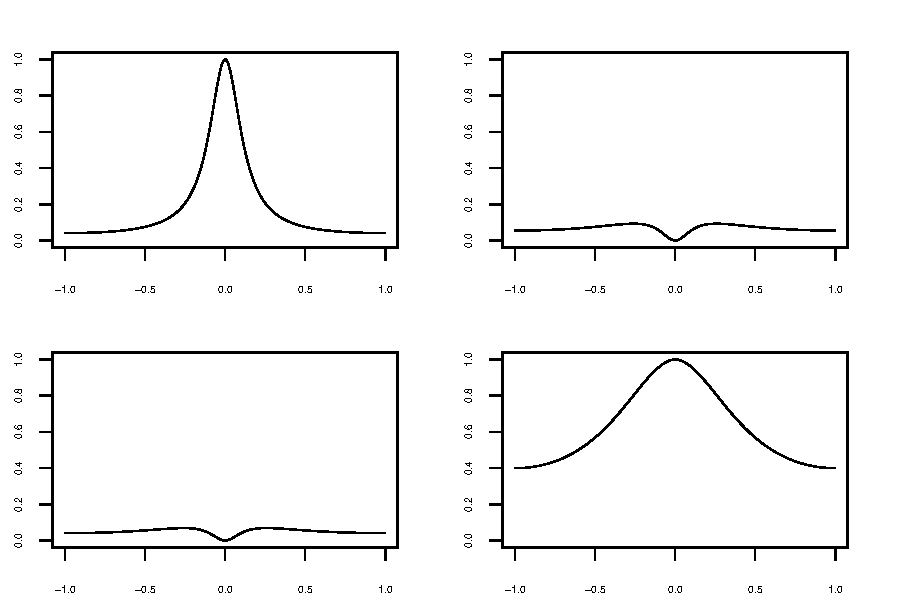
\includegraphics[]{llm_frf.pdf}
\caption{Frequency response function for model-based trend
 extraction filter from the Local Level Model.}
\label{fig:llm-frf}
\end{center}
\end{figure} 


\begin{Example} {\bf Model-Based Integrated Random Walk Trend.} \rm
\label{exam:trend-i2}
  Example \ref{exam:trend-i1} can be generalized to the Smooth 
  Trend Model (STM) developed in Harvey (1989),
 where now the trend $\{ S_t \}$ is an integrated random walk, 
 i.e., ${(1-L)}^2 S_t$ is white noise of
 covariance matrix $\Sigma_{S}$.   Then the frf for the optimal 
 trend extraction filter -- which also coincides
 with the multivariate HP filter  -- is given by
\[ 
 \Psi (e^{-i \omega}) = e_j^{\prime} \, \Sigma_{S} \, 
 { \left[ \Sigma_{S} + {(2 - 2 \, \cos (\omega))}^2 \, \Sigma_{N} \right] }^{-1}.
\]
 The chief difference with the frf of the LLM is that the sinusoidal factor is now squared.  
\end{Example}

\begin{Exercise} {\bf STM Model-Based Trend Filter.} \rm
\label{exer:trend-i2}
 For a bivariate STM of Example \ref{exer:trend-i2} with parameters 
\[
 \Sigma_{S} = 10^{-5} \, \left[ \begin{array}{ll} 
   .66   &  1.25   \\
   1.25  &  2.92   \end{array}  \right]
 \qquad  \Sigma_{N} =  10^{-4} \, \left[ \begin{array}{ll}
        2.52  &  1.67    \\
        1.67 &  35.70   \end{array} \right],
\]
 numerically compute and plot the trend extraction filter's frf.
\end{Exercise}


\begin{Schunk}
\begin{Sinput}
> psi.sim <- c(1.8905590615422, -11.9288577633298, -12.0809347541079, 
+              0.660897814610799, -8.2863379601304, -5.66645335346871, 
+              -1.34743227511595e-05, -1.41207967213544e-05)
> psi.sim[7:8] <- c(0,0)
> N <- 2
> grid <- 1000
> delta <- array(t(c(1,-2,1)) %x% diag(N),c(N,N,3))
> mu.sim <- mdfa.wnsim(psi.sim[1:3],rep(1,N),10,Inf)
> Sigma.mu <- mu.sim[[2]]
> irr.sim <- mdfa.wnsim(psi.sim[4:6],rep(1,N),10,Inf)
> Sigma.irr <- irr.sim[[2]]
> #print(Sigma.mu)
> #print(Sigma.irr)
> 
> iden <- array(diag(N),c(N,N,1))
> f.mu <- mdfa.spectra(iden,iden,Sigma.mu,grid)
> f.irr <- mdfa.spectra(iden,iden,Sigma.irr,grid)
> trend.frf <- mdfa.wkfrf(iden,delta,f.irr,f.mu)
\end{Sinput}
\end{Schunk}


 \begin{figure}[htb!]
\begin{center}
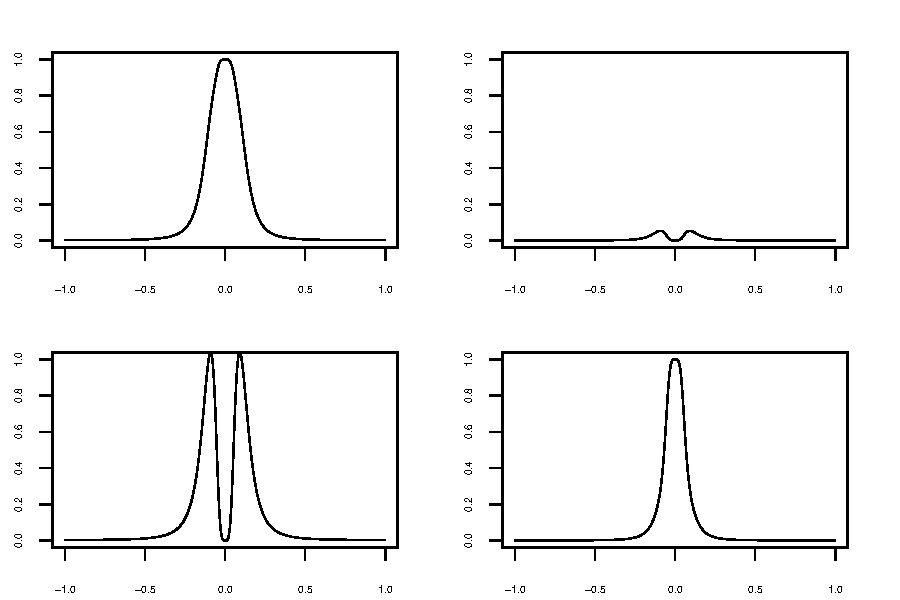
\includegraphics[]{stm_frf.pdf}
\caption{Frequency response function for model-based trend
 extraction filter from the Smooth Trend Model.}
\label{fig:stm-frf}
\end{center}
\end{figure} 


\begin{Example} {\bf Model-Based Seasonal Adjustment.} \rm
\label{exam:sa}
  Flexible structural models were discussed in McElroy (2017), 
  with atomic components for each distinct unit root
 (with any conjugate roots) in the differencing operator.  
 For monthly data  where $\delta (L) = (1-L)(1-L^{12})$,
 we obtain an integrated random walk trend component $\{ C_t \}$ 
 (identical to the trend discussed in Example \ref{exam:trend-i2})
 and six atomic seasonal components that combine into a single 
 seasonal component $\{ P_t \}$ with differencing
 operator $U(L) = 1 + L + L^2 + \ldots + L^{11}$, along with the
 irregular $\{ I_t \}$, which is a white noise. 
  Six separate covariance matrices govern the dynamics of the seasonal
  component, allowing for different degrees of
 smoothness at each of the six seasonal frequencies. 
 In particular, we have $P_t = \sum_{\ell=1}^6 P^{(\ell)}_t$ and
\begin{align*}
  {(1-L)}^2 C_t & = \partial C_t \\
   (1 - 2 \cos (\pi/6) L + L^2) P^{(1)}_t & = \partial P^{(1)}_t \\
  (1 - 2 \cos (2\pi/6) L + L^2) P^{(2)}_t & = \partial P^{(2)}_t \\
  (1 - 2 \cos (3\pi/6) L + L^2) P^{(3)}_t & = \partial P^{(3)}_t \\
  (1 - 2 \cos (4\pi/6) L + L^2) P^{(4)}_t & = \partial P^{(4)}_t \\
  (1 - 2 \cos (5\pi/6) L + L^2) P^{(5)}_t & = \partial P^{(5)}_t \\
  (1 +L) P^{(6)}_t & = \partial P^{(6)}_t. 
 \end{align*}
 Each of the stationary processes is assumed to be an independent white noise,
 where the covariance matrices are denoted by $\Sigma_C$, $\Sigma_{1}$,
  $\Sigma_2$, $\Sigma_3$, $\Sigma_4$, $\Sigma_5$, $\Sigma_6$, and 
  $\Sigma_I$ respectively.   For seasonal adjustment we seek to suppress
  seasonality, so $S_t = C_t + I_t$ and $N_t = P_t$.  Thus $\delta^S (z) = {(1-z)}^2$
  and $\delta^N (z) = U(z)$, and the MB seasonal adjustment filter   has frf
\[
  \Psi (e^{-i \omega}) = e_j^{\prime} \, \left( \Sigma_{C} + {|1 - e^{-i \omega}|}^4
   \Sigma_I \right) \, 
    { f_{\partial X} (\omega) }^{-1} \, {| U (e^{-i \omega}) |}^2.
\]
\end{Example}


\begin{Exercise} {\bf Structural Model-Based Seasonal Adjustment.} \rm
\label{exer:sa}
 Consider a quadvariate structural model of Example \ref{exer:sa} with parameters 
\begin{align*}
 \Sigma_C & = 10^{-2} \, \left[ \begin{array}{llll} 
  9.54 & 4.71 & 1.70 &  3.26  \\
  4.71 & 2.74 & 1.01 & 1.96  \\
  1.70 & 1.01 & 0.49 & 0.81 \\
  3.26 & 1.96 & 0.81 &  1.70  \end{array} \right] \\
  \Sigma_1 & = 10^{-2} \, \left[ \begin{array}{llll} 
 7.97 & 6.98 & 1.77 & 3.99 \\
 6.98 & 7.47 & 2.01 & 4.57 \\
 1.77 & 2.01 & 0.80 & 1.50 \\
 3.99 & 4.57 & 1.50 & 3.85 \end{array} \right] \\
   \Sigma_2 & = 10^{-2} \, \left[ \begin{array}{llll} 
 1.76 & 0.17 & 0.35 & 1.49 \\
 0.17 & 0.94 & 0.48 & 0.72 \\
 0.35 & 0.48 & 1.17 & 1.58 \\
 1.49 & 0.72 & 1.58 & 4.49 \end{array} \right] \\
    \Sigma_3 & = 10^{-2} \, \left[ \begin{array}{llll} 
  4.71 &  4.35 & -1.87 &  1.15 \\
  4.35 &  4.89 & -2.04 &  1.38 \\
 -1.87 & -2.04 &  1.55 & -0.04 \\
  1.15 &  1.38 & -0.04 &  1.43 \end{array} \right] \\
    \Sigma_4 & = 10^{-2} \, \left[ \begin{array}{llll} 
 12.56 &  3.30 & -2.28  & 1.88 \\
  3.30 &  3.49 & -0.88 &  1.06 \\
 -2.28 & -0.88 &  0.78 & -0.45 \\
  1.88 &  1.06 & -0.45 &  0.88 \end{array} \right] \\
     \Sigma_5 & = 10^{-2} \, \left[ \begin{array}{llll} 
 1.07 & 1.51 & -0.01 & -0.24  \\
 1.51 & 3.04 &  0.01  & 0.79 \\
-0.01 & 0.01  & 0.09  & 0.05 \\
-0.24 & 0.79  & 0.05  & 1.69 \end{array} \right] \\
     \Sigma_6 & = 10^{-2} \, \left[ \begin{array}{llll} 
 11.79 & -1.17 &   1.38 &  1.86 \\
 -1.17 &   2.77 & -0.23 & 0.30 \\
  1.38 & -0.23 &   0.77 & 0.40 \\
  1.86  & 0.30  & 0.40 & 3.11 \end{array} \right] \\
      \Sigma_I & =  \left[ \begin{array}{llll} 
  6.53 & 0.81 & 0.19 & -0.57 \\
  0.81 & 1.26 & 0.23  & 0.49 \\
  0.19 & 0.23 & 0.30  & 0.15 \\
 -0.57 & 0.49 & 0.15  & 1.08 \end{array} \right].
\end{align*} 
 Numerically compute and plot the  filter frf for seasonal adjustment.
\end{Exercise}

\begin{Schunk}
\begin{Sinput}
> psi.sim <- c(0.493586093056948, 0.178487258592539, 0.341217399125708, 
+              0.399177274154249, 0.848325304642642, 0.68306879252262, 
+              -2.3494687111314, -5.47534663726587, -6.69385117951384, 
+              -6.08364145983965, 0.875100150810273, 0.221971271148611, 
+              0.500866759201029, 0.340625016984097, 0.791037805495801, 
+              0.985440262768576, -2.52890913740106, -4.29524634814519, 
+              -5.98519527750281, -4.88659954275053, 0.0957466327314851, 
+              0.201313350626488, 0.849351809157598, 0.48420520104336, 
+              0.62643997675928, 1.13945063379914, -4.04217214895869, 
+              -4.68919816059416, -4.73313805629826, -4.0627015759002,
+              0.923495751608401, -0.396067294450726, 0.244665046194039, 
+              -0.36570474542918, 0.363995718736632, 0.758715172737758, 
+              -3.05567431351817, -4.74337970092605, -4.96364133429136, 
+              -5.06144086942249, 0.262963683605793, -0.181599400661918, 
+              0.149795833258992, -0.105991649100357, 0.21503766242974, 
+              -0.141649861043968, -2.07489346121933, -3.64302004053168, 
+              -5.69277788172285, -5.3689470753418, 1.40718934367933,
+              -0.0085452878747676, -0.219886337273936, 0.0283662345070971,
+              1.23786259577472, 0.199834135215749, -4.53336362894347, 
+              -4.70016052568401, -7.07530853221777, -6.03054443735399, 
+              -0.0995506040524902, 0.116607848697947, 0.157899802233636, 
+              -0.0363184981547607, 0.18385749297074, 0.329351477585333, 
+              -2.1377604820296, -3.62882764786239, -5.11279846492415, 
+              -3.62475631527416, 0.124305286145147, 0.0292507920421885, 
+              -0.0873349194845382, 0.178977764316143, 0.484389128732254,
+              0.265835976421986, 1.87566939226944, 0.1445002084775, 
+              -1.34264222816582, -0.305367634014929, -0.00488431480035087, 
+              -0.000945659564684563, -0.00106126820173145, -0.000413658838890233)
> psi.sim[81:84] <- c(0,0,0,0)
> N <- 4
> grid <- 1000
> mu.sim <- mdfa.wnsim(psi.sim[1:10],rep(1,N),10,Inf)
> Sigma.mu <- mu.sim[[2]]
> seas1.sim <- mdfa.wnsim(psi.sim[11:20],rep(1,N),10,Inf)
> Sigma.seas1 <- seas1.sim[[2]]
> seas2.sim <- mdfa.wnsim(psi.sim[21:30],rep(1,N),10,Inf)
> Sigma.seas2 <- seas2.sim[[2]]
> seas3.sim <- mdfa.wnsim(psi.sim[31:40],rep(1,N),10,Inf)
> Sigma.seas3 <- seas3.sim[[2]]
> seas4.sim <- mdfa.wnsim(psi.sim[41:50],rep(1,N),10,Inf)
> Sigma.seas4 <- seas4.sim[[2]]
> seas5.sim <- mdfa.wnsim(psi.sim[51:60],rep(1,N),10,Inf)
> Sigma.seas5 <- seas5.sim[[2]]
> seas6.sim <- mdfa.wnsim(psi.sim[61:70],rep(1,N),10,Inf)
> Sigma.seas6 <- seas6.sim[[2]]
> irr.sim <- mdfa.wnsim(psi.sim[71:80],rep(1,N),10,Inf)
> Sigma.irr <- irr.sim[[2]]
> #print(Sigma.mu)
> #print(Sigma.seas1)
> #print(Sigma.seas2)
> #print(Sigma.seas3)
> #print(Sigma.seas4)
> #print(Sigma.seas5)
> #print(Sigma.seas6)
> #print(Sigma.irr)
> 
> iden <- array(diag(N),c(N,N,1))
> dpoly.1 <- c(1,-2*cos(pi/6),1)
> dpoly.2 <- c(1,-2*cos(2*pi/6),1)
> dpoly.3 <- c(1,-2*cos(3*pi/6),1)
> dpoly.4 <- c(1,-2*cos(4*pi/6),1)
> dpoly.5 <- c(1,-2*cos(5*pi/6),1)
> dpoly.6 <- c(1,1)
> dpoly.but1 <- polymult(dpoly.2,polymult(dpoly.3,polymult(dpoly.4,polymult(dpoly.5,dpoly.6))))
> dpoly.but2 <- polymult(dpoly.1,polymult(dpoly.3,polymult(dpoly.4,polymult(dpoly.5,dpoly.6))))
> dpoly.but3 <- polymult(dpoly.1,polymult(dpoly.2,polymult(dpoly.4,polymult(dpoly.5,dpoly.6))))
> dpoly.but4 <- polymult(dpoly.1,polymult(dpoly.2,polymult(dpoly.3,polymult(dpoly.5,dpoly.6))))
> dpoly.but5 <- polymult(dpoly.1,polymult(dpoly.2,polymult(dpoly.3,polymult(dpoly.4,dpoly.6))))
> dpoly.but6 <- polymult(dpoly.1,polymult(dpoly.2,polymult(dpoly.3,polymult(dpoly.4,dpoly.5))))
> delta.c <- array(t(c(1,-2,1)) %x% diag(N),c(N,N,3))
> delta.but1 <- array(t(dpoly.but1) %x% diag(N),c(N,N,10))
> delta.but2 <- array(t(dpoly.but2) %x% diag(N),c(N,N,10))
> delta.but3 <- array(t(dpoly.but3) %x% diag(N),c(N,N,10))
> delta.but4 <- array(t(dpoly.but4) %x% diag(N),c(N,N,10))
> delta.but5 <- array(t(dpoly.but5) %x% diag(N),c(N,N,10))
> delta.but6 <- array(t(dpoly.but6) %x% diag(N),c(N,N,11))
> delta.seas <- array(t(rep(1,12)) %x% diag(N),c(N,N,12))
> f.mu <- mdfa.spectra(iden,iden,Sigma.mu,grid)
> f.seas1 <- mdfa.spectra(iden,delta.but1,Sigma.seas1,grid)
> f.seas2 <- mdfa.spectra(iden,delta.but2,Sigma.seas2,grid)
> f.seas3 <- mdfa.spectra(iden,delta.but3,Sigma.seas3,grid)
> f.seas4 <- mdfa.spectra(iden,delta.but4,Sigma.seas4,grid)
> f.seas5 <- mdfa.spectra(iden,delta.but5,Sigma.seas5,grid)
> f.seas6 <- mdfa.spectra(iden,delta.but6,Sigma.seas6,grid)
> f.irr <- mdfa.spectra(iden,delta.c,Sigma.irr,grid)
> f.signal <- f.mu + f.irr
> f.noise <- f.seas1 + f.seas2 + f.seas3 + f.seas4 + f.seas5 + f.seas6
> sa.frf <- mdfa.wkfrf(delta.seas,delta.c,f.noise,f.signal)
\end{Sinput}
\end{Schunk}


\begin{figure}[htb!]
\begin{center}
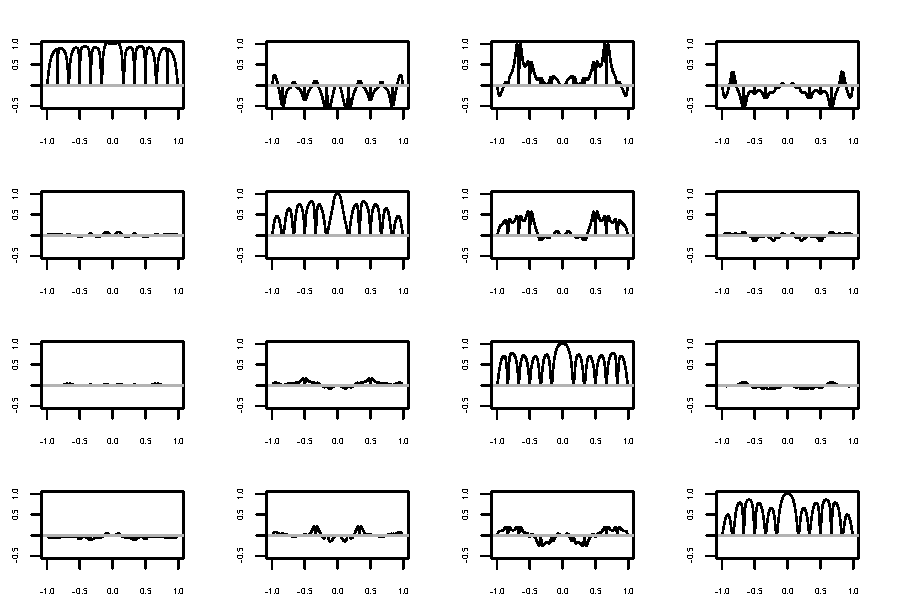
\includegraphics[]{sauc_frf.pdf}
\caption{Frequency response function for model-based seasonal adjustment
  filter from the Structural Model.}
\label{fig:sauc-frf}
\end{center}
\end{figure} 



\section{Error Criterion and Computation}
\label{sec:mdfa-nonstat}

We now consider LPPs for non-stationary processes. 
 The definition of target is the same as that given in Definition \ref{def:target2},
 and the LPP is still defined via Definition \ref{def:lpp2},
 but now the underlying process is non-stationary.  This changes
  slightly the solution, because forecasting must take the non-stationarity
  into account.
 

\begin{Proposition}
 \label{prop:GPP-nonstat}
 Suppose that $\{ X_t \}$ is  a non-stationary stochastic process
 with representation (\ref{eq:nonstatCausalRep}), such that
 $\{ \partial X_t \}$ is mean zero and weakly stationary 
 with  causal Wold decomposition expressed as $\partial X_t = \Theta (L) \, \epsilon_t$,
 where $\Theta (L)$ is invertible and
  $\{ \epsilon_t \}$ is white noise of covariance $\Sigma$.
  Then the solution
 to the LPP posed by a   target $Y_t = \Psi (L) \, X_t$ is given by
\begin{equation}
 \label{eq:GPPsoln-nonstat}
  \widehat{\Psi} (L) = \sum_{\ell = 0}^{\infty} \psi (\ell) \, L^{\ell}
    + \sum_{ \ell = -1}^{- \infty} \psi (\ell) \, 
\left(  \sum_{h=0 }^{d-1} A_{-\ell} (h) L^{h} + \sum_{k=1}^{-\ell} \xi_{-\ell-k}
  { [  \Theta (L) ] }_{k}^{\infty} L^{-k} \delta (L) { \Theta (L)}^{-1} 
 \right).
\end{equation}
 Moreover, the   MSE  corresponding to this solution is given by
\begin{equation} 
\label{eq:minimalMSE}
 \frac{1}{ 2 \pi} \int_{-\pi}^{\pi}   \sum_{\ell, k > 0 } \psi (-\ell) \,
  {[ \Theta  (e^{-i \omega}) / \delta (e^{-i \omega}) ]}_0^{\ell-1}   \,  \Sigma \,
  { {[ \Theta  (e^{i \omega}) / \delta (e^{i \omega}) ]}_0^{ k-1} }^{\prime}  \,
   {\psi (-k) }^{\prime} \,  e^{i \omega (\ell - k) }   \, d\omega.
\end{equation}
 \end{Proposition}
 
\paragraph{Proof of Proposition \ref{prop:GPP-nonstat}.} 
 We show that the filter error $\Delta (z) = \Psi (z) - \widehat{\Psi} (z)$
  is divisible by $\delta (z)$, so that we can write
   $\Delta (z) = \widetilde{\Delta} (z) \delta (z)$, from which it follows
    that the error process must be stationary.
  We make use of an algebraic identity proved in McElroy and Findley (2010):
  for any $j \geq 0$
\begin{equation}
 \label{eq:diffop-algid}
  {[ \Theta (z)/ \delta (z)]}_0^{j} = \sum_{k=0}^j \xi_k z^k { [ \Theta (z) ] }_0^{j-k}.
\end{equation}
 Then using the definition of $\widehat{\Psi}(L)$ in (\ref{eq:GPPsoln-nonstat}),
\begin{align*}    
  \Delta (z) & =  \sum_{\ell = -1}^{- \infty} \psi (\ell) 
   \left( z^{\ell} - \sum_{h=0}^{d-1} A_{-\ell} (h) z^h  - \sum_{k=1}^{-\ell} \xi_{-\ell-k}
    {[ \Theta (z)]}_k^{\infty} z^{-k} \delta (z) { \Theta (z)}^{-1}  \right) \\
    & = \sum_{\ell = -1}^{- \infty} \psi (\ell) 
   \left( \sum_{k=0}^{-\ell-1} \xi_k z^{k+\ell} \Theta (z) -
     \sum_{k=0}^{-\ell-1} \xi_{k}
    {[ \Theta (z)]}_{-\ell-k}^{\infty} z^{k+\ell} \delta (z) { \Theta (z)}^{-1} \right) \\
  & = \sum_{\ell = -1}^{- \infty} \psi (\ell) 
   \left( \sum_{k=0}^{-\ell-1} \xi_k z^{k+\ell} 
    {[ \Theta (z)]}_0^{-\ell-k-1}   \right) \delta (z) { \Theta (z)}^{-1} \\
   & = \sum_{\ell = -1}^{- \infty} \psi (\ell) z^{\ell}
    { [ \Theta (z) / \delta (z)]}_0^{-\ell-1} 
    \delta (z) { \Theta (z)}^{-1},
\end{align*}    
   where the second equality follows from (\ref{eq:Identity1}), 
    and the fourth equality  follows from (\ref{eq:diffop-algid}).
    Hence, we find that
\[
 \widetilde{\Delta} (z) = \sum_{\ell = -1}^{- \infty} \psi (\ell) z^{\ell}
    { [ \Theta (z) / \delta (z)]}_0^{-\ell-1}  { \Theta (z)}^{-1},
\]
 which is well-defined under the invertibility assumption.  
 The real-time error process is then
\[
  \Delta (L) X_t = \widetilde{\Delta} (L) \, \partial X_t
    = \sum_{\ell = -1}^{- \infty} \psi (\ell)  
    { [ \Theta (L) / \delta (L)]}_0^{-\ell-1}\, \epsilon_{t-\ell},
\]
 which only involves future innovations.  Hence the error process is 
  uncorrelated with present and past values of the process $\{ X_t \}$,
   demonstrating optimality.  The MSE is computed 
 by taking the variance of the error process.  $\qquad \Box$

% \widehat{\Psi} (L) = \sum_{\ell = -\infty }^{\infty} \psi (\ell) \, L^{\ell} - 
% \sum_{\ell < 0 } \psi (\ell)
% \,  { [ \Theta (L) / \delta (L) ]}_{0}^{ -\ell-1  } \, L^{\ell} \,
% {\Theta (L) }^{-1} \delta(L).

 
\vspace{.5cm}

 Proposition  \ref{prop:GPP-nonstat} gives the optimal concurrent filter in 
  the non-stationary case, and the answer depends upon knowing the process'
   dynamics.  However, for MDFA we wish to proceed without such an assumed
   knowledge.   From the proof of Proposition  \ref{prop:GPP-nonstat}, it
  is clear that  the error process will  
 not be stationary unless we make certain assumptions
 about $\Delta (L) = \Psi (L) - \widehat{\Psi} (L)$.    
 In order to remove the time-varying functions it is necessary that 
 we can factor $\delta (L)$ from $\Delta (L)$, i.e., we require the existence of
 $\widetilde{\Delta } (L)$ such that
\begin{equation}
 \label{eq:delta.factor}
  \Delta (L) = \widetilde{\Delta } (L) \, \delta (L),
\end{equation}
 as otherwise we cannot guarantee that $\{ E_t \}$ will be stationary. 
 (This condition (\ref{eq:delta.factor}) is indeed satisfied by the optimal 
 concurrent filter of Proposition \ref{prop:GPP-nonstat}, as is shown in the 
  proof.)  Moreover, if $\mu =0$ then (\ref{eq:delta.factor}) is also 
  sufficient to guarantee
 that the filter error be stationary, because
\[
  E_t = \widetilde{\Delta} (L) \, \partial X_t
\]
 in such a case.   We next discuss a set of filter 
 constraints that guarantee (\ref{eq:delta.factor}), beginning with a result
 that discusses the factorization of filters.  
 We say a filter $\Psi (L)$ is absolutely convergent 
 if $\sum_{j \in \ZZ} \| \psi (j) \| < \infty$
 for a given matrix norm $\| \cdot \|$.

\begin{Proposition}
\label{prop:filter-decompose}
 Any linear filter $\Psi (L)$ can be expressed as
\[
  \Psi (L) = \Psi (\zeta) + (L - \zeta) \, \Psi^{\sharp} (L)
\]
 for any $\zeta \in \CC$  such that $| \zeta | = 1$,
  and an absolutely convergent filter $\Psi^{\sharp} (L)$,
  so long as  $\partial \Psi (L) $ is absolutely convergent.
 If in addition $ \partial \partial \Psi (L) =
 \sum_{ j \in \ZZ} j (j-1) \, \psi (j) \, L^j$
   is absolutely convergent, then there also exists an absolutely
   convergent filter $\Psi^{\flat} (L)$  such that
\[
 \Psi (L) = \Psi (\zeta) + \partial \Psi (\zeta) \, 
 (L- \zeta) \, \overline{\zeta} + {(L - \zeta)}^2 \, \Psi^{\flat} (L).
\]
\end{Proposition}


\paragraph{Proof of Proposition \ref{prop:filter-decompose}.}
 We claim that $\Psi^{\sharp} (L) = \sum_{j \in \ZZ} \psi^{\sharp} (j) \, L^j$ with
\[
 \psi^{\sharp} (j) = \begin{cases}  {\zeta}^{-(j+1)} \,  
 \sum_{k \geq j+1} \psi (k) \, \zeta^k  \quad j \geq 0 \\
					-\zeta^{-(j+1)} \, \sum_{k \geq -j} \psi (-k) \,  
					{\zeta}^{-k} \quad j \leq -1.	
		\end{cases}
\]
To show this, first observe that 
\[
  \Psi (L) - \Psi (\zeta) = \sum_{j \geq 1} \psi (j) \, 
  (L^j - \zeta^j) + \sum_{j \leq -1} \psi (j) \, (L^j - \zeta^j).
\]
 Beginning with the first term, so that $j \geq 1$, we write 
 $L^j - \zeta^j = \zeta^j \, (L/\zeta - 1) \, p_{j-1} (L/\zeta)$
 where $p_k (z) = \sum_{\ell=0}^k z^{\ell}$.   Next, by coefficient
 matching we can verify that
\begin{align*}
   \sum_{j \geq 1} \psi (j) \, (L^j - \zeta^j) & = (L/\zeta - 1) \,
   \sum_{j \geq 1} \psi (j) \, \zeta^j \, p_{j-1} (L/\zeta) \\
 & = (L/\zeta -1) \, \sum_{j \geq 0}  \sum_{k \geq j+1} \psi (k) \,
 \zeta^k \, {(L/\zeta)}^{j}
 = (L - \zeta) \,  \sum_{j \geq 0}  \psi^{\sharp} (j) \, L^j.
\end{align*}
 Next, take $j \leq -1$, and use the symbol $F = L^{-1}$:
\begin{align*}
  \sum_{j \leq -1} \psi (j) \, (L^j - \zeta^j) & = \sum_{j \geq 1}
  \psi (-j) \, (F^j - \zeta^{-j}) 
   =   (F \zeta - 1) \, \sum_{j \geq 1} \psi (-j) \, \zeta^{-j} \, p_{j-1} (F \zeta) \\
 & =  (F \zeta - 1) \, \sum_{j \geq 0} \sum_{k \geq j+1}  
  \psi (-k) \, \zeta^{-k} \, {(F \zeta)}^{j}  \\
 &  =  - F\,  (L - \zeta ) \, \sum_{j \geq 1}  \zeta^{j-1} 
 \, \sum_{k \geq j}  \psi (-k) \, \zeta^{-k} \,  F^{j-1}  \\
 &= (L - \zeta) \, \sum_{j \leq -1}  \psi^{\sharp} (j) \, L^j.
\end{align*}
 This establishes algebraically that $\Psi^{\sharp} (L)$ 
 with coefficients as defined above equals
 $(\Psi (L) - \Psi (\zeta))/(L- \zeta)$, whenever the Laurent
 series converges.  Based on the above calculations, we can write
\[
  \frac{ \Psi (L) - \Psi (\zeta) }{ L - \zeta} 
  = \sum_{j \geq 1} \left( \psi (j) \, \zeta^{j-1} \, p_{j-1}
  (L/\zeta) - \psi (-j) \, \zeta^{-j} \, F \, p_{j-1} (F \zeta) \right).
\]
 To check the absolute convergence, it suffices to set $L = 1$;  
 note that $| p_k  (\zeta) | \leq (k+1)$
 if $|\zeta| = 1$.  Thus  we obtain the bound
\[
 \left\|   \frac{ \Psi (L) - \Psi (\zeta) }{ L - \zeta}  \right\| 
 \leq \sum_{j \geq 1}  j \, \left( \| \psi (j) \|  +\| \psi (-j) \| \right),
\]
 which is finite by the assumption that $\partial \Psi (L)$ 
 is absolutely convergent.   Next, we claim that
$\Psi^{\flat} (L) = \sum_{j \in \ZZ} \psi^{\flat} (j) \, L^j$ with
\[
 \psi^{\flat} (j) = \begin{cases}  {\zeta}^{-(j+2)} \, 
 \sum_{k \geq j+2} (k-1-j) \, \psi (k) \, \zeta^k  \quad j \geq 0 \\
					\zeta^{-(j+2)} \, \sum_{k \geq -j} (k+j+1) \,
					\psi (-k) \,  {\zeta}^{-k} \quad j \leq -1.	
		\end{cases}
\]
To verify this, observe that
\begin{align*}
  \Psi (L) - \Psi (\zeta)  - \partial \Psi (\zeta) \, (L- \zeta) \, \zeta^{-1} 
 & = \sum_{j \geq 1} \psi (j) \, \left[ (L^j - \zeta^j)  
 - j \, \zeta^{j-1}   \, (L- \zeta) \right]  \\
& + \sum_{j \leq -1} \psi (j) \, \left[ (L^j - \zeta^j)  
- j \, \zeta^{j-1}   \, (L- \zeta) \right].
\end{align*}
 First assuming that $j \geq 1$, note that $p_{\ell-1} (z) - \ell$
 equals zero unless $\ell \geq 2$, 
 and otherwise   equals $\sum_{k=1}^{\ell-1} p_{k-1} (z) \, (z -1)$. Therefore 
\begin{align*}
 \sum_{j \geq 1} \psi (j) \, \left[ (L^j - \zeta^j)  
 - j \, \zeta^{j-1}  \, (L- \zeta) \right]    & 
 = (L- \zeta) \, \sum_{j \geq 1} \psi (j) \, 
 \zeta^{j-1} \, \left[   p_{j-1} (L/\zeta) 	  - j   \right]   \\
 & =  {(L - \zeta)}^2 \, \sum_{j \geq 2} \psi (j) \, 
 \zeta^{j-2} \, \sum_{k=1}^{j-1} p_{k-1} (L/\zeta)   \\
 & =  {(L - \zeta)}^2 \, \sum_{j \geq 0} \psi^{\flat} (j) \,  L^j 
\end{align*}
 by coefficient matching in the final step.  Similarly, letting $j \leq -1$ 
 and using $z p_{\ell-1} (z) - \ell = (z-1) \, 
 \sum_{k=1}^{\ell} p_{k-1} (z)$, we have
\begin{align*}
 \sum_{j \leq -1} \psi (j) \, \left[ (L^j - \zeta^j) 
 - j \, \zeta^{j-1}  \, (L- \zeta) \right]    & 
  =  (L- \zeta) \, \sum_{j \geq 1} \psi (-j) \, \zeta^{-j} \,
  \left[ - F \,  p_{j-1} (F \zeta)  +  j  \, \zeta^{-1} \right]   \\
 & =  {(L- \zeta)}^2 \, F \, \sum_{j \geq 1} \psi(-j) \, 
 \zeta^{-(j+1)} \, \sum_{k=1}^{j} p_{k-1} (F \zeta)  \\
 & = {(L- \zeta)}^2 \, F \, \zeta^{-1} \, \sum_{j \geq 0} 
 \sum_{k \geq j+1}  (k-j) \, \psi (-k) \, \zeta^{-k} \, {(F \zeta)}^j \\
 & = {(L-\zeta)}^2 \,  \sum_{j \leq -1}  \psi^{\flat} (j) \, L^j
\end{align*}
 by matching coefficients.  To establish convergence of the 
 Laurent series for $\Psi^{\flat} (L)$,  observe that
\[
 \frac{  \Psi (L) - \Psi (\zeta)  - \partial \Psi (\zeta) 
 \, (L- \zeta) \, \zeta^{-1}  }{ {(L- \zeta)}^2 } =
    \sum_{j \geq 2} \psi (j) \, \zeta^{j-2} \, \sum_{k=1}^{j-1} p_{k-1} (L/\zeta) +
     F \, \sum_{j \geq 1} \psi(-j) \, \zeta^{-(j+1)} \, \sum_{k=1}^{j} p_{k-1} (F \zeta).
\]
 Hence the matrix norm has   the bound (setting $L=1$ and taking $|\zeta| = 1$) of
\[
 \left\|   \frac{  \Psi (L) - \Psi (\zeta) 
 - \partial \Psi (\zeta) \, (L- \zeta) \, \zeta^{-1}  }{ {(L- \zeta)}^2 }  \right\|
  \leq  \sum_{j \geq 2} \| \psi (j)  \|  \, \binom{j}{2} + 
  \sum_{j \geq 1} \| \psi(-j)  \|  \, \binom{j+1}{2},
\]
 using $| \sum_{k=1}^j p_{k-1} (\zeta) | \leq \binom{j+1}{2}$.  
 Because $\partial \partial \Psi (L)$ is 
 absolutely convergent, the above norm is finite.  $\quad \Box$

\vspace{.5cm}

 Note that if $\Psi (\zeta) = 0$, it follows from 
  Proposition \ref{prop:filter-decompose} that $L-\zeta$ can be factored from
  $\Psi (L)$.  Similarly, ${(L- \zeta)}^2$ can be factored 
   from $\Psi (L)$ if $\Psi(\zeta) = \partial \Psi (\zeta) =0$.
  Next, we introduce the concept of $\omega$-dynamics, which correspond
  to basis functions $\phi_k (t) = e^{i \omega t}$.

\begin{Definition} \rm
\label{def:filter-noise}
 For $\omega \in [-\pi, \pi]$, a filter $\Psi (L)$ annihilates 
 $\omega$-dynamics of order $1$ if $\Psi (e^{-i \omega}) = 0$,
 and annihilates $\omega$-dynamics of order $2$ if in addition 
 $\partial \Psi (e^{-i \omega}) = 0$.
\end{Definition}


Hence, we have the following immediate corollary of 
Proposition \ref{prop:filter-decompose}.

\begin{Corollary}
 \label{cor:filter-noise}
  If a filter $\Psi (L)$ annihilates $\omega$-dynamics of order $1$ 
  and $\partial \Psi (L)$ is absolutely convergent, then
\[
  \Psi (L) = (L- e^{-i \omega}) \, \Psi^{\sharp} (L).
\]
 If a filter $\Psi (L)$ annihilate $\omega$-dynamics of order $2$,  
 and $\partial \partial \Psi (L)$ is absolutely convergent, then
\[
  \Psi (L) = {(L- e^{-i \omega}) }^2 \, \Psi^{\flat} (L).
\]
\end{Corollary}

 We can apply Corollary \ref{cor:filter-noise} to factor a 
 noise-differencing polynomial $\delta^N (L)$ from $\Delta (L)$:
 for each $\omega$ such that the target filter $\Psi (L)$ annihilates
 $\omega$-dynamics of order $d$, we impose the constraint
 that $\widehat{\Psi} (L)$ shall have the same property, and hence 
 ${(L- e^{-i \omega})}^d$ can be factored from both
 filters.   For instance, if noise frequencies are $\omega_{\ell}$
 with multiplicities $d_{\ell}$, then repeated application of
 Corollary \ref{cor:filter-noise} yields
\[
 \Psi (L) = \prod_{\ell} {(L -  e^{-i \omega_{\ell}})}^{d_{\ell}} \, \Psi^{\natural} (L)
   = \delta^N (L) \, \Psi^{\star} (L)
\]
 for some residual filter $\Psi^{\natural} (L)$, where 
 $\Psi^{\star} (L) = \prod_{\ell} (-e^{-i \omega_{\ell} d_{\ell}}) \, \Psi^{\natural} (L)$
 and $\delta^N (L) = \prod_{\ell} (1 - e^{i \omega_{\ell}} \, L)$.
 By imposing the same linear constraints on $\widehat{\Psi} (L)$, 
 we likewise obtain $\widehat{\Psi} (L) = \delta^N (L) \, \widehat{\Psi}^{\star} (L)$,
 and hence
\begin{equation}
 \label{eq:delta-noise}
\Delta (L) = \left(  {\Psi}^{\star} (L) - 
\widehat{\Psi}^{\star} (L) \right) \, \delta^N (L).
\end{equation}
  So if $\delta (L) = \delta^N (L)$, then (\ref{eq:delta.factor}) 
  holds at once.  More generally, a given process' differencing polynomial
 may be factored into relatively prime polynomials $\delta^N (z)$ and $\delta^S (z)$, 
 which correspond to noise and signal dynamics
 respectively -- see Bell (1984) and McElroy (2008a). 
 Many  signal extraction filters $\Psi (L)$   have the property that they
 annihilate $\omega$-dynamics of the appropriate order, 
 such that $\delta^N (L)$ can be factored.
 By imposing that 
\begin{equation}
\label{eq:non-stat.constraint.single}
 \widehat{\Psi} (e^{-i \omega}) = \Psi (e^{-i \omega})
 \end{equation}
 for  all simple roots $\zeta = e^{-i \omega}$ of $\delta (z)$, we ensure that
  (\ref{eq:delta.factor}) holds. If there is a double root, then we also impose
 \begin{equation}
\label{eq:non-stat.constraint.double}
 \partial \widehat{\Psi} (e^{-i \omega}) = \partial \Psi (e^{-i \omega}).
 \end{equation}
   These conditions are sufficient, because 
  (\ref{eq:non-stat.constraint.single}) and  (\ref{eq:non-stat.constraint.double})
    imply $\Delta (e^{-i \omega}) = 0$
  for all the roots of $\delta (z)$, so that by repeated application of Corollary 
 \ref{cor:filter-noise} we can factor out $\delta (z)$, labelling the
 remaining factor as $\widetilde{\Delta } (L)$.  
   Note that if $\omega$ corresponds to noise, i.e., $\delta^N (e^{-i \omega}) = 0$,
    then (\ref{eq:non-stat.constraint.single}) becomes 
  $ \widehat{\Psi} (e^{-i \omega}) = 0$, but if $\omega$ corresponds to signal
  then $\Psi (e^{-i \omega}) \neq 0$. 
  
  In fact, this characterization actually
  defines signal and noise.   Given a non-stationary process with differencing
  polynomial $\delta (z)$ and a target filter $\Psi (L)$, we define $\delta^N (z)$
  as consisting of those factors of $\delta (z)$ such that
   $ \widehat{\Psi} (e^{-i \omega}) = 0$, and set $\delta^S (z) = \delta (z)/ \delta^N (z)$.
  For either signal or noise $\omega$-dynamics, we know that 
  (\ref{eq:delta.factor}) holds if we impose  (\ref{eq:non-stat.constraint.single}) for all
   the single roots of $\delta (z)$
   (and for double roots, also impose  (\ref{eq:non-stat.constraint.double})).
 In practice, we must determine the real and imaginary  parts of each such 
 constraint, and write the corresponding constraints on $\widehat{\Psi} (L)$ 
 in the form $K = [J \otimes 1_n] \, \vartheta$ for
  filters of form (\ref{eq:conc.filter}), applying the methodology 
  of this chapter's first section.  With these constraints in play, 
   the formula (\ref{eq:dfa-mvar}) holds with $\Psi (z) - \widehat{\Psi} (z)$
   replaced by $\widetilde{\Delta} (z)$
 and $F$ being the spectral density of $\{ \partial X_t \}$, i.e., 
 we define the nonstationary MDFA criterion
 function as $\det D_{\Psi } (\vartheta, G)$ for
\begin{equation}
\label{eq:mdfa-criterion-nonstat}
 D_{\Psi} (\vartheta, G) =     { \langle  \widetilde{\Delta} (z)   \, 
 G \,  {\widetilde{\Delta} (z) }^*   \rangle }_0
 = { \langle  \left[ \Psi (z) -   \widehat{\Psi}_{\vartheta} (z) \right] \, 
 G \, {|\delta (z) |}^{-2} \,
  {  \left[ \Psi (z) -  \widehat{\Psi}_{\vartheta} (z) \right] }^{*} \rangle }_0.
\end{equation}
  The second expression in (\ref{eq:mdfa-criterion-nonstat}) 
  utilizes (\ref{eq:delta.factor}), and employs the understanding
 that poles in ${\delta (z) }^{-1}$ are exactly canceled out by the 
 corresponding zeros in $\Psi (z) - \widehat{\Psi} (z)$.
  Moreover, the ratio $(\Psi (z) - \widehat{\Psi} (z))/\delta (z) = 
  \widetilde{\Delta} (z)$ is bounded in $\omega$ for $z = e^{-i \omega}$,
 as the previous discussion guarantees. 
 
 For computation, it is convenient to calculate the integrand given in the
  right-hand expression of (\ref{eq:mdfa-criterion-nonstat}), which involves
   the pseudo-spectrum $ G \, {|\delta (z) |}^{-2}$.  Numerical
    evaluation of this integrand will yield $0/0$ at $\omega$-dynamics such
  that $\delta (e^{-i \omega}) = 0$, and L'Hopital's rule could be used
  to resolve this quotient into an expression for
  $\widetilde{\Delta} (z)   \,  G \,  {\widetilde{\Delta} (z) }^* \vert_{z= e^{-i \omega}}$.
  However, as there are only a finite number of such resolvable singularities,
   and such points constitute a set of   Lebesgue measure zero, 
   calculation of $D_{\Psi} (\vartheta, G)$ can proceed by 
   integrating over $\omega \in [-\pi, \pi]$ such that a neighborhood containing
    each singularity is omitted.  This procedure can yield an expression arbitarily
     close to $D_{\Psi} (\vartheta, G)$ (by taking the neighborhoods sufficiently small),
    while allowing for easy calculation, since $\Delta (z)$ and 
    $ G \, {|\delta (z) |}^{-2}$ are easily computed.  
   
   
  Whereas the theoretical filter error MSE is given by $D_{\Psi, F}$, 
  with $F$ being the spectral density of $\{ \partial X_t \}$,
 for estimation we approximate the integral over Fourier frequencies, 
 and utilize the periodogram of the differenced data for $G$.
 We omit any contributions to the sum arising from Fourier frequencies
 that correspond to zeros of $\delta (z)$, as such an omission
 only results in a loss of order $T^{-1}$, which is of the same order
 as the Riemann sum approximation over Fourier frequencies to the exact integral.


\begin{Exercise} {\bf  Ideal Low-Pass Filter for a Random Walk.} \rm
\label{exer:rwtrend-mdfa}
This exercise considers the case of an ideal low-pass filter
 (cf. Example \ref{exam:ideal-low}) 
 applied to a random walk process.
 Simulate a sample of size $T=5000$ from a
  bivariate random walk process with 
  $\Sigma$ equal to the identity.  
      Apply the   ideal low-pass filter (cf. Example \ref{exam:ideal-low}) with 
  $\mu = \pi/6$ to the sample (truncate the filter to $1000$ coefficients on each side).  
 Use the moving average filter  MDFA  for an $I(1)$ process  to find the best
 concurrent filter, setting $q= 30$. 
   Apply this concurrent filter 
 to the simulation, and compare the relevant portions to the ideal trend.
 Also determine the in-sample performance, in comparison to the criterion value
 (\ref{eq:opt.val.mdfa}).   Target the trends for both time series.
\end{Exercise}



\begin{Schunk}
\begin{Sinput}
> # Simulate a Gaussian RW of sample size 5000:
> set.seed(1234)
> T.sim <- 5000
> burn <- 1000
> N <- 2
> dpoly <- c(1,-1)
> delta <- array(t(dpoly) %x% diag(N),c(N,N,2))
> d <- length(dpoly) - 1
> z.sim <- mdfa.wnsim(rep(0,3),rep(1,N),T.sim+burn,Inf)
> Sigma <- z.sim[[2]]
> x.sim <- mdfa.ucsim(delta,z.sim[[1]])[(burn+1-d):(T.sim+burn-d),]
> # construct and apply ideal low-pass filter
> mu <- pi/6
> len <- 1000
> lp.filter <- c(mu/pi,sin(seq(1,len)*mu)/(pi*seq(1,len)))
> lp.filter <- c(rev(lp.filter),lp.filter[-1])
> x.trend.ideal <- mvar.filter(x.sim,array(t(lp.filter) %x% diag(N),c(N,N,(2*len+1))))
> # get MDFA concurrent filter
> q <- 30
> x.diff <- filter(x.sim,dpoly,method="convolution",sides=1)[(d+1):T.sim,]
> spec.hat <- mdfa.pergram(x.diff,dpoly)
> grid <- T.sim - d
> m <- floor(grid/2)
> # The Fourier frequencies
> freq.ft <- 2*pi*grid^{-1}*(seq(1,grid) - (m+1))
> # frf for ideal low-pass
> frf.psi <- rep(0,grid)
> frf.psi[abs(freq.ft) <= mu] <- 1
> frf.psi <- matrix(frf.psi,nrow=1) %x% diag(N) 	  
> frf.psi <- array(frf.psi,c(N,N,grid))
> constraints.mdfa <- mdfa.getconstraints(frf.psi,0,NULL,0*diag(N),q)
> bw.mdfa <- mdfa.filter(frf.psi,spec.hat,constraints.mdfa[[1]],constraints.mdfa[[2]])
> x.trend.mdfa <- mvar.filter(x.sim,bw.mdfa[[1]])[(len-q+2):(T-q+1-len),]
> # compare in-sample performance
> print(c(mean((x.trend.ideal[,1] - x.trend.mdfa[,1])^2),
+ 	mean((x.trend.ideal[,2] - x.trend.mdfa[,2])^2)))
\end{Sinput}
\begin{Soutput}
[1] 0.2973332 0.3004432
\end{Soutput}
\begin{Sinput}
> # compare to criterion value
> diag(bw.mdfa[[2]])
\end{Sinput}
\begin{Soutput}
[1] 0.2911886 0.3094911
\end{Soutput}
\end{Schunk}
 

\begin{Exercise} {\bf Ideal Band-Pass Filter for an $I(1)$ Process.} \rm
\label{exer:bandpass.i1-mdfa}
This exercise considers   an ideal band-pass filter
 (cf. Example \ref{exam:ideal-low}) 
 applied to an $I(1)$ process that exhibits cyclical dynamics.
Consider a non-stationary bivariate  process such that the first differences
 are a stationary VAR(1) with matrix
\[
    \left[ \begin{array}{ll} .942 & -.124 \\ .124 & .942 \end{array} \right].
\]
  Simulate a sample of size $T=5000$ from a
 such a process with innovation variance matrix
  $\Sigma$ equal to the identity.  
      Apply the   ideal band-pass filter (cf. Example \ref{exam:ideal-bp}) with 
  $\mu = \pi/60$ and $\eta = \pi/12$ 
    to the sample (truncate the filter to $1000$ coefficients on each side).  
 Use the moving average filter  MDFA  for an $I(1)$ process  to find the best
 concurrent filter, setting $q= 30$. 
   Apply this concurrent filter 
 to the simulation, and compare the relevant portions to the ideal trend.
 Also determine the in-sample performance, in comparison to the criterion value
 (\ref{eq:opt.val.mdfa}).   Target the cycles for both time series.
\end{Exercise}


\begin{Schunk}
\begin{Sinput}
> # Simulate an integrated VAR(1) of sample size 5000:
> set.seed(1234)
> T.sim <- 5000
> burn <- 1000
> N <- 2
> rho <- .95
> theta <- pi/24
> phi <- matrix(c(rho*cos(theta),rho*sin(theta),-rho*sin(theta),rho*cos(theta)),c(2,2))
> phi.array <- array(cbind(diag(N),-1*phi),c(N,N,2))
> dpoly <- c(1,-1)
> delta <- array(t(dpoly) %x% diag(N),c(N,N,2))
> d <- length(dpoly) - 1
> z.sim <- mdfa.wnsim(rep(0,3),rep(1,N),T.sim+burn,Inf)
> Sigma <- z.sim[[2]]
> var.sim <- mdfa.ucsim(phi.array,z.sim[[1]])
> x.sim <- mdfa.ucsim(delta,var.sim)[(burn+1-d-2):(T.sim+burn-d-2),]
> # construct and apply ideal band-pass filter
> mu <- pi/60
> eta <- pi/12
> len <- 1000
> bp.filter <- c(eta/pi,sin(seq(1,len)*eta)/(pi*seq(1,len))) - 
+   c(mu/pi,sin(seq(1,len)*mu)/(pi*seq(1,len)))
> bp.filter <- c(rev(bp.filter),bp.filter[-1])
> x.cycle.ideal <- filter(x.sim,bp.filter,method="convolution",sides=2)[(len+1):(T-len),]
> # get MDFA concurrent filter
> q <- 30
> x.diff <- filter(x.sim,dpoly,method="convolution",sides=1)[(d+1):T.sim,]
> spec.hat <- mdfa.pergram(x.diff,dpoly)
> grid <- T.sim - d
> m <- floor(grid/2)
> # The Fourier frequencies
> freq.ft <- 2*pi*grid^{-1}*(seq(1,grid) - (m+1))
> # frf for ideal band-pass
> frf.psi <- rep(0,grid)
> frf.psi[(abs(freq.ft) >= mu) & (abs(freq.ft) <= eta)] <- 1
> frf.psi <- matrix(frf.psi,nrow=1) %x% diag(N) 	  
> frf.psi <- array(frf.psi,c(N,N,grid))
> constraints.mdfa <- mdfa.getconstraints(frf.psi,0,NULL,0*diag(N),q)
> bp.mdfa <- mdfa.filter(frf.psi,spec.hat,constraints.mdfa[[1]],constraints.mdfa[[2]])
> x.cycle.mdfa <- mvar.filter(x.sim,bp.mdfa[[1]])[(len-q+2):(T-q+1-len),]
> # compare in-sample performance
> print(c(mean((x.cycle.ideal[,1] - x.cycle.mdfa[,1])^2),
+ 	mean((x.cycle.ideal[,2] - x.cycle.mdfa[,2])^2)))
\end{Sinput}
\begin{Soutput}
[1] 209.0416 177.7501
\end{Soutput}
\begin{Sinput}
> # compare to criterion value
> diag(bp.mdfa[[2]])
\end{Sinput}
\begin{Soutput}
[1] 195.4538 160.5396
\end{Soutput}
\end{Schunk}
 



\begin{Exercise} {\bf  Hodrick-Prescott Filter for an $I(2)$ Process.} \rm
\label{exer:hptrend-mdfa}
This exercise takes as target the HP low-pass filter of Example
 \ref{exam:hp-low} applied to a STM process (Example \ref{exam:trend-i2}).
 Simulate a sample of size $T=5000$ from an STM process with parameters
 given in Exercise \ref{exer:trend-i2}.   Apply the HP low-pass filter
 using formula (\ref{eq:hp.mvar-def}) with $ Q = (1/1600) \, 1_2 $
%\[
 % Q = 10^{-2} \, \left[ \begin{array}{ll}  2.46  & 0.23 \\
 %  4.55 & 0.61  \end{array} \right]
%\]
(truncate the filter to $1000$ coefficients on each side).
 Use the moving average filter  MDFA  for an $I(2)$ process  to find the best
 concurrent filter, setting $q= 30$.
   Apply this concurrent filter
 to the simulation, and compare the relevant portions to the ideal trend.
 Also determine the in-sample performance, in comparison to the criterion value
 (\ref{eq:opt.val.mdfa}).   Target the trends for both time series.
\end{Exercise}


\begin{Schunk}
\begin{Sinput}
> # Simulate a Gaussian STM  of sample size 5000:
> set.seed(1234)
> T.sim <- 5000
> burn <- 1000
> N <- 2
> psi.sim <- c(1.8905590615422, -11.9288577633298, -12.0809347541079, 
+              0.660897814610799, -8.2863379601304, -5.66645335346871, 
+              -1.34743227511595e-05, -1.41207967213544e-05)
> psi.sim[7:8] <- c(0,0)
> len <- 1000
> dpoly <- c(1,-2,1)
> delta <- array(t(dpoly) %x% diag(N),c(N,N,3))
> d <- length(dpoly) - 1
> mu.sim <- mdfa.wnsim(psi.sim[1:3],rep(1,N),T.sim+burn,Inf)
> Sigma.mu <- mu.sim[[2]]
> mu.sim <- mdfa.ucsim(delta,mu.sim[[1]])[(burn+1-d):(T.sim+burn-d),]
> irr.sim <- mdfa.wnsim(psi.sim[4:6],rep(1,N),T.sim,Inf)
> Sigma.irr <- irr.sim[[2]]
> irr.sim <- irr.sim[[1]] 
> x.sim <- mu.sim + irr.sim
> #Q.snr <- Sigma.mu %*% solve(Sigma.irr)
> Q.snr <- (1/1600) * diag(N)
> # construct and apply low-pass HP filter
> grid <- T.sim - d
> m <- floor(grid/2)
> # The Fourier frequencies
> freq.ft <- 2*pi*grid^{-1}*(seq(1,grid) - (m+1))
> hp.frf <- array(0,c(N,N,grid))
> for(i in 1:grid)
+ {
+   hp.frf[,,i] <- Q.snr %*% solve(Q.snr + (2 - 2*cos(freq.ft[i]))^2*diag(N))
+ }
> hp.filter <- mdfa.coeff(hp.frf,-len,len)
> x.trend.hp <- mvar.filter(x.sim,hp.filter)
> # get MDFA concurrent filter
> q <- 30
> x.diff <- filter(x.sim,dpoly,method="convolution",sides=1)[(d+1):T.sim,]
> spec.hat <- mdfa.pergram(x.diff,dpoly)
> constraints.mdfa <- mdfa.getconstraints(hp.frf,c(0,0),NULL,0*diag(N),q)
> hp.mdfa <- mdfa.filter(hp.frf,spec.hat,constraints.mdfa[[1]],constraints.mdfa[[2]])
> # apply the MDFA concurrent filter
> x.trend.mdfa <- mvar.filter(x.sim,hp.mdfa[[1]])[(len-q+2):(T.sim-q+1-len),]
> # compare in-sample performance
> print(c(mean((x.trend.hp[,1] - x.trend.mdfa[,1])^2),
+ 	mean((x.trend.hp[,2] - x.trend.mdfa[,2])^2)))
\end{Sinput}
\begin{Soutput}
[1] 0.0002574379 0.0015270279
\end{Soutput}
\begin{Sinput}
> # compare to criterion value
> diag(hp.mdfa[[2]])
\end{Sinput}
\begin{Soutput}
[1] 0.0002559027 0.0014757658
\end{Soutput}
\end{Schunk}
 



\section{Replication and Efficiency Gain Over Model-Based Filters}

In this final section of the chapter, we proceed through several examples
 in some detail.  We consider the main examples from the second section of the
  chapter, where the parameters are based upon models fitted to real series.
  First we show that MDFA can replicate the optimal model-based concurrent filters
  when the model is correctly specified, and secondly that it out-performs
  when the model is incorrectly specified.
  Finally, we show the actual performance of MDFA on each of the real series.
   
  
In order to understand the topic of model-based replication, we proceed
to determine the optimal concurrent filter for the LPP determined by a model-based
target.  When the model is correctly specified, the best concurrent filter 
 approximation to the symmetric model-based filter (i.e., the WK filter) given by
 (\ref{eq:wk.frf-gen}) is the causal filter that extracts the signal $S_t$ from
  present and past data $X_t, X_{t-1}, \ldots$.  Alternatively, the formula
   for the LPP solution can be used.  This optimal concurrent filter can be
   compactly expressed in terms of the spectral factorizations of the 
      pseudo-spectral densities $f_S$ and $f_X$.
    Spectral factorization is defined as follows: 
    let $\Theta (z)$ be a matrix power series such that
 \begin{equation}
 \label{eq:spectral-factor}
  f_{\partial X} (\omega) = \Theta (e^{-i \omega}) \, \Sigma \, 
    {\Theta (e^{i \omega})}^{\prime}.
 \end{equation}
 This decomposition is known as a spectral factorization, and can be computed
 with known algorithms, as discussed in McElroy (2018).
  Corresponding to this decomposition is the Wold representation for $\{ \partial X_t \}$,
   i.e., $X_t = \Theta (L) \epsilon_t$,  where $\{ \epsilon_t \}$ is a multivariate 
   white noise sequence with covariance matrix $\Sigma$. 
  Let $\gamma_{\partial S} (z)$ denote the autocovariance generating function
  of $\{ \partial S_t \}$, so that 
   $\gamma_{\partial S} (e^{-i \omega}) = f_{\partial S} (\omega)$.  
    Then by adapting the results of Bell and Martin (2004) to the multivariate case, 
    the optimal concurrent filter  expressed as a power series is 
\begin{equation}
\label{eq:wiener-hopf}
  \widehat{\Psi} (z) =  
    { \left[  \gamma_{\partial S} (z) \,  \delta^N (z^{-1}) \, {\delta^S (z)}^{-1}
     { \Theta (z^{-1})}^{-1 \prime} \right] }_0^{\infty} \, \Sigma^{-1} \,
     { \Theta (z) }^{-1} \delta (z). 
\end{equation}
  It is clear that (\ref{eq:wiener-hopf}) is a causal filter,
  as it only involves non-negative powers of $z$.
 Recall that our notion of optimality is the minimization of the determinant
 of the mean square error matrix.

 
%\begin{equation}
% \label{eq:opt.wk}
% \Psi (z) = \Theta^s (z) \, \Sigma_s \, { \Theta^s (z^{-1}) }^{\prime}  \, 
%    { \Theta^x (z^{-1}) }^{- \prime} \, \Sigma_x^{-1} \, { \Theta^x (z) }^{-1}.
%\end{equation}

%\begin{equation}
% \label{eq:opt.conc.sigex}
%  \widehat{\Psi} (z) =   { [  \Theta^s (z) \, \Sigma_s \, { \Theta^s (z^{-1}) }^{\prime}  \, 
%    { \Theta^x (z^{-1}) }^{- \prime}  ]}_0^{\infty}  \, \Sigma_x^{-1} \, 
%  { \Theta^x (z) }^{-1}.
%\end{equation}
 
 
 
\begin{Theorem}
\label{thm:asym.sigex}
 Suppose that $\{ X_t \}$ is  a non-stationary stochastic process
 with representation (\ref{eq:nonstatCausalRep}), such that
 (\ref{eq:signal-noise-decomp}) and (\ref{eq:spectral-factor}) hold,
  and $\Theta (z)$ is invertible.
 If the signal and noise differencing operators
 $\delta^S (L)$ and $\delta^N (L)$ are relatively prime, and Assumption A holds,
 then  the  optimal linear estimator $\widehat{S}_t$   of $S_t$ given data 
  $\{ X_{t-j}, j \geq 0 \}$ is   given by
 applying the filter $\widehat{\Psi} $  to $\{  X_t \}$, 
 with $\widehat{\Psi} (z)$  given by (\ref{eq:wiener-hopf}). 
 Moreover, this concurrent filter is identical with
 the LPP solution of Proposition \ref{prop:GPP2}, where the target 
 $\Psi (z)$ is the WK filter with frf (\ref{eq:wk.frf-gen}).
\end{Theorem}
 

\paragraph{Proof of Theorem \ref{thm:asym.sigex}.}
  The filter error is $\varepsilon_t = S_t - \widehat{S}_t$, and it suffices to 
  show that this is uncorrelated with $X_{t-h}$ for each $h \geq 0$.
  The filter error can be expressed as
\[
 \varepsilon_t =  ( S_t  - \Psi (L) X_t) +  (\Psi (L) - \widehat{\Psi} (L)) X_t.
\]
  The first term on the right hand side is the WK filter error, which
   has already been shown to be uncorrelated with $\{ X_t \}$ by
   Theorem \ref{thm:wk}.  For the second term, the difference in the two filters' frfs is
\[
  -{ \left[  \gamma_{\partial S} (z) \,  \delta^N (z^{-1}) \, {\delta^S (z)}^{-1}
     { \Theta (z^{-1})}^{-1 \prime} \right] }_{-\infty}^{-1} \, \Sigma^{-1} \,
     { \Theta (z) }^{-1} \delta (z).
\]
   This  frf corresponds to a filter of the form $\Phi (L)  { \Theta (L) }^{-1} \delta (L)$,
   where $\Phi (e^{-i \omega})$ is a function of bounded modulus.
   Furthermore,  the Laurent series expansion of $\Phi (z)$ only involves negative powers 
   of $z$, which means that the filter $\Phi (L)$ only involves negative powers of $L$.
   Such a filter is purely anti-causal, meaning that the output of such a filter only
   depends on future values.  
   Therefore, its application to $\{ X_t \}$ yields
\[
 (\Psi (L) - \widehat{\Psi} (L)) X_t = \Phi (L)  \epsilon_t,
\]
  and $\Phi (L) \epsilon_t$ is a linear combination of
  $\epsilon_{t+1}, \epsilon_{t+2}, \ldots$.
  Hence, this filter error is uncorrelated with $X_{t-h}$ for all $h \geq 0$, 
  and the first assertion of the Theorem is proved.
    It can be shown that the concurrent signal filter, when added
  to the noise filter, yields unity:
\begin{align*}
  \widehat{\Psi} (z) & = 
   { \left[  \gamma_{\partial S} (z) \,  \delta^N (z) \delta^N (z^{-1}) 
   \, {\delta (z)}^{-1} 
     { \Theta (z^{-1})}^{-1 \prime} \right] }_0^{\infty} \, \Sigma^{-1} \,
     { \Theta (z) }^{-1} \delta (z)   \\
    & =  { \left[  \left(  \gamma_{\partial X} (z) -
    \gamma_{\partial N} (z) \,  \delta^S (z) \delta^S (z^{-1}) \right)
   \, {\delta (z)}^{-1} 
     { \Theta (z^{-1})}^{-1 \prime} \right] }_0^{\infty} \, \Sigma^{-1} \,
     { \Theta (z) }^{-1} \delta (z)   \\
& = { \left[  \Theta (z) \, \Sigma \, {\delta (z)}^{-1} \right] }_0^{\infty}
 \, \Sigma^{-1} \, { \Theta (z) }^{-1} \delta (z) -
    { \left[ \gamma_{\partial N} (z) \,  \delta^S (z^{-1}) \, {\delta^N (z)}^{-1} 
     { \Theta (z^{-1})}^{-1 \prime} \right] }_0^{\infty} \, \Sigma^{-1} \,
     { \Theta (z) }^{-1} \delta (z).
\end{align*}
  The second term is the concurrent noise filter.  In the first term,
  the expressions within the brackets are all power series, and hence
  the bracket can be discarded, i.e.,
\[
 { \left[  \Theta (z) \, \Sigma \, {\delta (z)}^{-1} \right] }_0^{\infty}
 \, \Sigma^{-1} \, { \Theta (z) }^{-1} \delta (z)
 =  \Theta (z) \, \Sigma \, {\delta (z)}^{-1} 
 \, \Sigma^{-1} \, { \Theta (z) }^{-1} \delta (z) = 1_n.
\]
To prove the second assertion, let $\Phi^x (z) = \Theta^x (z) / \delta (z)$.
 Then the LPP solution given by (\ref{eq:GPPsoln-nonstat}) can be written
\[
   \sum_{\ell = -\infty}^{\infty}  \psi  (\ell) \, z^{\ell} -  
 \sum_{\ell =-1}^{-\infty}  \psi  (\ell)  \,    
 { [  \Phi^x (z) ]}_0^{-\ell-1}     \, z^{\ell} \, { \Phi^x (z) }^{-1}.
\]
  The first summand is $\Psi (z)$.    Noting that
\[
    { [  \Phi^x (z) ]}_0^{-\ell-1}  =  \sum_{k=0}^{-\ell-1}  \phi^x (k) \, z^k =
   \sum_{k \geq 0}  \phi^x (-\ell-1-k) \, z^{-\ell-1-k},
\]
for the second summand we have
\begin{align*}
&  \sum_{\ell = -1}^{-\infty}  \psi  (\ell)   \, { [  \Phi^x (z) ]}_0^{-\ell-1} 
\, z^{\ell}   \\
& = \sum_{\ell = -1}^{-\infty}   \psi (\ell)   \,   \sum_{k = 0}^{\infty} 
  \phi^{x}  (-\ell-1-k) \, z^{-1-k} \\
 & =  \sum_{k = 0}^{\infty}    z^{-1-k} \, \sum_{\ell = -1}^{-\infty} \psi (\ell) \, 
   \phi^x  (-\ell-1-k)   \\
  & =  \sum_{k = 0}^{\infty}    z^{-1-k} \, \sum_{\ell = -1}^{-\infty} 
  \frac{1}{2 \pi} \int_{-\pi}^{\pi}  \Psi (e^{-i \omega}) \, e^{i \omega \ell} \, d\omega 
\,  \phi^x  (-\ell-1-k).
\end{align*}
Substituting the expression for the frf of the WK filter yields
\begin{align*}
 & =  \sum_{k = 0}^{\infty}    z^{-1-k} \,  \frac{1}{2 \pi} \int_{-\pi}^{\pi}  
 f_{ \partial S}(\omega)   \,  { f_{\partial X} (\omega)}^{-1} \, 
  {| \delta^N (e^{-i \omega}) |}^2 \, 
   \sum_{\ell = -1}^{-\infty}  \phi^x (-\ell-1-k)   \, e^{i \omega \ell} \, d\omega   \\
 & =  \sum_{k = 0}^{\infty}   z^{-1-k} \,  \frac{1}{2 \pi} \int_{-\pi}^{\pi}  
f_{ \partial S}(\omega)   \,  { f_{\partial X} (\omega)}^{-1} \, 
  {| \delta^N (e^{-i \omega}) |}^2 
\,  \sum_{h = 0}^{\infty}   \phi^x (h-k)   \, e^{-i \omega (h+1)} \, d\omega  \\
 & =   \sum_{k = 0}^{\infty}   z^{-1-k} \,  \frac{1}{2 \pi} \int_{-\pi}^{\pi}  
f_{ \partial S}(\omega)   \,  {| \delta^N (e^{-i \omega}) |}^2 \, 
     {  \Theta^x (e^{i \omega}) }^{- \prime} \, \Sigma_x^{-1} \,
    {  \Theta^x (e^{-i \omega}) }^{-1}
\,   \Phi^x (e^{-i \omega}) \, e^{-i \omega (k+1) }  \, d\omega  \\
 & =   \sum_{k = 0}^{\infty}   z^{-1-k} \,  \frac{1}{2 \pi} \int_{-\pi}^{\pi}  
f_{ \partial S}(\omega) \,  { \Theta^x (e^{i \omega}) }^{- \prime} \, \Sigma_x^{-1} \,
  \delta^N (e^{i \omega})/ \delta^S (e^{-i \omega})
\,  e^{-i \omega (k+1) }  \, d\omega  \\
 & =   \sum_{k = 0}^{\infty}   z^{-1-k} \,  { \langle    f_{ \partial S}(\omega) \, 
    {  \Theta^x (e^{i \omega}) }^{-1 \prime} 
    \delta^N (e^{i \omega})/ \delta^S (e^{-i \omega})  \rangle  }_{-(k+1) } 
     \, \Sigma_x^{-1}  \\
 & =   { [  \gamma_{\partial S} (z)  \, 
    {  \Theta^x (z^{-1}) }^{-1 \prime} 
    \delta^N (z^{-1})/ \delta^S (z) ]}_{-\infty}^{-1}  \, \Sigma_x^{-1}.
\end{align*}
 Hence, the LPP solution is
\begin{align*}
  & \Psi (z) - { [  \gamma_{\partial S} (z)  \, 
    {  \Theta^x (z^{-1}) }^{-1 \prime} \delta^N (z^{-1})/ \delta^S (z)
    ]}_{-\infty}^{-1}  \, \Sigma_x^{-1} \,     { \Phi^x (z) }^{-1}  \\
  & =  \Psi (z) -  \gamma_{\partial S} (z)  \, 
    {  \Theta^x (z^{-1}) }^{-1 \prime}  \, \delta^N (z^{-1})/ \delta^S (z) \,
     \Sigma_x^{-1} \,
    { \Theta^x (z) }^{-1} \delta (z)  \\
 &    +  { [  \gamma_{\partial S} (z)  \, 
    {  \Theta^x (z^{-1}) }^{-1 \prime}  \delta^N (z^{-1})/ \delta^S (z)
     ]}_{0}^{\infty}  \, \Sigma_x^{-1} \,
    { \Theta^x (z) }^{-1} \delta (z),
\end{align*}
  which equals $\widehat{\Psi} (z)$.
  This verifies that the LPP solution indeed equals the optimal concurrent
  filter when $\Psi $ is the WK filter.
$\quad \Box$


  
\begin{figure}[htb!]
\begin{center}
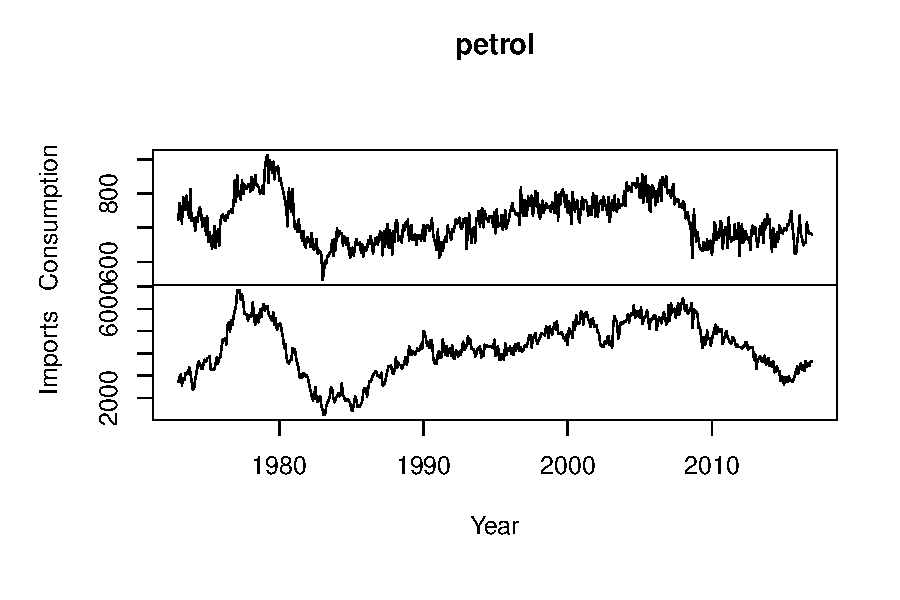
\includegraphics[]{petrol_data.pdf}
\caption{Plot of monthly  Industrial Petroleum Consumption and OPEC Oil Imports, 
  Jan 1973 through December 2016 (seasonally adjusted). }
\label{fig:petroldata}
\end{center}
\end{figure}  

\begin{Example} {\bf Petrol MB Replication.} \rm
\label{exam:petrol-mb}
We now  study the  MB trend filter arising from a LLM  
(cf. Example \ref{exam:trend-i1}) fitted
 to a   bivariate petroleum series:
  Industrial Petroleum Consumption and OPEC Oil Imports, Jan 1973 through December 2016,
 both seasonally adjusted  (displayed in Figure \ref{fig:petroldata}).
   The MLEs for the model parameters are  given by
\[
 \Sigma_{W} = \left[ \begin{array}{ll} 
   2.32 \cdot 10^{-4} &  5.04 \cdot 10^{-4} \\
   5.04 \cdot 10^{-4}  & 34.73 \cdot 10^{-4}  \end{array}  \right]
 \qquad  \Sigma_{Z} = \left[ \begin{array}{ll}
        110.44 \cdot 10^{-5} &  7.17 \cdot 10^{-5}  \\
        7.17 \cdot 10^{-5} & 128.57 \cdot 10^{-5}   \end{array} \right].
\]
  Because the trend variance for the second component is $15$ times 
  larger than that of the first component,
 the corresponding trend filter  does less smoothing. 
 From this fitted model,  we can construct both the WK filter -- recall Exercise
  \ref{exer:trend-i1}, and the plot of the WK filter's frf in Figure \ref{fig:llm-frf} --
  and the optimal concurrent filter via (\ref{eq:wiener-hopf}).
\end{Example}

\begin{Exercise} {\bf Petrol MB Replication.}  \rm
\label{exer:petrol-mb}
 The purpose of this exercise is to demonstrate that MDFA can replicate
 a MB concurrent filter, and even have superior performance when the 
 model is mis-specified. 
 Simulate a sample of size $T=5000$ from an LLM process with parameters
 given in Example \ref{exam:petrol-mb}.   Apply the WK trend filter
(truncate the filter to $1000$ coefficients on each side) and the 
 optimal concurrent trend filter.  
 Use the moving average filter  MDFA  for an $I(1)$ process  to find the best
 concurrent filter, setting $q= 30$.
    Apply both concurrent filters (MB and MDFA)
 to the simulation, and compare the relevant portions to the ideal trend.
 Also determine the in-sample performance, in comparison to the criterion value
 (\ref{eq:opt.val.mdfa-constrained}).   Target the trends for both time series.
\end{Exercise}


\begin{Schunk}
\begin{Sinput}
> # Simulate a Gaussian LLM  of sample size 5000:
> set.seed(1234)
> T.sim <- 5000
> burn <- 1000
> N <- 2
> psi.sim <- c(2.17150287559847, -8.36795922528, -6.04133725367594, 
+              0.0648981656699, -6.80849700177184, -6.66004335288479, 
+              -0.00016098322952, 0.00051984185863)
> psi.sim[7:8] <- c(0,0)
> len <- 1000
> dpoly <- c(1,-1)
> delta <- array(t(dpoly) %x% diag(N),c(N,N,2))
> d <- length(dpoly) - 1
> mu.sim <- mdfa.wnsim(psi.sim[1:3],rep(1,N),T.sim+burn,Inf)
> Sigma.mu <- mu.sim[[2]]
> mu.sim <- mdfa.ucsim(delta,mu.sim[[1]])[(burn+1-d):(T.sim+burn-d),]
> irr.sim <- mdfa.wnsim(psi.sim[4:6],rep(1,N),T.sim,Inf)
> Sigma.irr <- irr.sim[[2]]
> irr.sim <- irr.sim[[1]] 
> x.sim <- mu.sim + irr.sim
> # construct and apply MB WK  and concurrent filters
> grid <- T.sim - d
> iden <- array(diag(N),c(N,N,1))
> f.mu <- mdfa.spectra(iden,iden,Sigma.mu,grid)
> f.irr <- mdfa.spectra(iden,iden,Sigma.irr,grid)
> trend.wkfrf <- mdfa.wkfrf(iden,delta,f.irr,f.mu)
> trend.wkfilter <- mdfa.coeff(trend.wkfrf,-len,len)
> x.trend.ideal <- mvar.filter(x.sim,trend.wkfilter)
> ## HERE :  need to debug mdfa.whfrf
> #trend.whfrf <- mdfa.whfrf(iden,delta,f.irr,f.mu,len)
> #trend.whfilter <- mdfa.coeff(trend.whfrf,-len,len)
>  
> # get MDFA concurrent filter
> q <- 30
> x.diff <- filter(x.sim,dpoly,method="convolution",sides=1)[(d+1):T.sim,]
> spec.hat <- mdfa.pergram(x.diff,dpoly)
> m <- floor(grid/2)
> # The Fourier frequencies
> freq.ft <- 2*pi*grid^{-1}*(seq(1,grid) - (m+1))
> constraints.mdfa <- mdfa.getconstraints(trend.wkfrf,0,NULL,0*diag(N),q)
> bw.mdfa <- mdfa.filter(trend.wkfrf,spec.hat,constraints.mdfa[[1]],constraints.mdfa[[2]])
> x.trend.mdfa <- mvar.filter(x.sim,bw.mdfa[[1]])[(len-q+2):(T-q+1-len),]
> # compare in-sample performance
> print(c(mean((x.trend.ideal[,1] - x.trend.mdfa[,1])^2),
+ 	mean((x.trend.ideal[,2] - x.trend.mdfa[,2])^2)))
\end{Sinput}
\begin{Soutput}
[1] 0.0001415281 0.0001757378
\end{Soutput}
\begin{Sinput}
> # compare to criterion value
> diag(bw.mdfa[[2]])
\end{Sinput}
\begin{Soutput}
[1] 0.0001414576 0.0001794452
\end{Soutput}
\end{Schunk}


\begin{Exercise} {\bf Petrol MB Out-Performance.}  \rm
\label{exer:petrol-mb2}
 Now we alter the specification of the LLM for the Petrol series,
  to illustrate that MDFA can out-perform the MB concurrent filter.  
  We do this by substantially increasing the
 variability in the irregular, producing a noisier simulation -- now the MB concurrent will do too little smoothing.  Consider the same MLE for the trend covariance
  matrix as in Exercise \ref{exam:petrol-mb}, but now set the irregular
 covariance matrix to be
\[
   \qquad  \Sigma_{Z} = \left[ \begin{array}{ll}
       18.32 \cdot 10^{-3}  &  1.19 \cdot 10^{-3}   \\
       1.19 \cdot 10^{-3}  &  18.39 \cdot 10^{-3}  \end{array} \right].
\]
 Simulate a sample of size $T=5000$ from an LLM process with these parameters,
 but apply  the WK trend filter
(truncate the filter to $1000$ coefficients on each side) and the 
 optimal concurrent trend filter  corresponding to the parameters
  given in Example \ref{exam:petrol-mb}.  
 Use the moving average filter  MDFA  for an $I(1)$ process  to find the best
 concurrent filter, setting $q= 30$.
    Apply both concurrent filters (MB and MDFA)
 to the simulation, and compare the relevant portions to the ideal trend.
 Also determine the in-sample performance, in comparison to the criterion value
 (\ref{eq:opt.val.mdfa-constrained}).   Target the trends for both time series.
\end{Exercise}

\begin{Exercise} {\bf Petrol MB Empirical Performance.}  \rm
\label{exer:petrol-mb3}
 We now examine the performance of MDFA   on the Petroleum data itself,
 recognizing that the LLM might be mis-specified.  
 Use the target filter resulting from the MLEs of the fitted LLM,
  from Example \ref{exam:petrol-mb}, truncating five years of observations at either end
   of the series.  
 Apply the  MDFA  for an $I(1)$ process  to find the best
 concurrent filter, setting $q= 30$.
  Apply both concurrent filters (MB and MDFA)
 to the data, and compare the relevant portions to the ideal trend.
 Also determine the in-sample performance, in comparison to the criterion value
 (\ref{eq:opt.val.mdfa-constrained}).   Target the trends for both time series.
\end{Exercise}
    
   
HERE  some discussion, and tables summarizing the results    
   
% \begin{table}[!htb]
% \centering
% \begin{tabular}{cllllll}
% \hline
% & \multicolumn{2}{c}{Null LLM} &\multicolumn{2}{c}{Alternative LLM} & \multicolumn{2}{c}{Petrol Data} \\
% \hline
%   Series 	 &  MB    &  MDFA  &  MB    &  MDFA    &  MB    &  MDFA   \\
%   Consumption &   .1285 & .1268 &  1.3224  &  .9841    &   .1295 &   .1176 \\
%   Imports	 &  .1728 & .1691 &   .8433  &  .6603    &   2.1691  &   2.2033 \\
% \hline
% \end{tabular}
% \caption{\baselineskip=10pt Empirical LPP MSE for real-time trend estimators (MB Concurrent filter versus
%  MDFA filter) applied to bivariate LLM null process,  LLM alternative process,
%  and Petrol data,  with target trend
%  given by the null LLM MB trend. (Units of $10^{-3}$.) }
% \label{tab:petrol.llm.mdfa}
% \end{table}


% \begin{figure}[htb!]
% \centering
% \includegraphics[]{petrolLLMtrendsAlt}
% \caption{\baselineskip=10pt Bivariate  trend  filter applied to alternative LLM simulation (grey), with trends in black. 
%  The simulation is obtained from altering the paramteres of an 
%  LLM fitted to bivariate Petrol (Consumption and Imports), so the component
%  series of the simulation are labelled accordingly.}
% \label{fig:llm.alttrends}
% \end{figure}



% 
% \begin{figure}[htb!]
% \centering
% \includegraphics[]{petrolLLMrealtimeData}
% \caption{\baselineskip=10pt  Monthly Petroleum data:  LLM bivariate  trend  output (black), 
% with non-stationary MDFA trend (dark grey) and MB concurrent trend (light grey). 
% The trend lines have been vertically staggered for easier visualization.}
% \label{fig:llm.datamdfa}
% \end{figure}

 




HERE  STM replicate, MDFA for mis-spec, and Ndc.  Connect to HP
 

HERE  Seasonal UC replicate, MDFA for mis-sec, and Starts


% Exercise 1
% 
% # Simulate a Gaussian VAR(1)  
% T.sim <- 500 + 2*len
% N <- 2
% phi.matrix <- rbind(c(1,.5),c(-.2,.3))
% innovar.matrix <- diag(N)
% true.psidelta <- var1.par2psi(phi.matrix,100)
% gamma.0 <- matrix(solve(diag(N^2) - phi.matrix %x% phi.matrix) %*% 
% 	matrix(innovar.matrix,ncol=1),nrow=N)
% x.init <- t(chol(gamma.0)) %*% rnorm(N)
% x.next <- x.init
% x.sim <- NULL
% for(t in 1:T.sim)
% {
% 	x.next <- phi.matrix %*% x.next + rnorm(N)
% 	x.sim <- cbind(x.sim,x.next)
% }
% x.sim <- ts(t(x.sim))
% x.acf <- acf(x.sim,type="covariance",plot=FALSE,lag.max=T.sim)[[1]]
% x.acf <- aperm(aperm(x.acf,c(3,2,1)),c(2,1,3))
% 
% # construct and apply BW filter
% bw.filter <- wk.trend[[1]]
% x.trend.bw11 <- filter(x.sim[,1],bw.filter[1,1,],method="convolution",sides=2)
% x.trend.bw12 <- filter(x.sim[,2],bw.filter[1,2,],method="convolution",sides=2)
% x.trend.bw21 <- filter(x.sim[,1],bw.filter[2,1,],method="convolution",sides=2)
% x.trend.bw22 <- filter(x.sim[,2],bw.filter[2,2,],method="convolution",sides=2)
% x.trend.bw <- cbind(x.trend.bw11 + x.trend.bw12,x.trend.bw21 + x.trend.bw22)
% x.trend.bw <- x.trend.bw[(len+1):(T.sim-len),] 
%  
% 
% # visualize
% pdf(file="petrolVAR1trends.pdf",width=4, height=4.6)
% par(oma=c(2,0,0,0),mar=c(2,4,2,2)+0.1,mfrow=c(2,1),cex.lab=.8)
% plot(ts(x.sim[(len+1):(T.sim-len),1]),ylab="Series 1",xlab="",yaxt="n",xaxt="n",col=grey(.7))
% axis(1,cex.axis=.5)
% axis(2,cex.axis=.5)
% lines(x.trend.bw[,1],col=1,lwd=2)
% #lines(ts(x.sim[(len+1):(T.sim-len),1]))
% plot(ts(x.sim[(len+1):(T.sim-len),2]),ylab="Series 2",xlab="",yaxt="n",xaxt="n",col=grey(.7))
% axis(1,cex.axis=.5)
% axis(2,cex.axis=.5)
% lines(x.trend.bw[,2],col=1,lwd=2)
% #lines(ts(x.sim[(len+1):(T.sim-len),2]))
% mtext("Time", side = 1, line = 1,outer=TRUE)
% dev.off()
% 
% # get LPP soln using true VAR(1)
% A.next <- diag(2)
% A.phi <- matrix(0,2,2)
% for(j in 1:len)
% {
% 	A.next <- A.next %*% phi.matrix
% 	A.phi <- A.phi + bw.filter[,,(len+1-j)] %*% A.next
% }
% bw.lpp <- bw.filter[,,(len+1):(2*len+1)]
% bw.lpp[,,1] <- bw.lpp[,,1] + A.phi
% 
% 
% # get MDFA concurrent filter
% q <- 30
% Grid <- T.sim
% frf.trend <- mdfa.frf(wk.trend[[1]],len,Grid)
% spec.hat <- mdfa.pergram(x.sim,1)
% # choose one of the four constraint scenarios for MDFA	
% bw.mdfa <- mdfa.unconstrained(frf.trend,spec.hat,q)
% bw.mdfa <- mdfa.levelconstraint(frf.trend,spec.hat,q)
% bw.mdfa <- mdfa.tsconstraint(frf.trend,spec.hat,q)
% bw.mdfa <- mdfa.ltsconstraint(frf.trend,spec.hat,q)
%  
% # apply the MDFA concurrent filter
% x.trend.mdfa11 <- filter(x.sim[,1],bw.mdfa[[1]][1,1,],method="convolution",sides=1)
% x.trend.mdfa12 <- filter(x.sim[,2],bw.mdfa[[1]][1,2,],method="convolution",sides=1)
% x.trend.mdfa21 <- filter(x.sim[,1],bw.mdfa[[1]][2,1,],method="convolution",sides=1)
% x.trend.mdfa22 <- filter(x.sim[,2],bw.mdfa[[1]][2,2,],method="convolution",sides=1)
% x.trend.mdfa <- cbind(x.trend.mdfa11 + x.trend.mdfa12,x.trend.mdfa21 + x.trend.mdfa22)
% x.trend.mdfa <- x.trend.mdfa[(len+1):(T.sim-len),] 
% 
% # construct and apply concurrent BW filter
% conc.filter <- conc.trend
% x.trend.conc11 <- filter(x.sim[,1],rev(conc.filter[1,1,]),method="convolution",sides=1)
% x.trend.conc12 <- filter(x.sim[,2],rev(conc.filter[1,2,]),method="convolution",sides=1)
% x.trend.conc21 <- filter(x.sim[,1],rev(conc.filter[2,1,]),method="convolution",sides=1)
% x.trend.conc22 <- filter(x.sim[,2],rev(conc.filter[2,2,]),method="convolution",sides=1)
% x.trend.conc <- cbind(x.trend.conc11 + x.trend.conc12,x.trend.conc21 + x.trend.conc22)
% x.trend.conc <- x.trend.conc[(len+1):(T.sim-len),] 
% 
% # construct and apply optimal LPP filter
% x.trend.lpp11 <- filter(x.sim[,1],bw.lpp[1,1,],method="convolution",sides=1)
% x.trend.lpp12 <- filter(x.sim[,2],bw.lpp[1,2,],method="convolution",sides=1)
% x.trend.lpp21 <- filter(x.sim[,1],bw.lpp[2,1,],method="convolution",sides=1)
% x.trend.lpp22 <- filter(x.sim[,2],bw.lpp[2,2,],method="convolution",sides=1)
% x.trend.lpp <- cbind(x.trend.lpp11 + x.trend.lpp12,x.trend.lpp21 + x.trend.lpp22)
% x.trend.lpp <- x.trend.lpp[(len+1):(T.sim-len),] 
% 
% 
% 
% # visualize
% par(oma=c(2,0,0,0),mar=c(2,4,2,2)+0.1,mfrow=c(2,1),cex.lab=.8)
% plot(ts(x.trend.bw[,1]),ylab="",xlab="",yaxt="n",xaxt="n",col=1,lwd=1,
% 	ylim=c(min(x.trend.bw[,1])-4,max(x.trend.bw[,1])))
% axis(1,cex.axis=.5)
% axis(2,cex.axis=.5)
% lines(x.trend.mdfa[,1]-2,col=grey(.4),lwd=1,lty=1)
% lines(x.trend.lpp[,1]-4,col=grey(.6),lwd=1,lty=1)
% plot(ts(x.trend.bw[,2]),ylab="",xlab="",yaxt="n",xaxt="n",col=1,lwd=1,
% 	ylim=c(min(x.trend.bw[,2])-4,max(x.trend.bw[,2])))
% axis(1,cex.axis=.5)
% axis(2,cex.axis=.5)
% lines(x.trend.mdfa[,2]-2,col=grey(.4),lwd=1,lty=1)
% lines(x.trend.lpp[,2]-4,col=grey(.6),lwd=1,lty=1)
% mtext("Time", side = 1, line = 1,outer=TRUE)
%  
% # compare in-sample performance: MDFA for series, and then Conc for series
% print(c(mean((x.trend.bw[,1] - x.trend.mdfa[,1])^2),
% 	mean((x.trend.bw[,2] - x.trend.mdfa[,2])^2)))
% print(c(mean((x.trend.bw[,1] - x.trend.conc[,1])^2),
% 	mean((x.trend.bw[,2] - x.trend.conc[,2])^2)))
% print(c(mean((x.trend.bw[,1] - x.trend.lpp[,1])^2),
% 	mean((x.trend.bw[,2] - x.trend.lpp[,2])^2)))
% 
% # compare to criterion value
% print(diag(bw.mdfa[[2]]))
% 
% 

 

% # construct and apply BW filter
% bw.filter <- wk.trend[[1]]
% x.trend.bw11 <- filter(x.sim[,1],bw.filter[1,1,],method="convolution",sides=2)
% x.trend.bw12 <- filter(x.sim[,2],bw.filter[1,2,],method="convolution",sides=2)
% x.trend.bw21 <- filter(x.sim[,1],bw.filter[2,1,],method="convolution",sides=2)
% x.trend.bw22 <- filter(x.sim[,2],bw.filter[2,2,],method="convolution",sides=2)
% x.trend.bw <- cbind(x.trend.bw11 + x.trend.bw12,x.trend.bw21 + x.trend.bw22)
% x.trend.bw <- x.trend.bw[(len+1):(T.sim-len),] 
% 
% # visualize
% pdf(file="petrolLLMtrendsNull.pdf",width=4, height=4.6)
% par(oma=c(2,0,0,0),mar=c(2,4,2,2)+0.1,mfrow=c(2,1),cex.lab=.8)
% plot(ts(x.sim[(len+1):(T.sim-len),1]),ylab="Consumption",xlab="",yaxt="n",xaxt="n",col=grey(.7))
% axis(1,cex.axis=.5)
% axis(2,cex.axis=.5)
% lines(x.trend.bw[,1],col=1,lwd=1)
% plot(ts(x.sim[(len+1):(T.sim-len),2]),ylab="Imports",xlab="",yaxt="n",xaxt="n",col=grey(.7))
% axis(1,cex.axis=.5)
% axis(2,cex.axis=.5)
% lines(x.trend.bw[,2],col=1,lwd=1)
% mtext("Time", side = 1, line = 1,outer=TRUE)
% dev.off()
% 
% # get MDFA concurrent filter for I(1) case
% q <- 30
% x.diff <- diff(x.sim)
% spec.hat <- mdfa.pergram(x.diff,c(1,-1))
% Grid <- T.sim - 1
% frf.trend <- mdfa.frf(wk.trend[[1]],len,Grid)
% #bw.mdfa <- mdfa.levelconstraint(frf.trend,spec.hat,q)[[1]]
% constraints.mdfa <- mdfa.getconstraints(frf.trend,0,NULL,q)
% bw.mdfa <- mdfa.filter(frf.trend,spec.hat,constraints.mdfa[[1]],constraints.mdfa[[2]])[[1]]
% 
% # apply the MDFA concurrent filter
% x.trend.mdfa11 <- filter(x.sim[,1],bw.mdfa[1,1,],method="convolution",sides=1)
% x.trend.mdfa12 <- filter(x.sim[,2],bw.mdfa[1,2,],method="convolution",sides=1)
% x.trend.mdfa21 <- filter(x.sim[,1],bw.mdfa[2,1,],method="convolution",sides=1)
% x.trend.mdfa22 <- filter(x.sim[,2],bw.mdfa[2,2,],method="convolution",sides=1)
% x.trend.mdfa <- cbind(x.trend.mdfa11 + x.trend.mdfa12,x.trend.mdfa21 + x.trend.mdfa22)
% x.trend.mdfa <- x.trend.mdfa[(len+1):(T.sim-len),] 
% 
% # construct and apply concurrent BW filter
% conc.filter <- conc.trend
% x.trend.conc11 <- filter(x.sim[,1],rev(conc.filter[1,1,]),method="convolution",sides=1)
% x.trend.conc12 <- filter(x.sim[,2],rev(conc.filter[1,2,]),method="convolution",sides=1)
% x.trend.conc21 <- filter(x.sim[,1],rev(conc.filter[2,1,]),method="convolution",sides=1)
% x.trend.conc22 <- filter(x.sim[,2],rev(conc.filter[2,2,]),method="convolution",sides=1)
% x.trend.conc <- cbind(x.trend.conc11 + x.trend.conc12,x.trend.conc21 + x.trend.conc22)
% x.trend.conc <- x.trend.conc[(len+1):(T.sim-len),] 
% 
% # visualize
% pdf(file="petrolLLMrealtimeNull.pdf",width=4, height=4.6)
% par(oma=c(2,0,0,0),mar=c(2,4,2,2)+0.1,mfrow=c(2,1),cex.lab=.8)
% plot(ts(x.trend.bw[,1]),ylab="Consumption",xlab="",yaxt="n",xaxt="n",col=1,lwd=1,
% 	ylim=c(min(x.trend.bw[,1])-2/2,max(x.trend.bw[,1])))
% axis(1,cex.axis=.5)
% axis(2,cex.axis=.5)
% lines(x.trend.mdfa[,1]-1/2,col=grey(.4),lwd=1,lty=1)
% lines(x.trend.conc[,1]-2/2,col=grey(.6),lwd=1,lty=1)
% plot(ts(x.trend.bw[,2]),ylab="Imports",xlab="",yaxt="n",xaxt="n",col=1,lwd=1,
% 	ylim=c(min(x.trend.bw[,2])-2,max(x.trend.bw[,2])))
% axis(1,cex.axis=.5)
% axis(2,cex.axis=.5)
% lines(x.trend.mdfa[,2]-1,col=grey(.4),lwd=1,lty=1)
% lines(x.trend.conc[,2]-2,col=grey(.6),lwd=1,lty=1)
% mtext("Time", side = 1, line = 1,outer=TRUE)
% dev.off()
%  
% # compare in-sample performance: MDFA for series, and then Conc for series
% print(c(mean((x.trend.bw[,1] - x.trend.mdfa[,1])^2),
% 	mean((x.trend.bw[,2] - x.trend.mdfa[,2])^2)))
% print(c(mean((x.trend.bw[,1] - x.trend.conc[,1])^2),
% 	mean((x.trend.bw[,2] - x.trend.conc[,2])^2)))
% 
% 



%  note: MDFA_con replaces Constraints,
%    includes material from Replication

%------------------------------------------------------------------

% Chapter 5
%\SweaveInput{Integrated}
%  note: includes material from Cointegrated

%----------------------------------------

% Chapter 6
%\SweaveInput{Custom}
%  note: Custom replaces ATS and ATS_multivariate

%------------------------------------------

% Chapter 7
%  regularization, shrinkage towards null specification
%\SweaveInput{Regularization}

%-------------------------------------------------------------

%  Chapter 8
%\SweaveInput{Filter_revisions}
%\SweaveInput{Vintage}
%  note: Vintage replaces Filter_revisions

%----------------------------------------------

%  Chapter 9
% embedding in SVF,  backcasting GDP
%\SweaveInput{Mixed}

%--------------------------------------------------------------------

%\SweaveInput{Summary}

%--------------------------------------------------------------------

\begin{thebibliography}{99}

\bibitem{} Ansley, C. F. and R. Kohn (1986).
A note on reparameterizing a vector autoregressive moving average
model to enforce stationarity. 
  Journal of Statistical Computation and Simulation 24, 99-106.
  
\bibitem{}  Ansley, C. F. and P. Newbold (1979). Multivariate partial autocorrelations. 
  In Proceedings of the Businessand Economics Section, pp. 349-353.
  American Statistical Association.

\bibitem{} Baxter, M., and King, R. G. (1999). Measuring business cycles: approximate band-pass filters for economic time series. Review of economics and statistics, 81(4), 575-593.

\bibitem{} Bell, W. (1984). Signal extraction for nonstationary time series. The Annals of Statistics, 12(2), 646-664.

\bibitem{}  Bell, W. and Martin, D. (2004) Computation of asymmetric signal 
 extraction filters and mean  squared error for ARIMA component models.  
 {\it Journal of Time Series Analysis} {\bf 25}, 603--625.

\bibitem{} Brockwell, P.J., and Davis, R.A. (1991).  
  Time Series: Theory and Methods, second edition.   Springer. New York.

\bibitem{} Christiano, L.J., and Fitzgerald, T.J.(2003). 
  The band pass filter.  International economic review 44 (2), 435-465.

\bibitem{} Golub, G. H., and Van Loan, C. F. (1996). Matrix Computations Johns Hopkins University Press. Baltimore and London.


\bibitem{} Heaps, S.E., 2020. Enforcing stationarity through the prior in vector autoregressions. arXiv preprint arXiv:2004.09455.

\bibitem{} Hosoya, Y., and Taniguchi, M. (1982). A central limit theorem for stationary processes and the parameter estimation of linear processes. The Annals of Statistics, 132-153.

\bibitem{} L\"utkepohl, H. (2007).  New Introduction to Multiple Time Series Analysis. 
Springer-Verlag. 

\bibitem{} McElroy, T. (2008a). Matrix formulas for nonstationary ARIMA signal extraction. Econometric Theory, 988-1009.

\bibitem{} McElroy, T. (2008b). Exact formulas for the Hodrick-Prescott filter.
  The Econometrics Journal, 11(1), pp.209-217.

\bibitem{} McElroy, T. (2018). Recursive Computation for Block-Nested Covariance Matrices. Journal of Time Series Analysis, 39(3), pp.299-312.

\bibitem{} McElroy, T. and Findley, D. (2010). 
   Discerning Between Models Through Multi-Step Ahead
Forecasting Errors. Journal of Statistical Planning and Inference 140, 3655-3675.

\bibitem{} McElroy, T., and Findley, D. (2015). Fitting constrained vector autoregression models. In Empirical Economic and Financial Research (pp. 451-470). Springer, Cham.

\bibitem{} McElroy, T., and Trimbur, T. (2015). Signal Extraction for Non-Stationary Multivariate Time Series with Illustrations for Trend Inflation. Journal of Time 
Series Analysis, 36(2), 209-227.


\bibitem{} McElroy, T. S. and Wildi, M. (2020). The multivariate linear prediction problem: model-based and direct filtering solutions. Econometrics and Statistics, 14, 112-130.

\bibitem{} Self, S. G., and Liang, K. Y. (1987). Asymptotic properties of maximum likelihood estimators and likelihood ratio tests under nonstandard conditions. Journal of the American Statistical Association, 82(398), 605-610.

\bibitem{} Taniguchi, M., and Kakizawa, Y. (2012). Asymptotic theory of statistical inference for time series. Springer Science \& Business Media.

\bibitem{} Wildi, M. (2007). Real-Time Signal Extraction.

\bibitem{} Wildi, M. and McElroy, T. (2016). Optimal real-time filters for linear prediction problems. Journal of Time Series Econometrics, 8(2), pp.155-192.

\end{thebibliography}


\end{document}


OLD IDEAS

%-------------------------------------------

%\SweaveInput{Exotic_pub}

%----------------------------------------------

%\SweaveInput{Inference}

%------------------------------------------------------------------
 
%\SweaveInput{Adaptive}

%--------------------------------------------------------------------

%\SweaveInput{Seasonal_adjustment}
%--------------------------------------------------------------------

%\SweaveInput{Appendix}


